% Options for packages loaded elsewhere
% Options for packages loaded elsewhere
\PassOptionsToPackage{unicode}{hyperref}
\PassOptionsToPackage{hyphens}{url}
\PassOptionsToPackage{dvipsnames,svgnames,x11names}{xcolor}
%
\documentclass[
  a4paper,
  DIV=11,
  numbers=noendperiod]{scrartcl}
\usepackage{xcolor}
\usepackage[margin=2.2cm]{geometry}
\usepackage{amsmath,amssymb}
\setcounter{secnumdepth}{5}
\usepackage{iftex}
\ifPDFTeX
  \usepackage[T1]{fontenc}
  \usepackage[utf8]{inputenc}
  \usepackage{textcomp} % provide euro and other symbols
\else % if luatex or xetex
  \usepackage{unicode-math} % this also loads fontspec
  \defaultfontfeatures{Scale=MatchLowercase}
  \defaultfontfeatures[\rmfamily]{Ligatures=TeX,Scale=1}
\fi
\usepackage{lmodern}
\ifPDFTeX\else
  % xetex/luatex font selection
\fi
% Use upquote if available, for straight quotes in verbatim environments
\IfFileExists{upquote.sty}{\usepackage{upquote}}{}
\IfFileExists{microtype.sty}{% use microtype if available
  \usepackage[]{microtype}
  \UseMicrotypeSet[protrusion]{basicmath} % disable protrusion for tt fonts
}{}
\makeatletter
\@ifundefined{KOMAClassName}{% if non-KOMA class
  \IfFileExists{parskip.sty}{%
    \usepackage{parskip}
  }{% else
    \setlength{\parindent}{0pt}
    \setlength{\parskip}{6pt plus 2pt minus 1pt}}
}{% if KOMA class
  \KOMAoptions{parskip=half}}
\makeatother
% Make \paragraph and \subparagraph free-standing
\makeatletter
\ifx\paragraph\undefined\else
  \let\oldparagraph\paragraph
  \renewcommand{\paragraph}{
    \@ifstar
      \xxxParagraphStar
      \xxxParagraphNoStar
  }
  \newcommand{\xxxParagraphStar}[1]{\oldparagraph*{#1}\mbox{}}
  \newcommand{\xxxParagraphNoStar}[1]{\oldparagraph{#1}\mbox{}}
\fi
\ifx\subparagraph\undefined\else
  \let\oldsubparagraph\subparagraph
  \renewcommand{\subparagraph}{
    \@ifstar
      \xxxSubParagraphStar
      \xxxSubParagraphNoStar
  }
  \newcommand{\xxxSubParagraphStar}[1]{\oldsubparagraph*{#1}\mbox{}}
  \newcommand{\xxxSubParagraphNoStar}[1]{\oldsubparagraph{#1}\mbox{}}
\fi
\makeatother


\usepackage{longtable,booktabs,array}
\newcounter{none} % for unnumbered tables
\usepackage{calc} % for calculating minipage widths
% Correct order of tables after \paragraph or \subparagraph
\usepackage{etoolbox}
\makeatletter
\patchcmd\longtable{\par}{\if@noskipsec\mbox{}\fi\par}{}{}
\makeatother
% Allow footnotes in longtable head/foot
\IfFileExists{footnotehyper.sty}{\usepackage{footnotehyper}}{\usepackage{footnote}}
\makesavenoteenv{longtable}
\usepackage{graphicx}
\makeatletter
\newsavebox\pandoc@box
\newcommand*\pandocbounded[1]{% scales image to fit in text height/width
  \sbox\pandoc@box{#1}%
  \Gscale@div\@tempa{\textheight}{\dimexpr\ht\pandoc@box+\dp\pandoc@box\relax}%
  \Gscale@div\@tempb{\linewidth}{\wd\pandoc@box}%
  \ifdim\@tempb\p@<\@tempa\p@\let\@tempa\@tempb\fi% select the smaller of both
  \ifdim\@tempa\p@<\p@\scalebox{\@tempa}{\usebox\pandoc@box}%
  \else\usebox{\pandoc@box}%
  \fi%
}
% Set default figure placement to htbp
\def\fps@figure{htbp}
\makeatother





\setlength{\emergencystretch}{3em} % prevent overfull lines

\providecommand{\tightlist}{%
  \setlength{\itemsep}{0pt}\setlength{\parskip}{0pt}}



 


\usepackage{fvextra}
\DefineVerbatimEnvironment{Highlighting}{Verbatim}{breaklines,commandchars=\\\{\}}
\KOMAoption{captions}{tableheading}
\makeatletter
\@ifpackageloaded{caption}{}{\usepackage{caption}}
\AtBeginDocument{%
\ifdefined\contentsname
  \renewcommand*\contentsname{Table of contents}
\else
  \newcommand\contentsname{Table of contents}
\fi
\ifdefined\listfigurename
  \renewcommand*\listfigurename{List of Figures}
\else
  \newcommand\listfigurename{List of Figures}
\fi
\ifdefined\listtablename
  \renewcommand*\listtablename{List of Tables}
\else
  \newcommand\listtablename{List of Tables}
\fi
\ifdefined\figurename
  \renewcommand*\figurename{Figure}
\else
  \newcommand\figurename{Figure}
\fi
\ifdefined\tablename
  \renewcommand*\tablename{Table}
\else
  \newcommand\tablename{Table}
\fi
}
\@ifpackageloaded{float}{}{\usepackage{float}}
\floatstyle{ruled}
\@ifundefined{c@chapter}{\newfloat{codelisting}{h}{lop}}{\newfloat{codelisting}{h}{lop}[chapter]}
\floatname{codelisting}{Listing}
\newcommand*\listoflistings{\listof{codelisting}{List of Listings}}
\makeatother
\makeatletter
\makeatother
\makeatletter
\@ifpackageloaded{caption}{}{\usepackage{caption}}
\@ifpackageloaded{subcaption}{}{\usepackage{subcaption}}
\makeatother
\usepackage{bookmark}
\IfFileExists{xurl.sty}{\usepackage{xurl}}{} % add URL line breaks if available
\urlstyle{same}
% fallback for those not using the hyperref driver hyperxmp:
\makeatletter
\@ifundefined{xmpquote}{\newcommand{\xmpquote}[1]{#1}}{}
\makeatother
\hypersetup{
  pdftitle={Stock coordination of turbot in the North Sea (tur.27.4)},
  pdfauthor={Lennert van de Pol (Wageningen Marine Research)},
  colorlinks=true,
  linkcolor={blue},
  filecolor={Maroon},
  citecolor={Blue},
  urlcolor={Blue},
  pdfcreator={LaTeX via pandoc}}


\title{Stock coordination of turbot in the North Sea (tur.27.4)}
\usepackage{etoolbox}
\makeatletter
\providecommand{\subtitle}[1]{% add subtitle to \maketitle
  \apptocmd{\@title}{\par {\large #1 \par}}{}{}
}
\makeatother
\subtitle{From the converted InterCatch data to the Catch Combined and
the Distributions Combined, catch year 2025 (WGNSSK 2026)}
\author{Lennert van de Pol (Wageningen Marine Research)}
\date{21 October 2026}
\begin{document}
\maketitle

\renewcommand*\contentsname{Table of contents}
{
\setcounter{tocdepth}{3}
\tableofcontents
}

\section{The stock coordination in
short}\label{the-stock-coordination-in-short}

The stock coordination is the step between the national data and the
stock assessment. Every country reports what its fleets caught of the
stock, by \emph{stratum} - a combination of country, catch category
(landings or discards), season, area and fleet - and what was measured
of it: the age distribution of the fish that were sampled. Two things
are missing from that picture. Discards are observed by sampling
programmes, so not every stratum that lands brill has a discard
estimate. And age samples are taken in a part of the strata only. The
stock coordinator fills in both and adds everything up into the two
tables that the stock coordination format (SCF v4) asks for:

\begin{itemize}
\tightlist
\item
  \textbf{Catch Combined (CC)}: the catch of the stock in tonnes, by
  year and catch category;
\item
  \textbf{Distributions Combined (DC)}: the numbers (in thousands of
  fish) and the mean weight (in g) at age of that catch, by catch
  category.
\end{itemize}

This report follows the data of brill in Subarea 4 and divisions 3.a and
7.d-e (\emph{Scophthalmus rhombus}, \texttt{bll.27.3a47de}) from the
InterCatch files of the working group for the catch year 2025 to those
two tables, in the steps below. Everything is done in R with the package
\texttt{rcef}: the raising and the allocation use the functions of the
RDBESStockCoord framework (\texttt{catchRaising()} and
\texttt{catchAllocationAoL()}), the two final tables are made by
\texttt{catchCombined()} and \texttt{distributionsCombined()}, and the
figures come from the exploration functions of the package.

The steps are the scripts of the TAF project, run in this order; each
leaves the files the next one reads:

\begin{enumerate}
\def\labelenumi{\arabic{enumi}.}
\tightlist
\item
  \textbf{Data} (\texttt{data.R}): the InterCatch data are converted to
  the CEF format and the columns the groups are written on are derived.
  Files: \texttt{data/catch\_data\_CEF.csv} and
  \texttt{data/distributions\_data\_CEF.csv}.
\item
  \textbf{Discard raising} (\texttt{model\_discard\_raising.R}): the
  landings without a discard estimate get one, from the discard ratio of
  a group of comparable strata. File:
  \texttt{model/catch\_data\_raised.csv}.
\item
  \textbf{age allocation} (\texttt{model\_age\_allocation.R}): every
  stratum without a age distribution gets one, from the distributions of
  a group of comparable strata. Files:
  \texttt{model/catch\_data\_allocated.csv} and
  \texttt{model/distributions\_data\_allocated.csv}.
\item
  \textbf{Aggregation} (\texttt{output.R}): the raised catch and the
  allocated distributions are added up into the CC and the DC. Files:
  \texttt{output/SCF\_CC.csv} and \texttt{output/SCF\_DC.csv}.
\item
  \textbf{Report} (\texttt{report.R} and \texttt{report.qmd}): this
  document, made from the files above and the figures the scripts saved.
  Files: \texttt{report/report.html} and \texttt{report/report.pdf}.
\end{enumerate}

A few words are used throughout:

\begin{itemize}
\tightlist
\item
  a \textbf{stratum} is a row of the catch table: country, catch
  category, season, area and fleet;
\item
  a catch row is \textbf{imported} when it is in the data as it came and
  \textbf{raised} when the raising added it;
\item
  a age distribution is \textbf{sampled} when fish were measured and
  \textbf{estimated} when the allocation made it;
\item
  a \textbf{group} is a set of strata that are raised, or allocated,
  together; its \textbf{donors} (the \emph{matched data}) are the strata
  its ratio, or its distribution, is taken from;
\item
  a \textbf{domain} is a set of strata that share an estimate:
  \texttt{domainCatchDis} ties a landings row to its discard estimate
  and \texttt{domainBiology} ties a stratum to its age distribution.
\end{itemize}

\textbf{In numbers.} The catch of the stock for 2025 is 1,777.3 t:
1,669.5 t of landings and 107.8 t of discards, of which 84.4 t were
reported and 23.4 t raised. The allocation gave a age distribution to
all 298 catch rows: 46 sampled ones (0 fish measured) and 252 estimated
ones; by weight, 39\% of the landings and 9\% of the discards have a
sampled distribution. The DC holds the numbers and the mean weights of
18 age classes of landings and 4 of discards.

\section{The data: the converted InterCatch
data}\label{the-data-the-converted-intercatch-data}

\subsection{From InterCatch to the CEF
format}\label{from-intercatch-to-the-cef-format}

The data are the InterCatch data of the working group for 2025: the
overview files that InterCatch writes for the stock (the stock overview,
the catch and sample data tables and the numbers at age).
\texttt{funICoutCEF()} converts them to the Common Exchange Format (CEF
v17.1), the long format of the national estimates of the RDBES:

\begin{itemize}
\tightlist
\item
  the \textbf{catch table}, a row for each stratum, catch category,
  origin and variable, with the weight of the catch (\texttt{total}) and
  the domains that tie it to its discard estimate and to its age
  distribution;
\item
  the \textbf{distribution table}, a \texttt{Number} row and a
  \texttt{WeightLive} row (the mean weight) for each age class of each
  sampled distribution, with the number of fish measured;
\item
  an effort table, which is not used here.
\end{itemize}

\texttt{derive\_fields()} then adds the columns the groups are written
on: the metier levels (\texttt{metier4}, the gear, down to
\texttt{metier6}), \texttt{mesh}, the ICES area levels and a
\texttt{Stratum} key. It is run once, in \texttt{data.R}, and everything
after it reads those columns.

\subsection{What the data hold}\label{what-the-data-hold}

The converted catch table has 374 records of 10 countries, in 4 areas
and 34 fleets. The working group's own estimate
(\texttt{originType\ =\ WGEstimate}) is what is raised and added up:
1,669.5 t of landings and 84.4 t of discards that were reported. The 24
rows of origin \texttt{Official} weigh 0.0 t and the 24 rows of landings
below the minimum size (BMS) 0.0 t, so neither matters here. The
distribution table has 0 age distributions with 0 fish measured; it has
no age distributions. Table~\ref{tbl-country} shows where they come
from.

\begin{longtable}[]{@{}
  >{\raggedright\arraybackslash}p{(\linewidth - 8\tabcolsep) * \real{0.2658}}
  >{\raggedleft\arraybackslash}p{(\linewidth - 8\tabcolsep) * \real{0.1646}}
  >{\raggedleft\arraybackslash}p{(\linewidth - 8\tabcolsep) * \real{0.1646}}
  >{\raggedleft\arraybackslash}p{(\linewidth - 8\tabcolsep) * \real{0.2278}}
  >{\raggedleft\arraybackslash}p{(\linewidth - 8\tabcolsep) * \real{0.1772}}@{}}

\caption{\label{tbl-country}The converted data by country: the landings
and the discards that were reported (WGEstimate, tonnes), the age
distributions and the fish measured in them.}

\tabularnewline

\toprule\noalign{}
\begin{minipage}[b]{\linewidth}\raggedright
Country
\end{minipage} & \begin{minipage}[b]{\linewidth}\raggedleft
Landings (t)
\end{minipage} & \begin{minipage}[b]{\linewidth}\raggedleft
Discards (t)
\end{minipage} & \begin{minipage}[b]{\linewidth}\raggedleft
age distributions
\end{minipage} & \begin{minipage}[b]{\linewidth}\raggedleft
Fish measured
\end{minipage} \\
\midrule\noalign{}
\endhead
\bottomrule\noalign{}
\endlastfoot
Netherlands & 810.2 & 73.6 & 0 & 0 \\
Denmark & 235.3 & 0.1 & 0 & 0 \\
Germany & 210.0 & 2.7 & 0 & 0 \\
Belgium & 152.8 & 7.5 & 0 & 0 \\
UK (England) & 130.8 & 0.0 & 0 & 0 \\
UK(Scotland) & 107.0 & 0.5 & 0 & 0 \\
Norway & 21.9 & 0.0 & 0 & 0 \\
Sweden & 1.4 & 0.0 & 0 & 0 \\
France & 0.1 & 0.0 & 0 & 0 \\
UK(Northern Ireland) & 0.0 & 0.0 & 0 & 0 \\
Total & 1,669.5 & 84.4 & 0 & 0 \\

\end{longtable}

The beam trawls (TBB) and the otter trawls (OTB) land most of the brill,
and with the trammel nets (GTR) they also have most of the discards that
were reported (Figure~\ref{fig-catch-metier}).

\begin{figure}[htbp]

\centering{

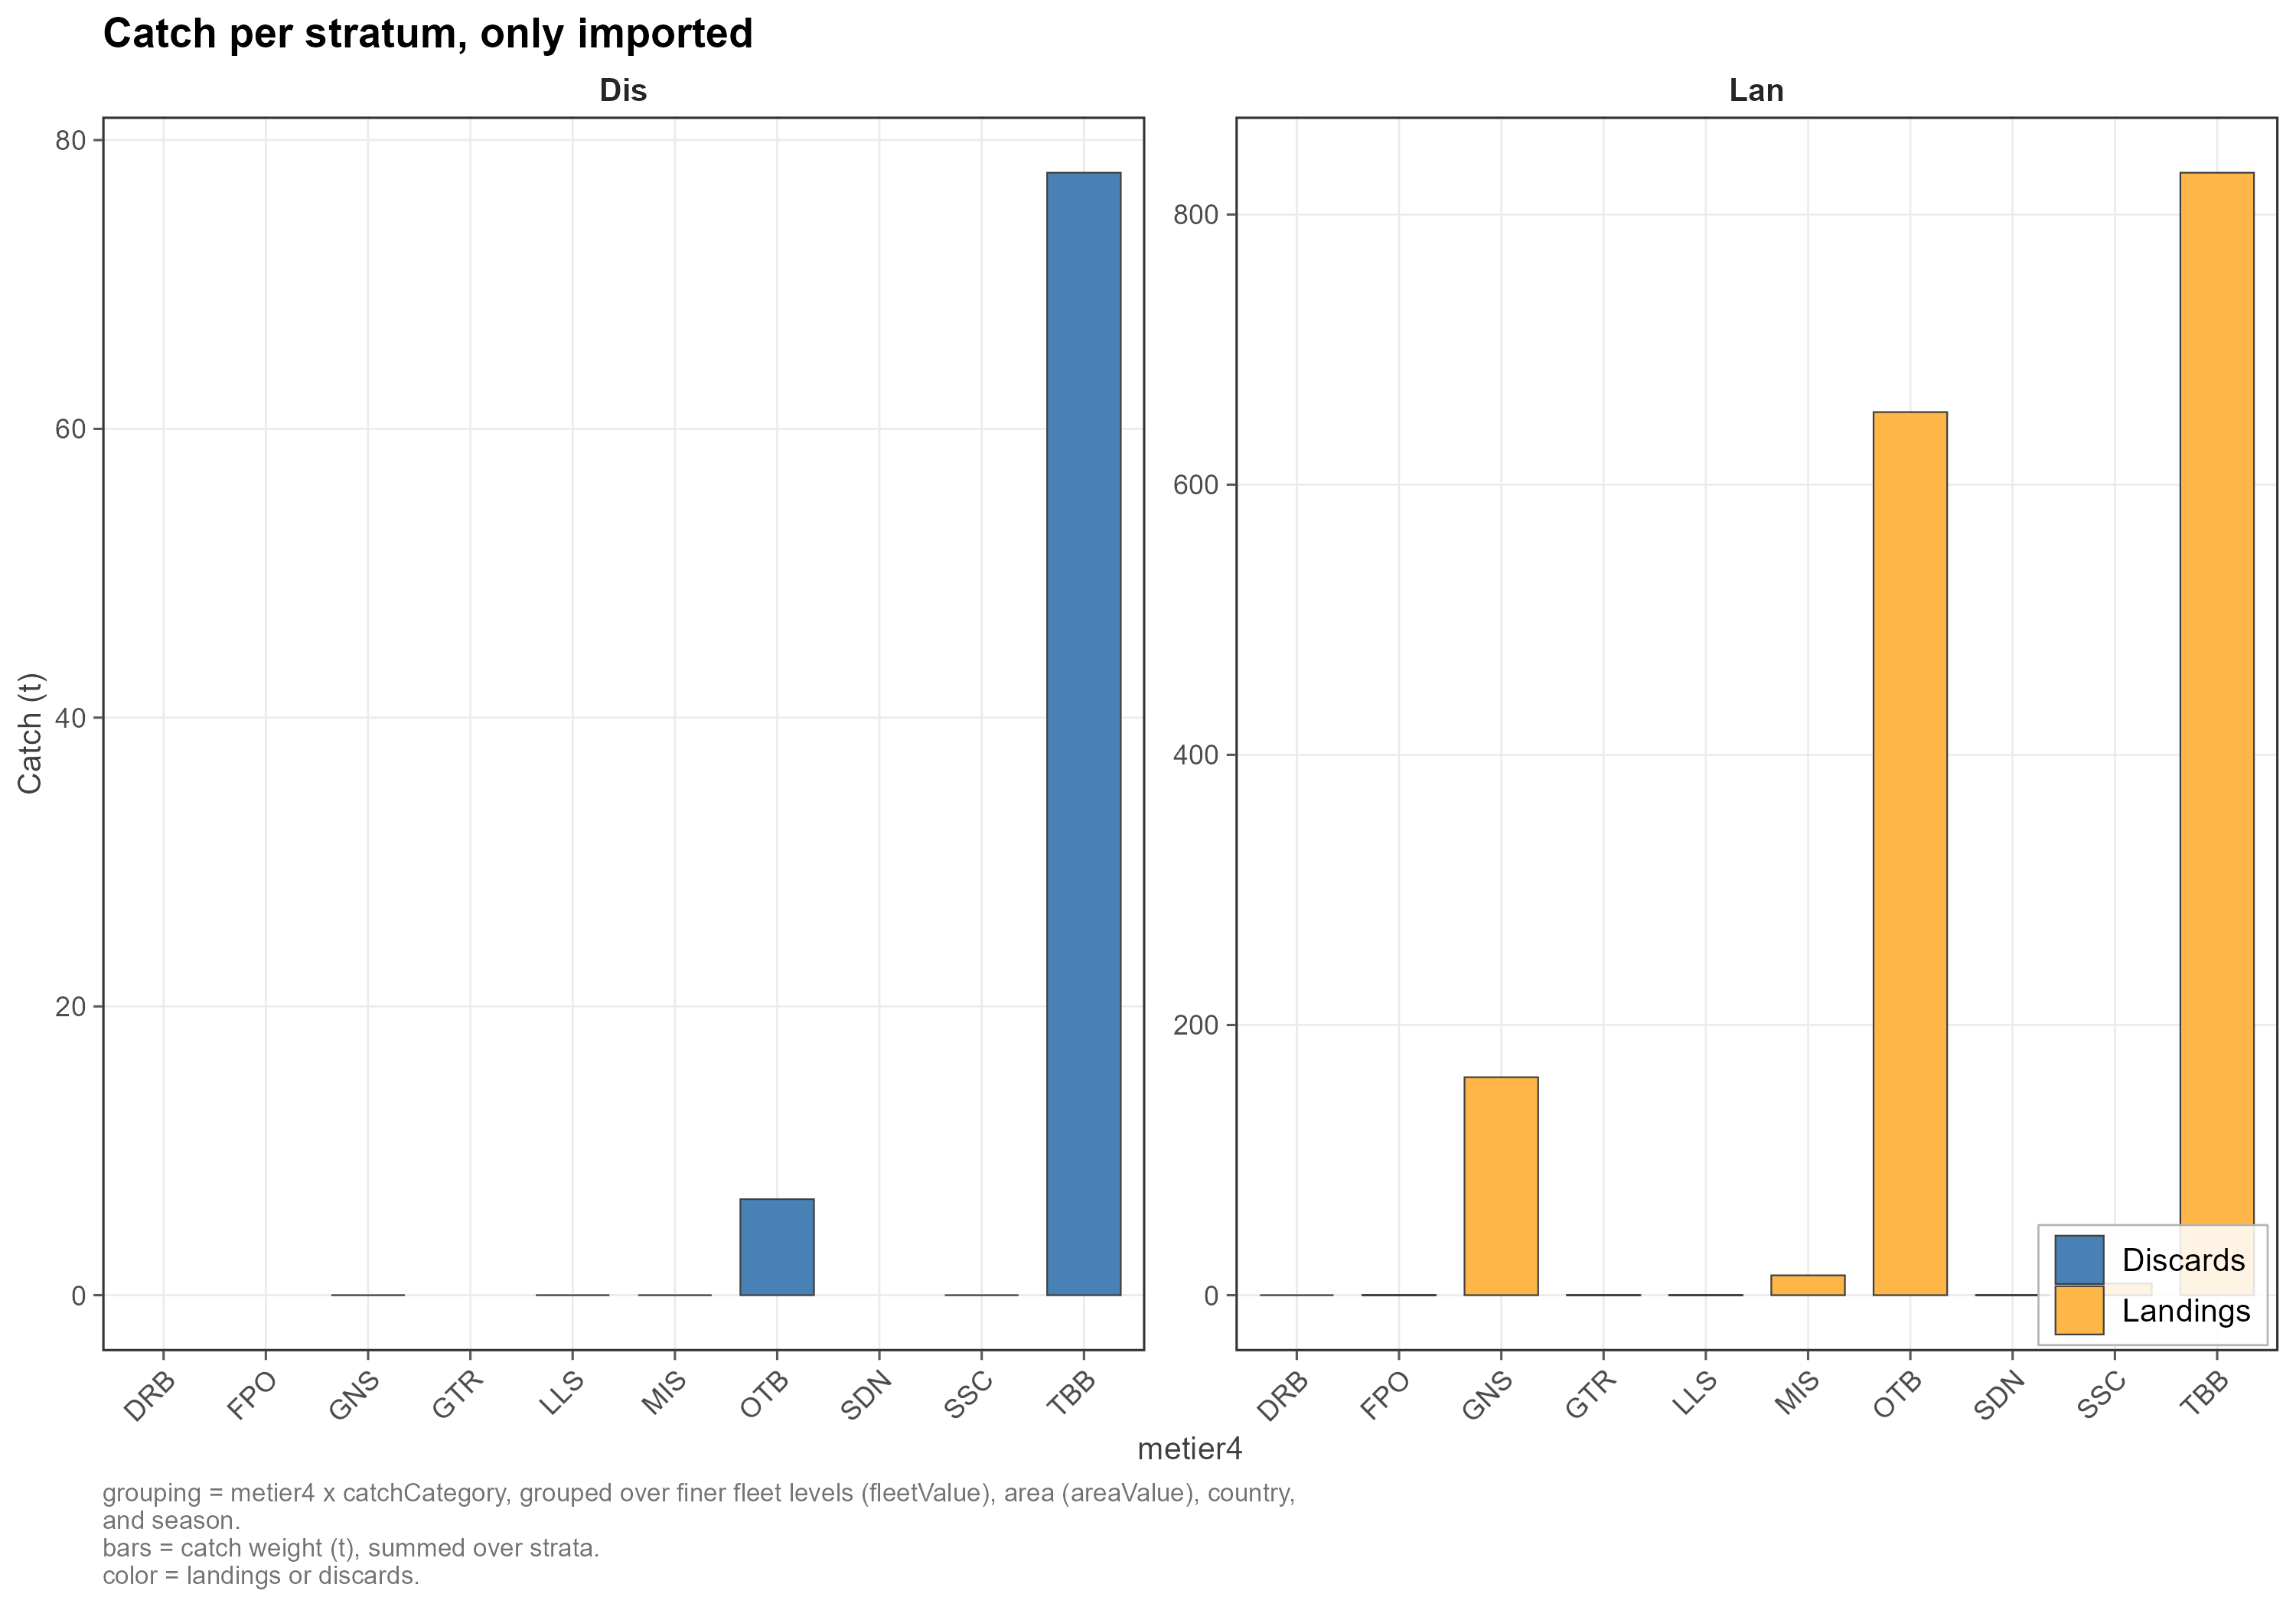
\includegraphics[width=1\linewidth,height=\textheight,keepaspectratio,alt={Two panels, discards and landings in tonnes for each metier; the beam trawls are the largest bar in both, followed by the otter trawls.}]{../../../output/figures/2_discard_raising/discard_raising_01.png}

}

\caption{\label{fig-catch-metier}The catch as reported (only imported):
the weight of the landings and of the discards by metier. File
\texttt{discard\_raising\_01.png}.}

\end{figure}%

\section{Discard raising}\label{discard-raising}

\subsection{How the raising works}\label{how-the-raising-works}

Discards are known only where somebody observed them, so only some of
the strata that land brill have a discard estimate: about three quarters
of the landings are in such strata (Figure~\ref{fig-coverage-metier}).
For the others the discards are \emph{raised}: a landings row without a
discard estimate gets a discards row equal to its landings times a
\textbf{discard ratio} (discards divided by landings), taken from a
group of comparable strata, its donors.

The comparable strata are written down by hand as \textbf{raising
groups}. A group is a pair of conditions on the columns of the catch
table:

\begin{itemize}
\tightlist
\item
  the \textbf{raising strata}: the landings that are raised together. A
  landing is in one group only: \texttt{check\_group\_conditions()}
  stops at a landing that falls in two groups and reports one that falls
  in none;
\item
  the \textbf{matched data}: the strata whose landings and discards give
  the ratio of the group. They are often the raising strata themselves,
  but they can be a wider pool when the group has too little discard
  data of its own, and the pools of different groups may overlap.
\end{itemize}

The ratio is the total discards over the total landings of the donors
that have a discard estimate, so the large strata weigh more. Everything
else is kept as it came. The result of \texttt{catchRaising()} is the
catch table with the raised discards added, each row marked
\texttt{imported} or \texttt{raised} and carrying the name of its group.

\subsection{Looking at the data to define the
groups}\label{looking-at-the-data-to-define-the-groups}

The groups follow what the data say about where discards are observed
and how large they are.

\textbf{Where are discards observed?} The beam trawls and the otter
trawls, which land most of the brill, have most of their landings in
strata with a discard estimate; many small fleets have none
(Figure~\ref{fig-coverage-metier}). Taken by gear group and mesh
(Figure~\ref{fig-coverage-heat}), most of the landings of the beam
trawls (G1), the nets (G2) and the otter trawls (G3) are in tiles with
at least half of the landings covered (green). The rest of the fleets
(G4) are sparsely sampled and need the pool of all the others.

\begin{figure}[htbp]

\centering{

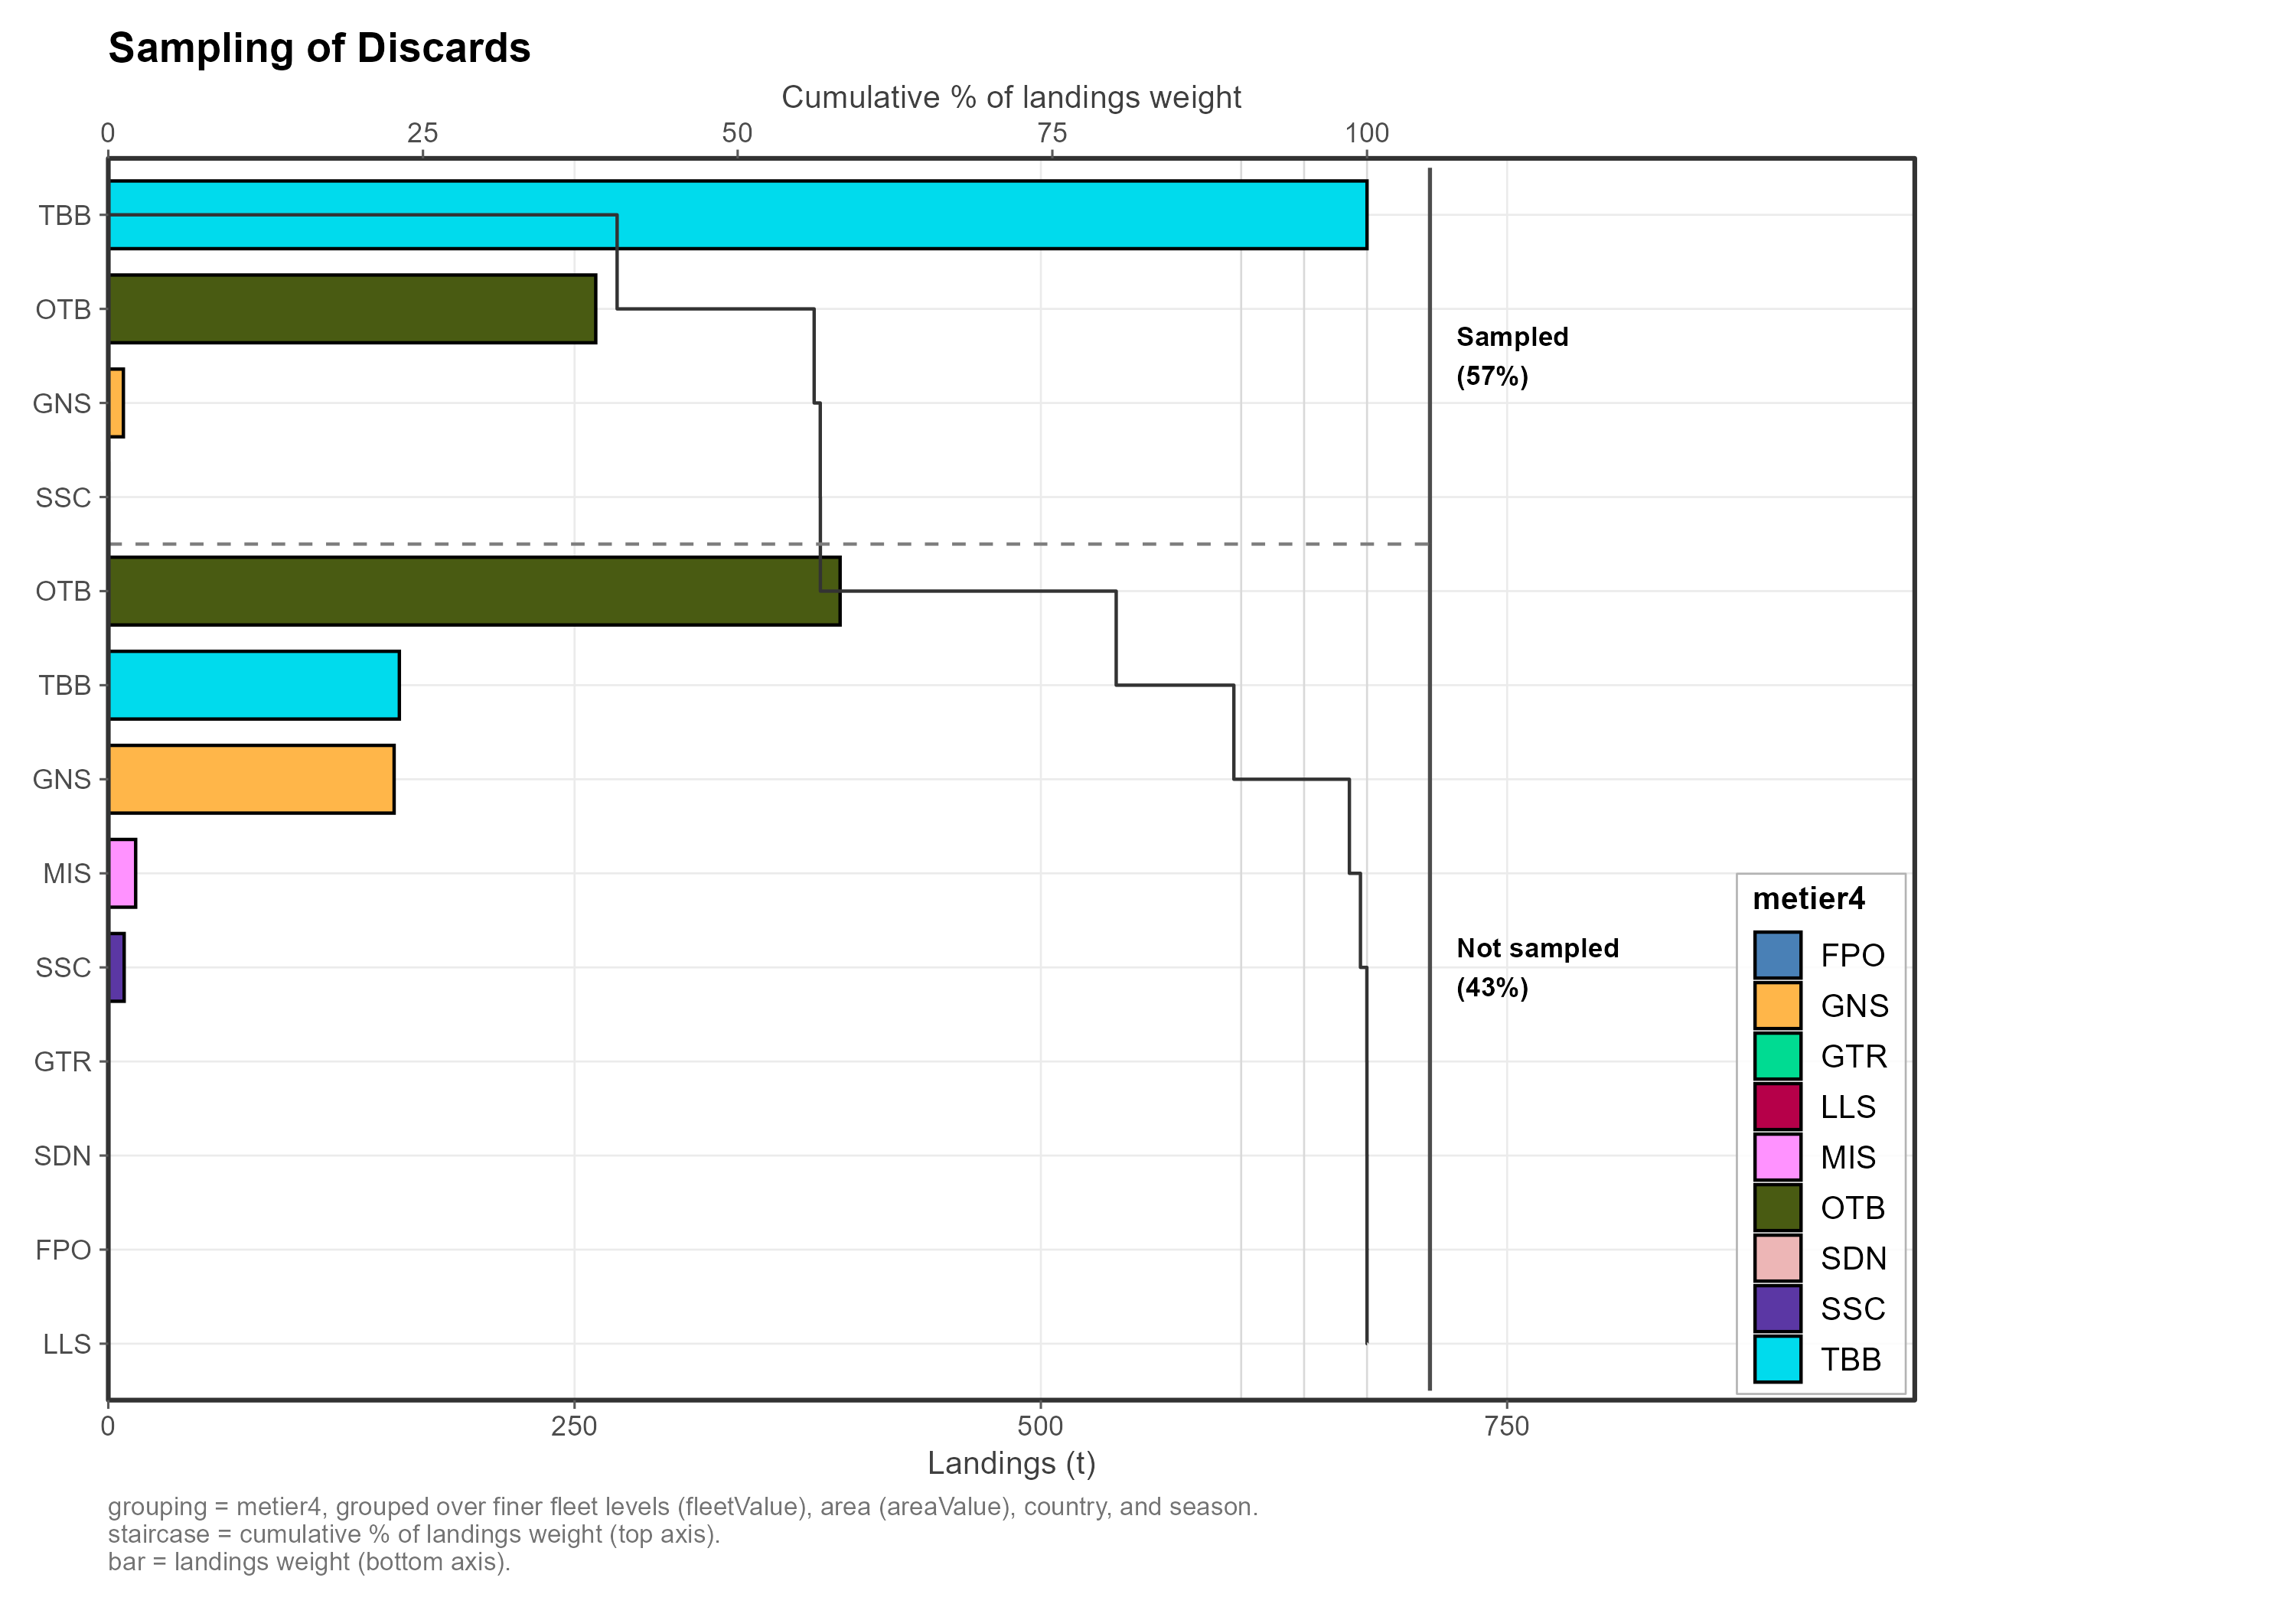
\includegraphics[width=1\linewidth,height=\textheight,keepaspectratio,alt={Horizontal bars of landings by metier, sampled strata above the dashed line and not sampled below, with a staircase of the cumulative share of the landings.}]{../../../output/figures/2_discard_raising/discard_raising_02.png}

}

\caption{\label{fig-coverage-metier}Sampling of the discards by metier:
the landings of each metier (bars, bottom axis) and the cumulative share
of the landings with a discard estimate (staircase, top axis); about
three quarters of the landings are sampled. File
\texttt{discard\_raising\_02.png}.}

\end{figure}%

\begin{figure}[htbp]

\centering{

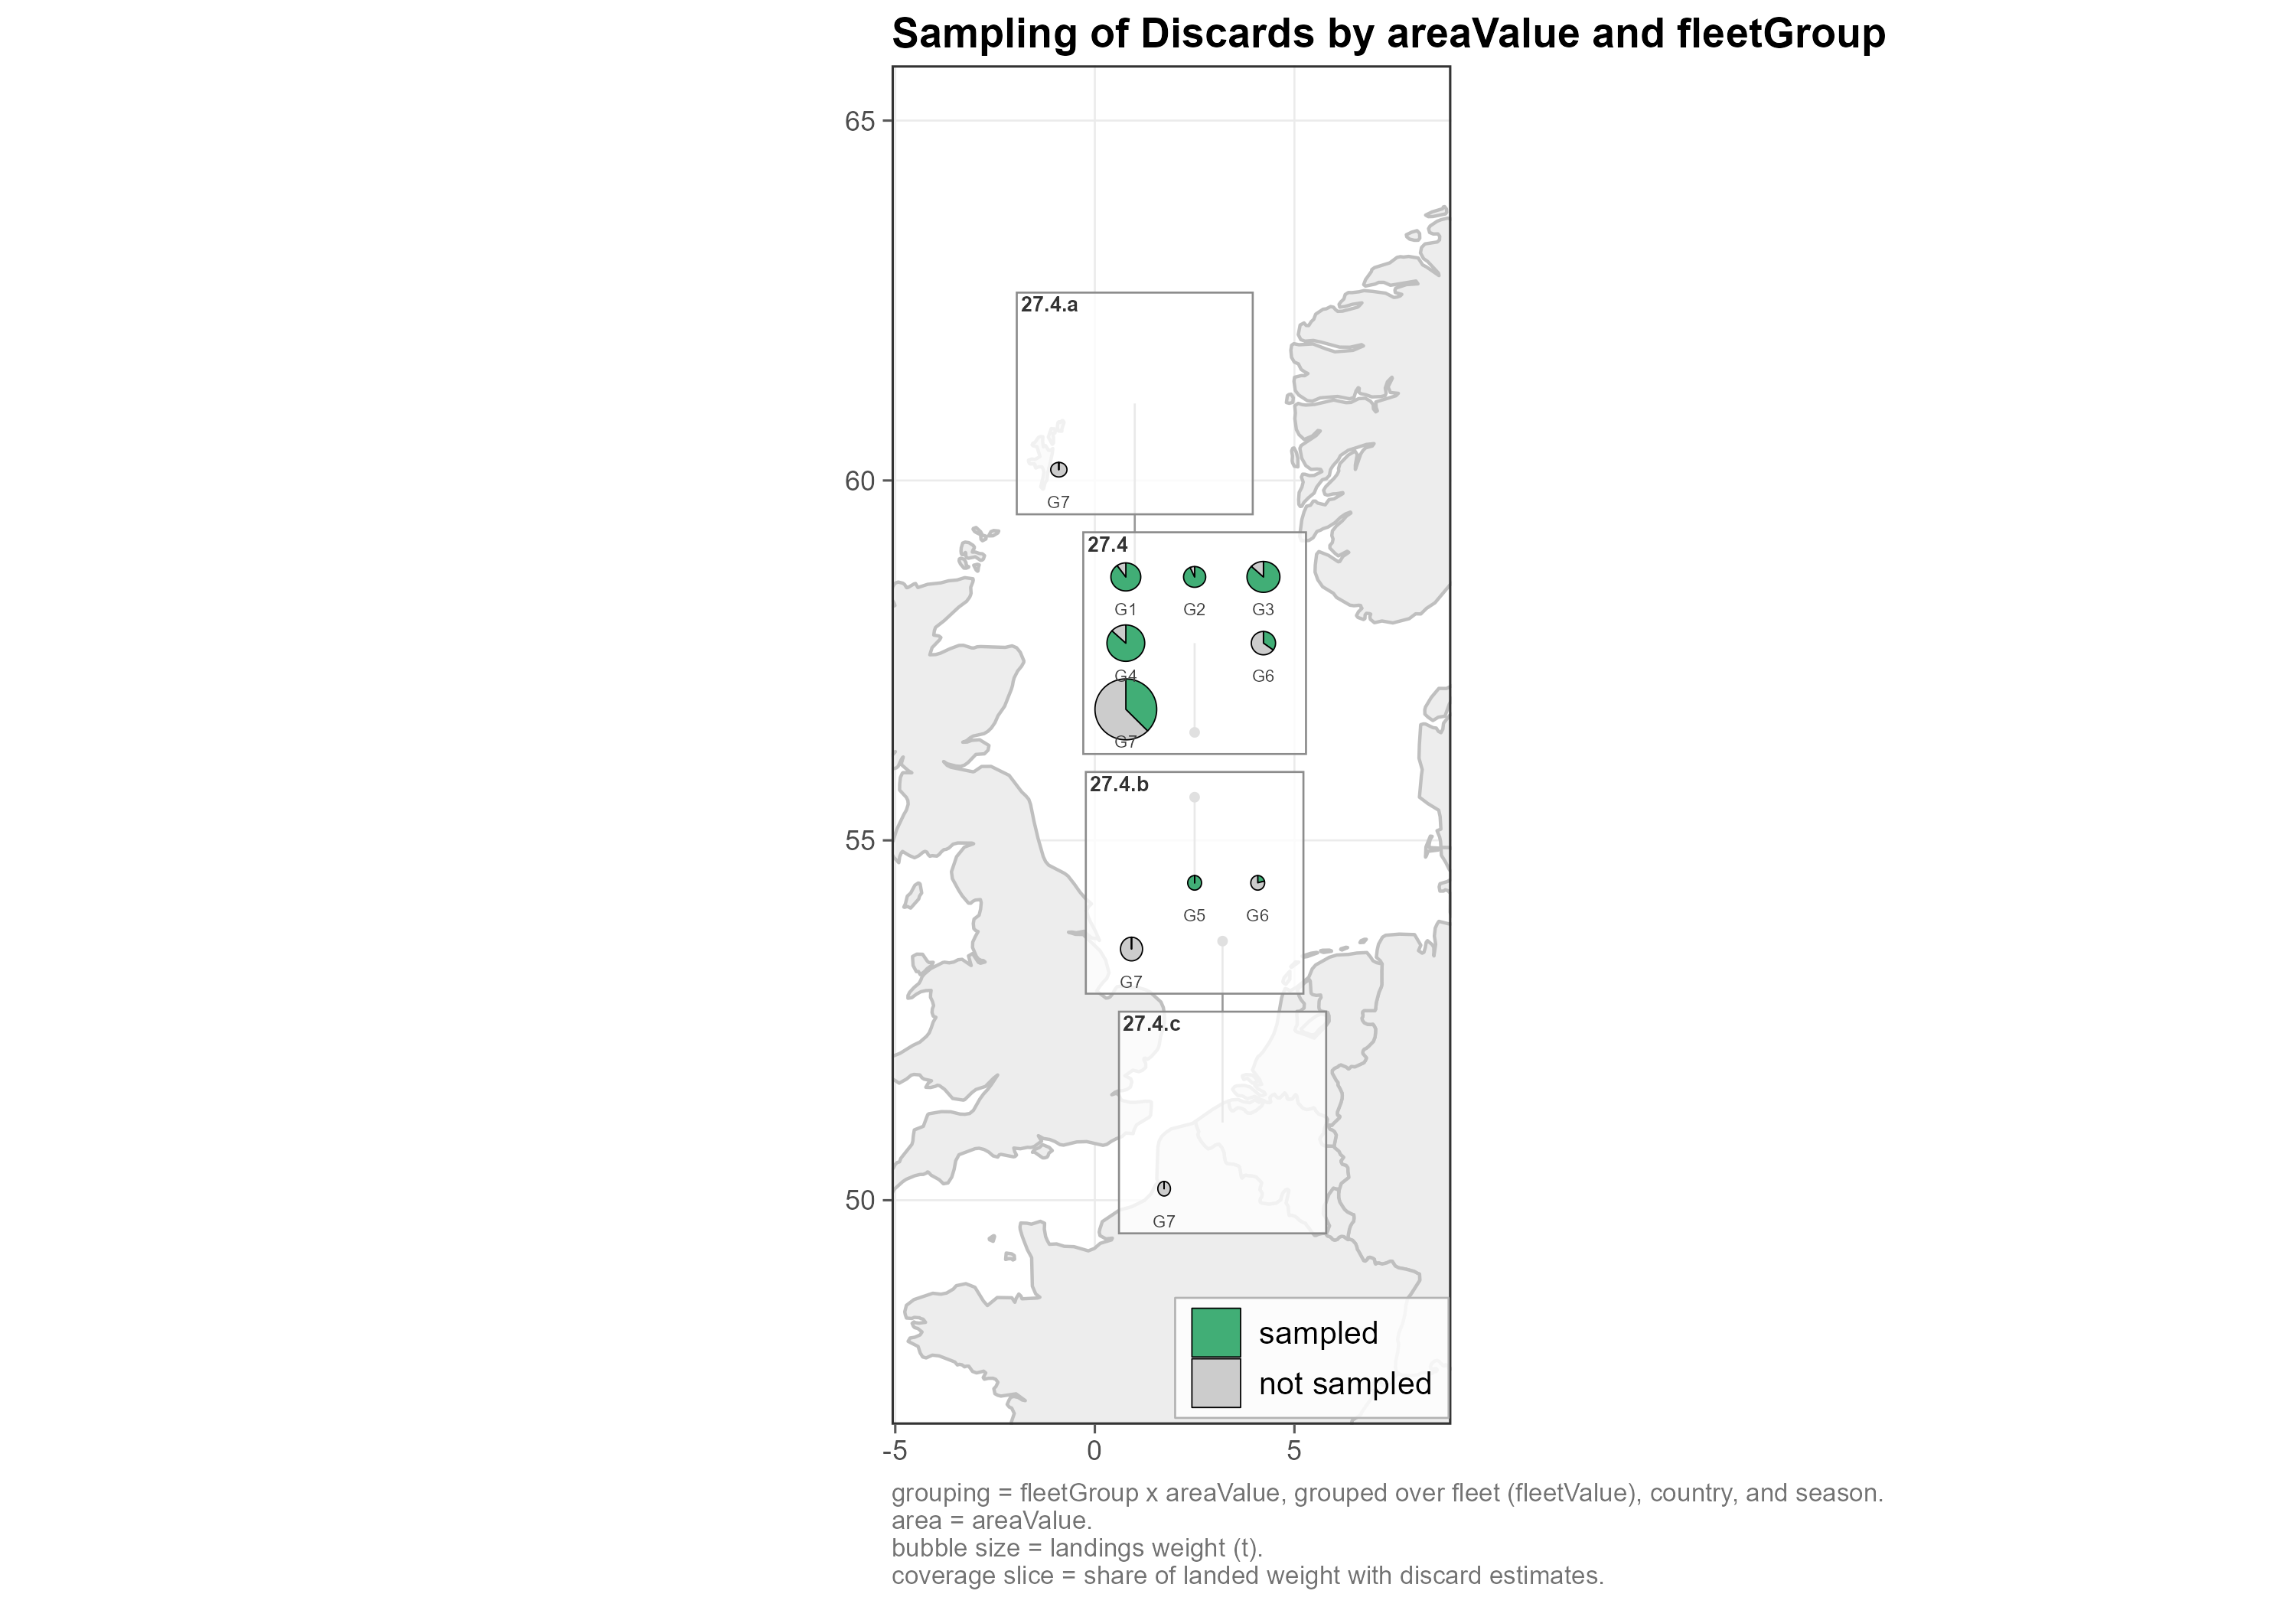
\includegraphics[width=1\linewidth,height=\textheight,keepaspectratio,alt={Four panels, one for each fleet group, of coloured tiles by metier and mesh with the landings in tonnes.}]{../../../output/figures/2_discard_raising/discard_raising_04.png}

}

\caption{\label{fig-coverage-heat}Sampling of the discards by fleet
group, metier and mesh: the share of the landings with a discard
estimate (green: at least 50\%, yellow: less, red: none) and the
landings in tonnes. File \texttt{discard\_raising\_04.png}.}

\end{figure}%

\textbf{How large are they?} The discard ratio of the strata that were
sampled is low and steady for the beam trawls and higher, and more
scattered, for the nets and the otter trawls, where the few strata above
50\% are nearly all in the Kattegat (27.3.a.21)
(Figure~\ref{fig-dr-area}).

\begin{figure}[htbp]

\centering{

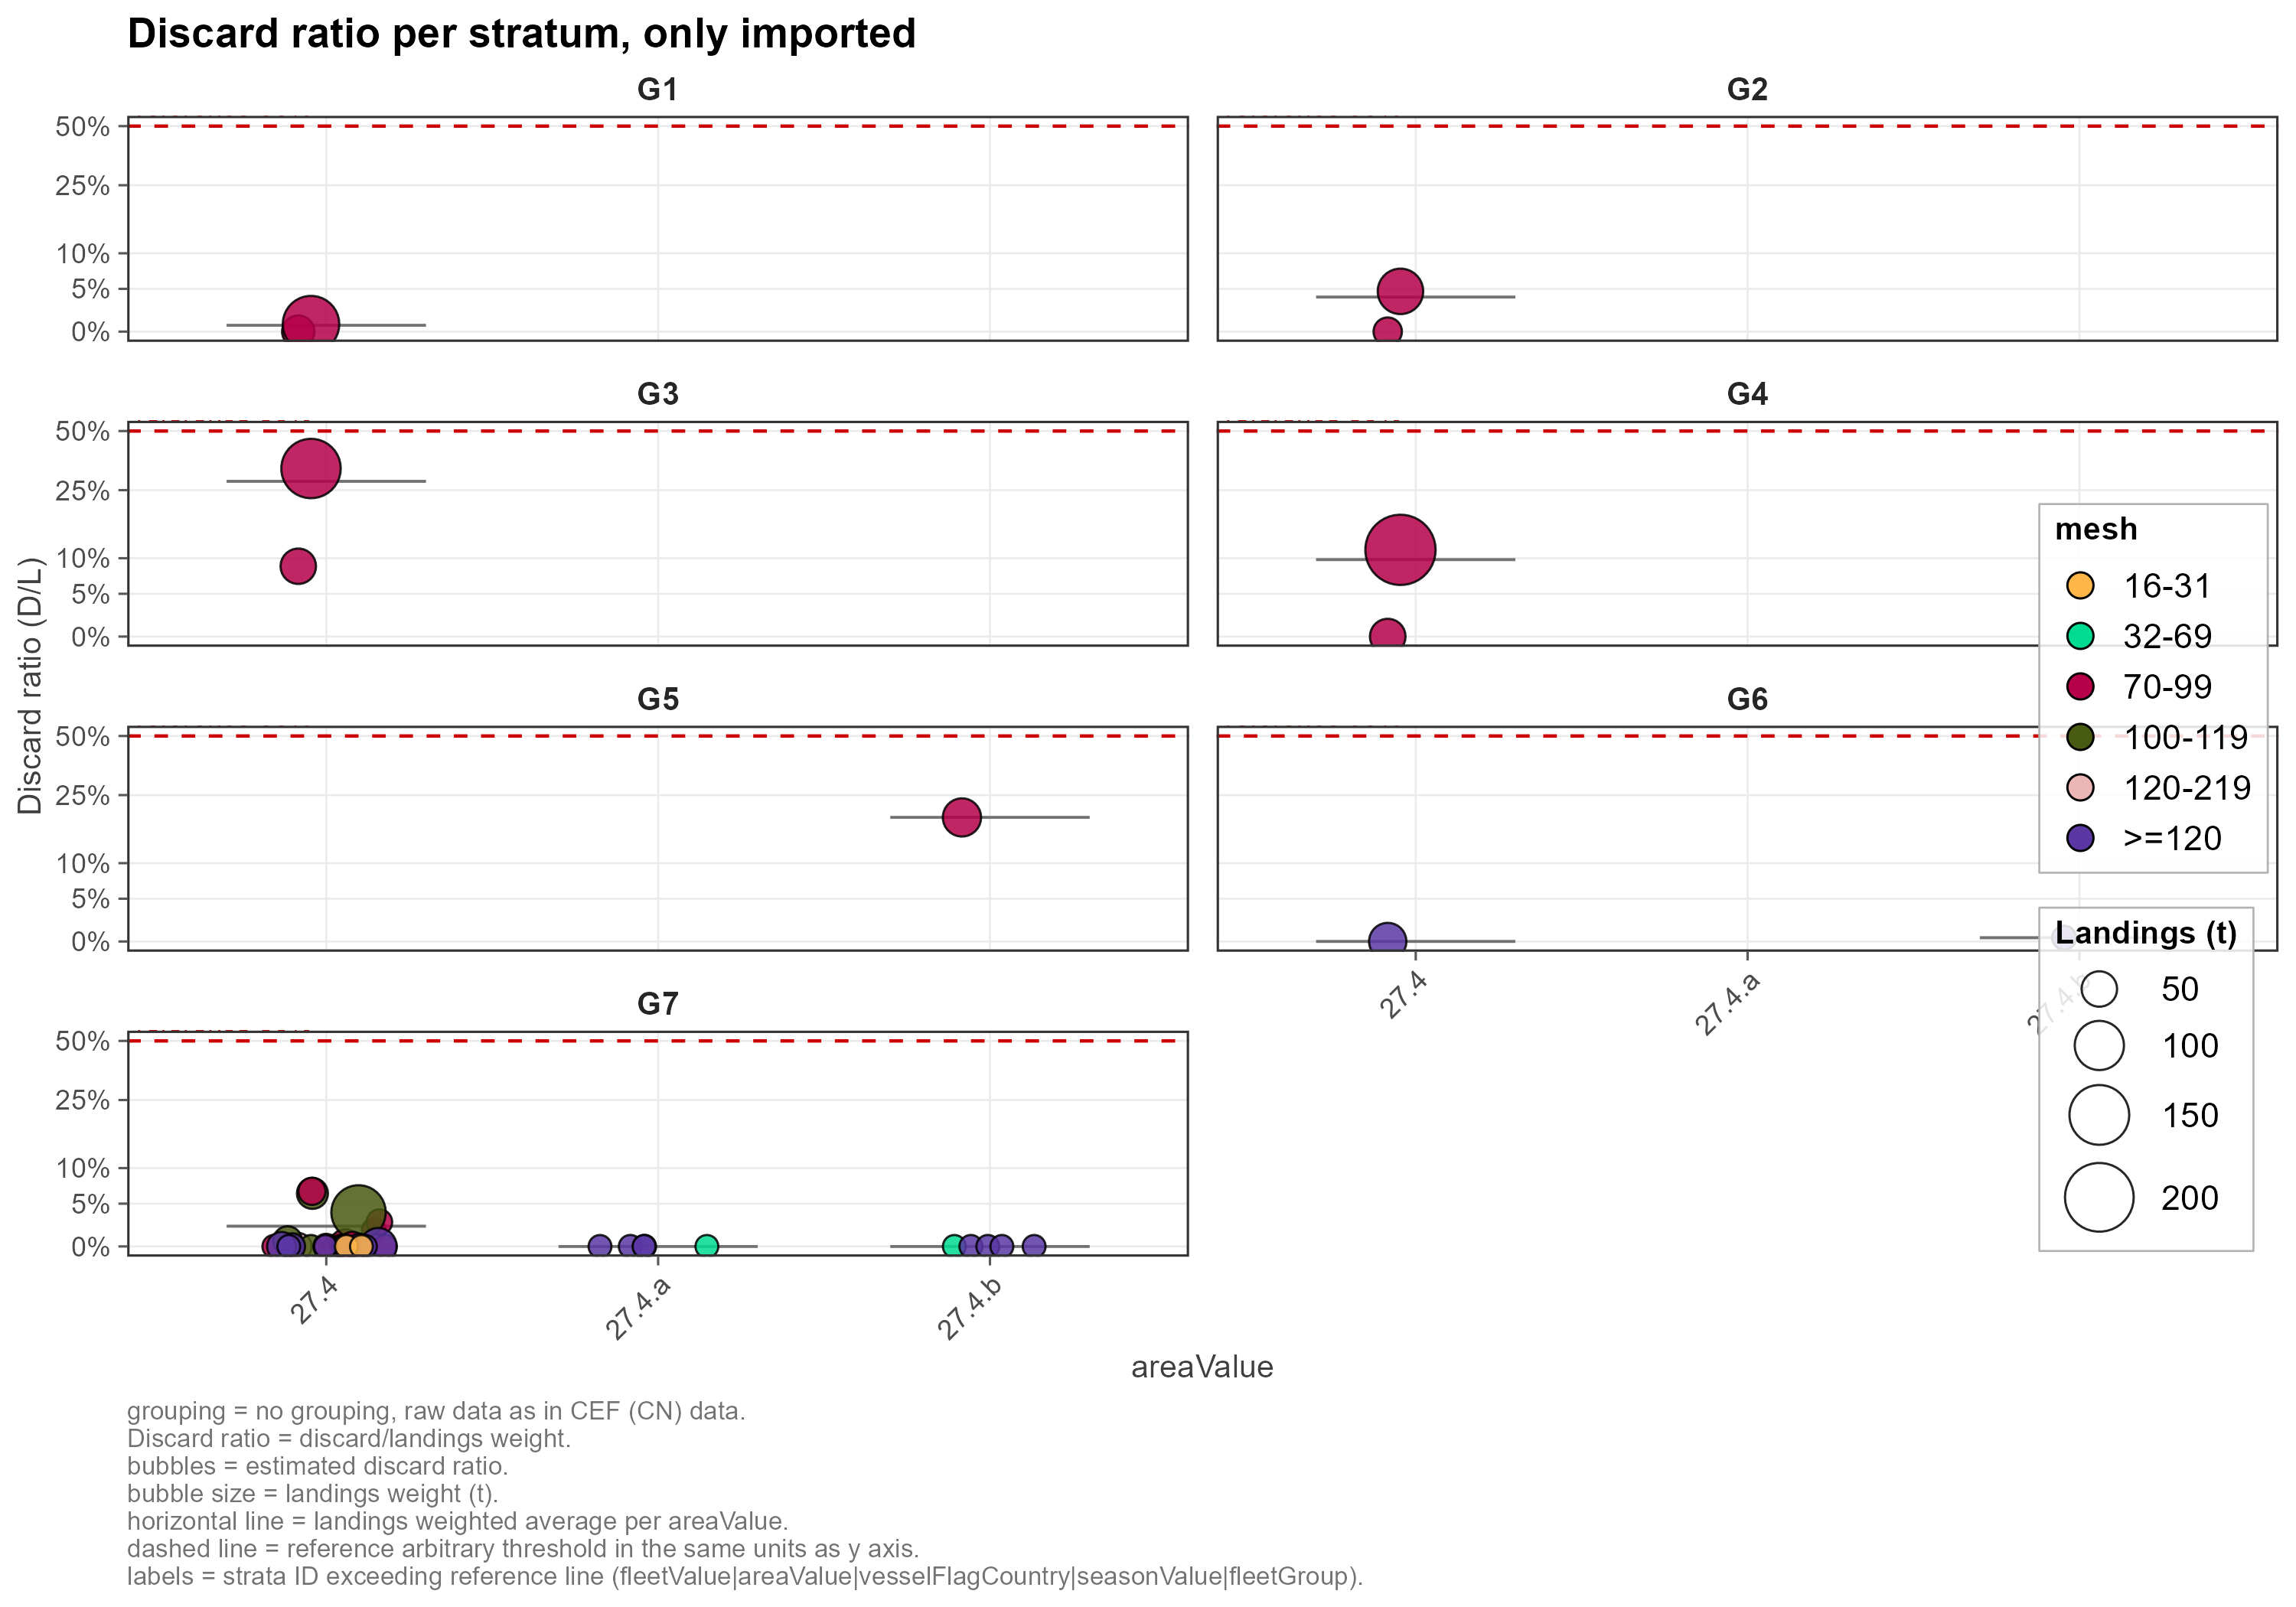
\includegraphics[width=1\linewidth,height=\textheight,keepaspectratio,alt={Four panels of points, the discard ratio by area for each fleet group, with a dashed line at 50\% and a few high points in 27.3.a.21.}]{../../../output/figures/2_discard_raising/discard_raising_06.png}

}

\caption{\label{fig-dr-area}The discard ratio (discards over landings)
of the strata that were sampled, by area, mesh (colour) and fleet group;
the dashed line is 50\%. File \texttt{discard\_raising\_06.png}.}

\end{figure}%

\textbf{What explains them?} The strata were clustered by their discard
rate, and the variables that best predict the cluster are the area, the
mesh and the gear; the season is the weakest
(Figure~\ref{fig-clusters}). Gear is the main axis of the groups, and
the area is what the alternative below adds.

\begin{figure}[htbp]

\centering{

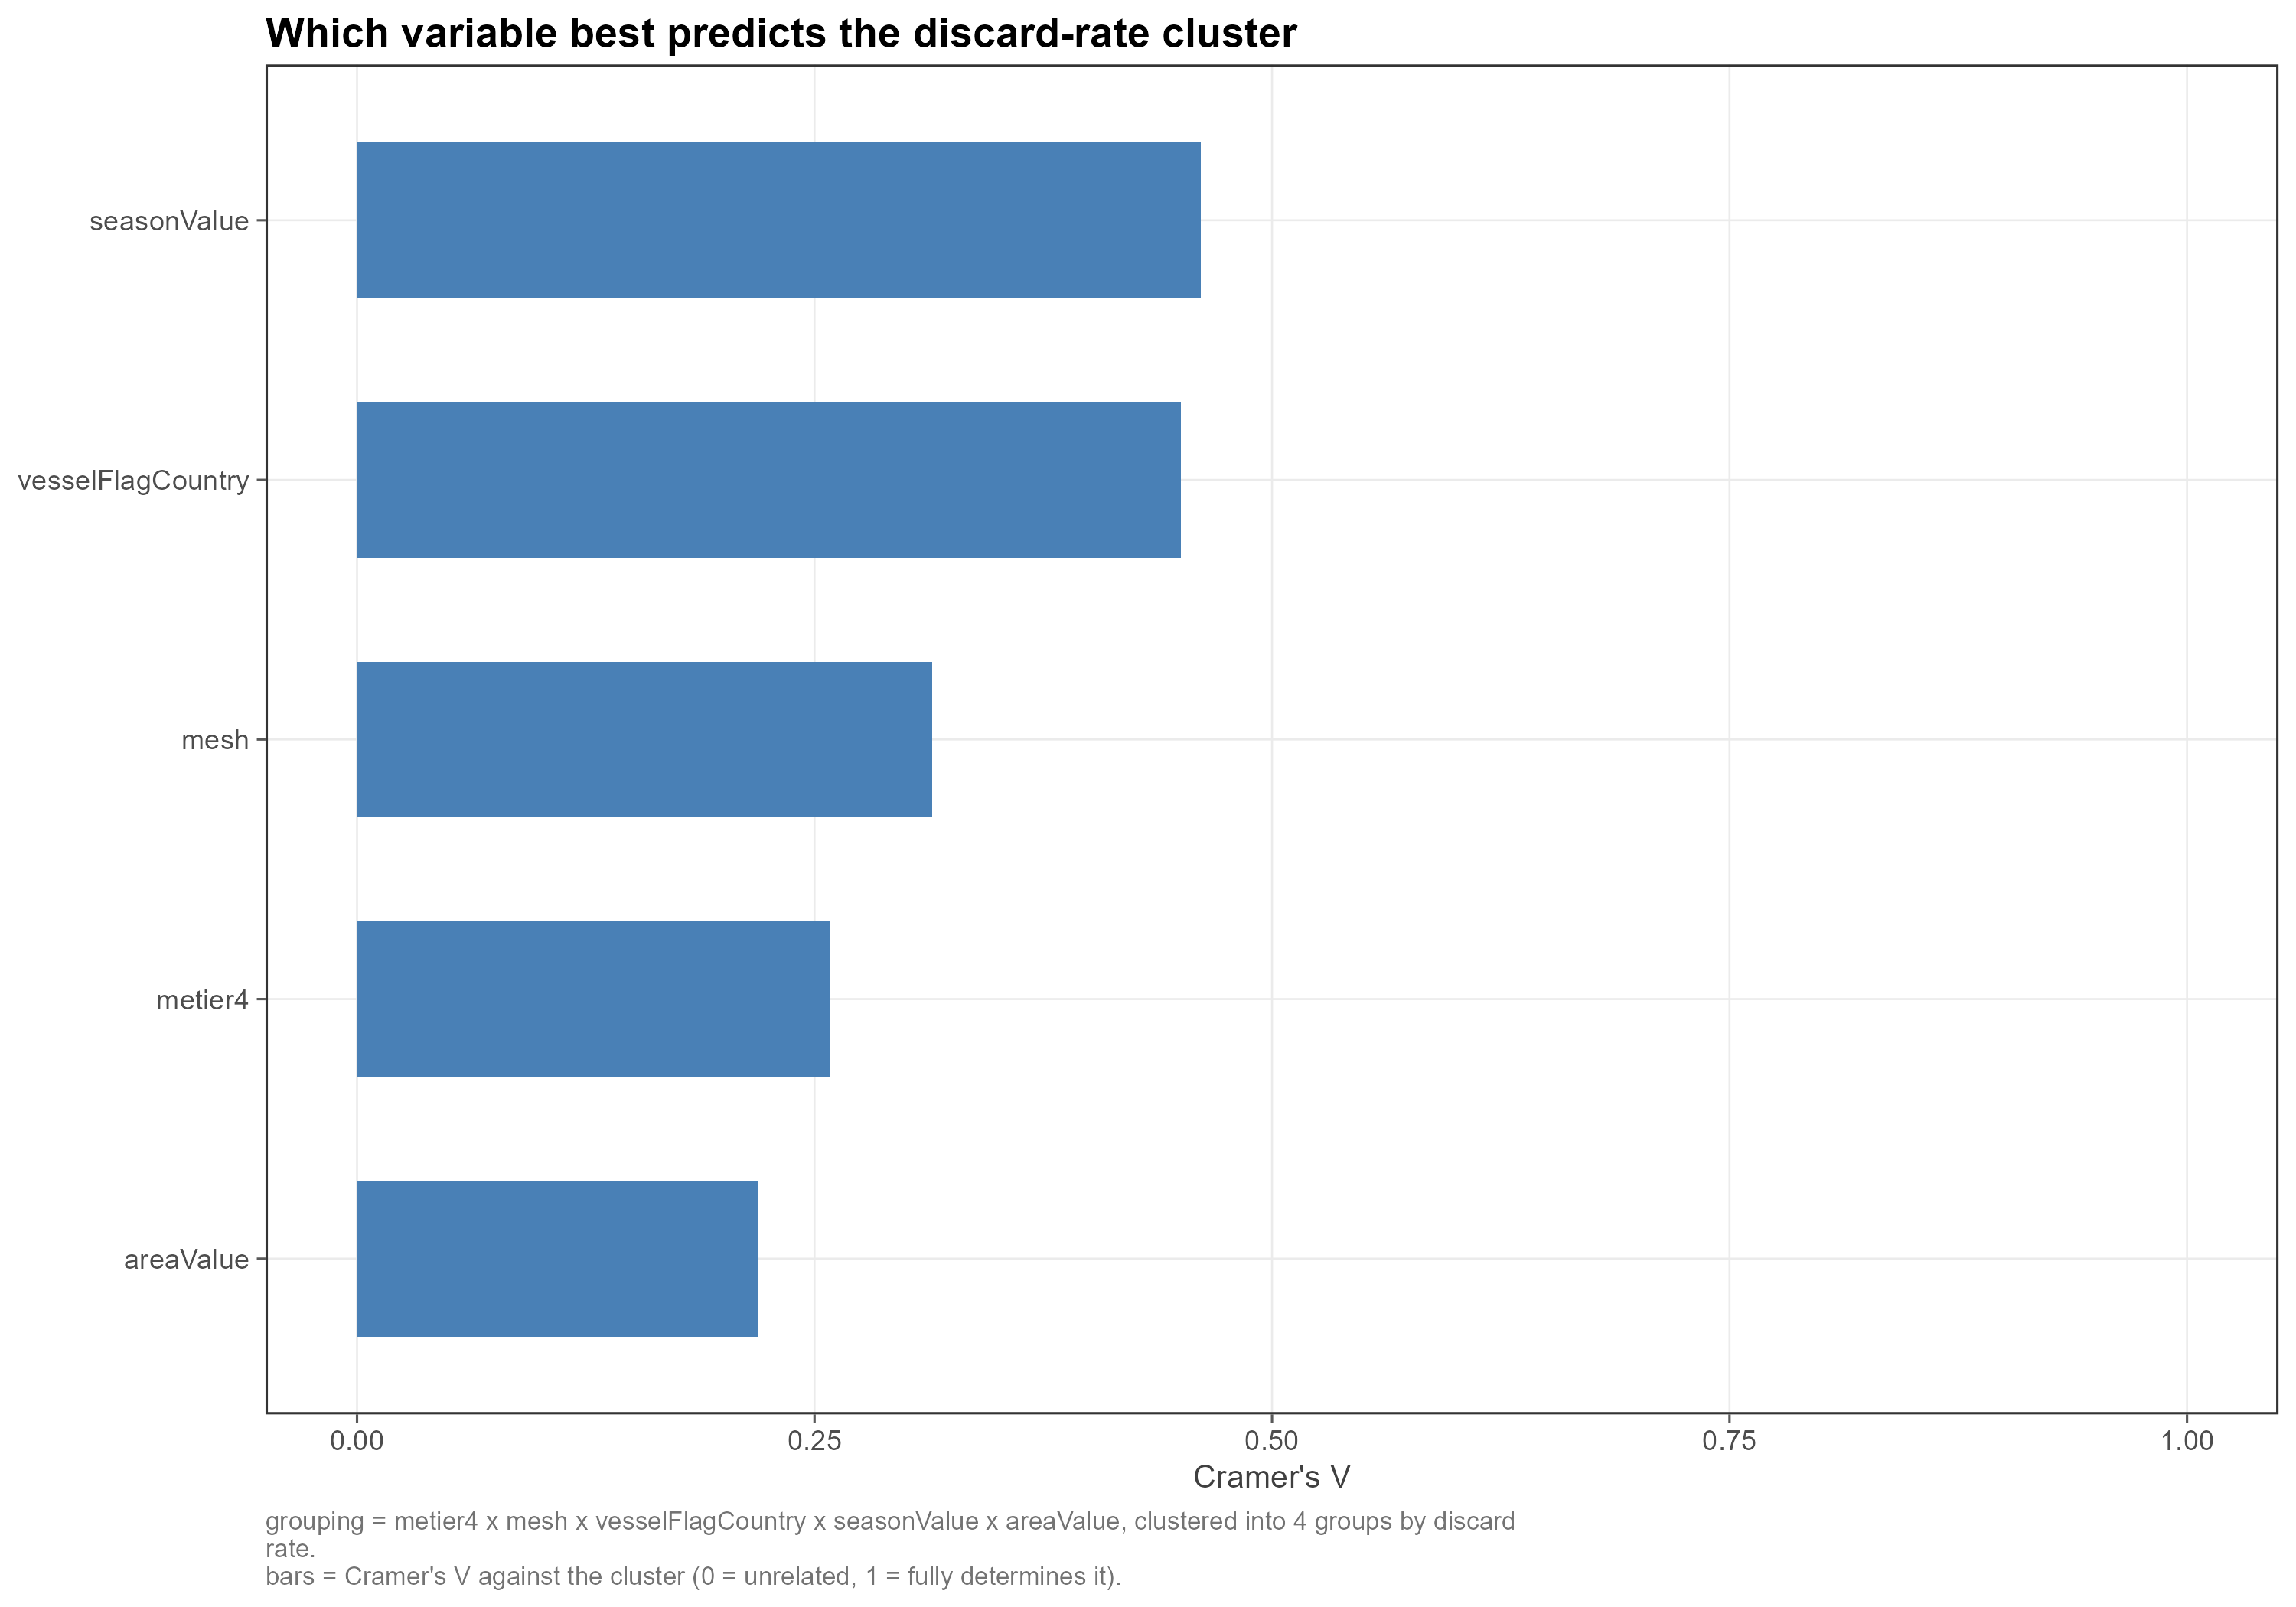
\includegraphics[width=0.85\linewidth,height=\textheight,keepaspectratio,alt={Horizontal bars of Cramer\textquotesingle s V for the area, the mesh, the metier, the country and the season, in decreasing order.}]{../../../output/figures/2_discard_raising/discard_raising_08.png}

}

\caption{\label{fig-clusters}Which variable best predicts the
discard-rate cluster of a stratum (Cramer's V: 0 is unrelated, 1
determines it). File \texttt{discard\_raising\_08.png}.}

\end{figure}%

\subsection{The usual method}\label{the-usual-method}

The usual method has five groups, by gear
(Table~\ref{tbl-groups-usual}). Here is the code of the script,
\texttt{model\_discard\_raising.R}:

\emph{(this code is no longer in the script)}

\emph{(this code is no longer in the script)}

\begin{longtable}[]{@{}
  >{\raggedright\arraybackslash}p{(\linewidth - 6\tabcolsep) * \real{0.2200}}
  >{\raggedright\arraybackslash}p{(\linewidth - 6\tabcolsep) * \real{0.2500}}
  >{\raggedright\arraybackslash}p{(\linewidth - 6\tabcolsep) * \real{0.2700}}
  >{\raggedright\arraybackslash}p{(\linewidth - 6\tabcolsep) * \real{0.2600}}@{}}

\caption{\label{tbl-groups-usual}The five groups of the usual method.}

\tabularnewline

\toprule\noalign{}
\begin{minipage}[b]{\linewidth}\raggedright
Group
\end{minipage} & \begin{minipage}[b]{\linewidth}\raggedright
Raising strata
\end{minipage} & \begin{minipage}[b]{\linewidth}\raggedright
Donors
\end{minipage} & \begin{minipage}[b]{\linewidth}\raggedright
Why
\end{minipage} \\
\midrule\noalign{}
\endhead
\bottomrule\noalign{}
\endlastfoot
G1\_TBB & Beam trawls (TBB) & The same strata & Well sampled; a low and
steady ratio. \\
G2\_GTR\_GNS & Gillnets and trammel nets (GNS, GTR) & The same strata &
Sampled in part; the ratio differs from the others. \\
G3\_OTB\_SSC\_SDN & Otter trawls and seines (OTB, SSC, SDN) & The same
strata & Well sampled in part; the ratio varies with area and mesh. \\
G4\_REST & All other metiers (dredges, pots, lines, unclassified),
except the incidental bycatch fleet & All strata but the incidental
bycatch, minus the strata whose own discard ratio is above 50\% (the MIS
metier excepted) & Too little discard data of its own: it draws on all
the fleets, without the strata that look implausible. \\
G5\_IBC & The incidental bycatch fleet (\texttt{MIS\_MIS\_0\_0\_0\_IBC})
& The same strata & No landings: there is nothing to raise. \\

\end{longtable}

The raising adds 23.4 t of discards to the 84.4 t that were reported,
107.8 t in all, of which 22\% is raised (Table~\ref{tbl-raising-usual}).
The ratios the raised discards used are in the last column;
Figure~\ref{fig-dr-usual} shows them as crosses among the imported
strata of their group.

\begin{longtable}[]{@{}
  >{\raggedright\arraybackslash}p{(\linewidth - 10\tabcolsep) * \real{0.2400}}
  >{\raggedleft\arraybackslash}p{(\linewidth - 10\tabcolsep) * \real{0.1300}}
  >{\raggedleft\arraybackslash}p{(\linewidth - 10\tabcolsep) * \real{0.1700}}
  >{\raggedleft\arraybackslash}p{(\linewidth - 10\tabcolsep) * \real{0.1600}}
  >{\raggedleft\arraybackslash}p{(\linewidth - 10\tabcolsep) * \real{0.1500}}
  >{\raggedleft\arraybackslash}p{(\linewidth - 10\tabcolsep) * \real{0.1500}}@{}}

\caption{\label{tbl-raising-usual}The usual method by group: the
landings, the share of the landings whose discard domain has a discard
estimate of the working group, the discards imported and raised (tonnes)
and the discard ratio the raised discards used.}

\tabularnewline

\toprule\noalign{}
\begin{minipage}[b]{\linewidth}\raggedright
Group
\end{minipage} & \begin{minipage}[b]{\linewidth}\raggedleft
Landings (t)
\end{minipage} & \begin{minipage}[b]{\linewidth}\raggedleft
With a discard estimate (\%)
\end{minipage} & \begin{minipage}[b]{\linewidth}\raggedleft
Discards imported (t)
\end{minipage} & \begin{minipage}[b]{\linewidth}\raggedleft
Discards raised (t)
\end{minipage} & \begin{minipage}[b]{\linewidth}\raggedleft
Ratio used (\%)
\end{minipage} \\
\midrule\noalign{}
\endhead
\bottomrule\noalign{}
\endlastfoot
G1 & 151.5 & 90 & 1.0 & 0.1 & 0.7 \\
G2 & 83.1 & 93 & 3.1 & 0.2 & 4.0 \\
G3 & 183.9 & 87 & 44.5 & 6.7 & 27.8 \\
G4 & 255.2 & 87 & 21.7 & 3.3 & 9.8 \\
G5 & 39.7 & 100 & 7.5 & 0.0 & - \\
G6 & 116.0 & 34 & 0.0 & 0.0 & 0.0 \\
G7 & 840.2 & 32 & 6.6 & 13.1 & 2.3 \\
Total & 1,669.5 & 56 & 84.4 & 23.4 & - \\

\end{longtable}

The 24 raised rows of G5 have no donor and raise to nothing.

\begin{figure}[htbp]

\centering{

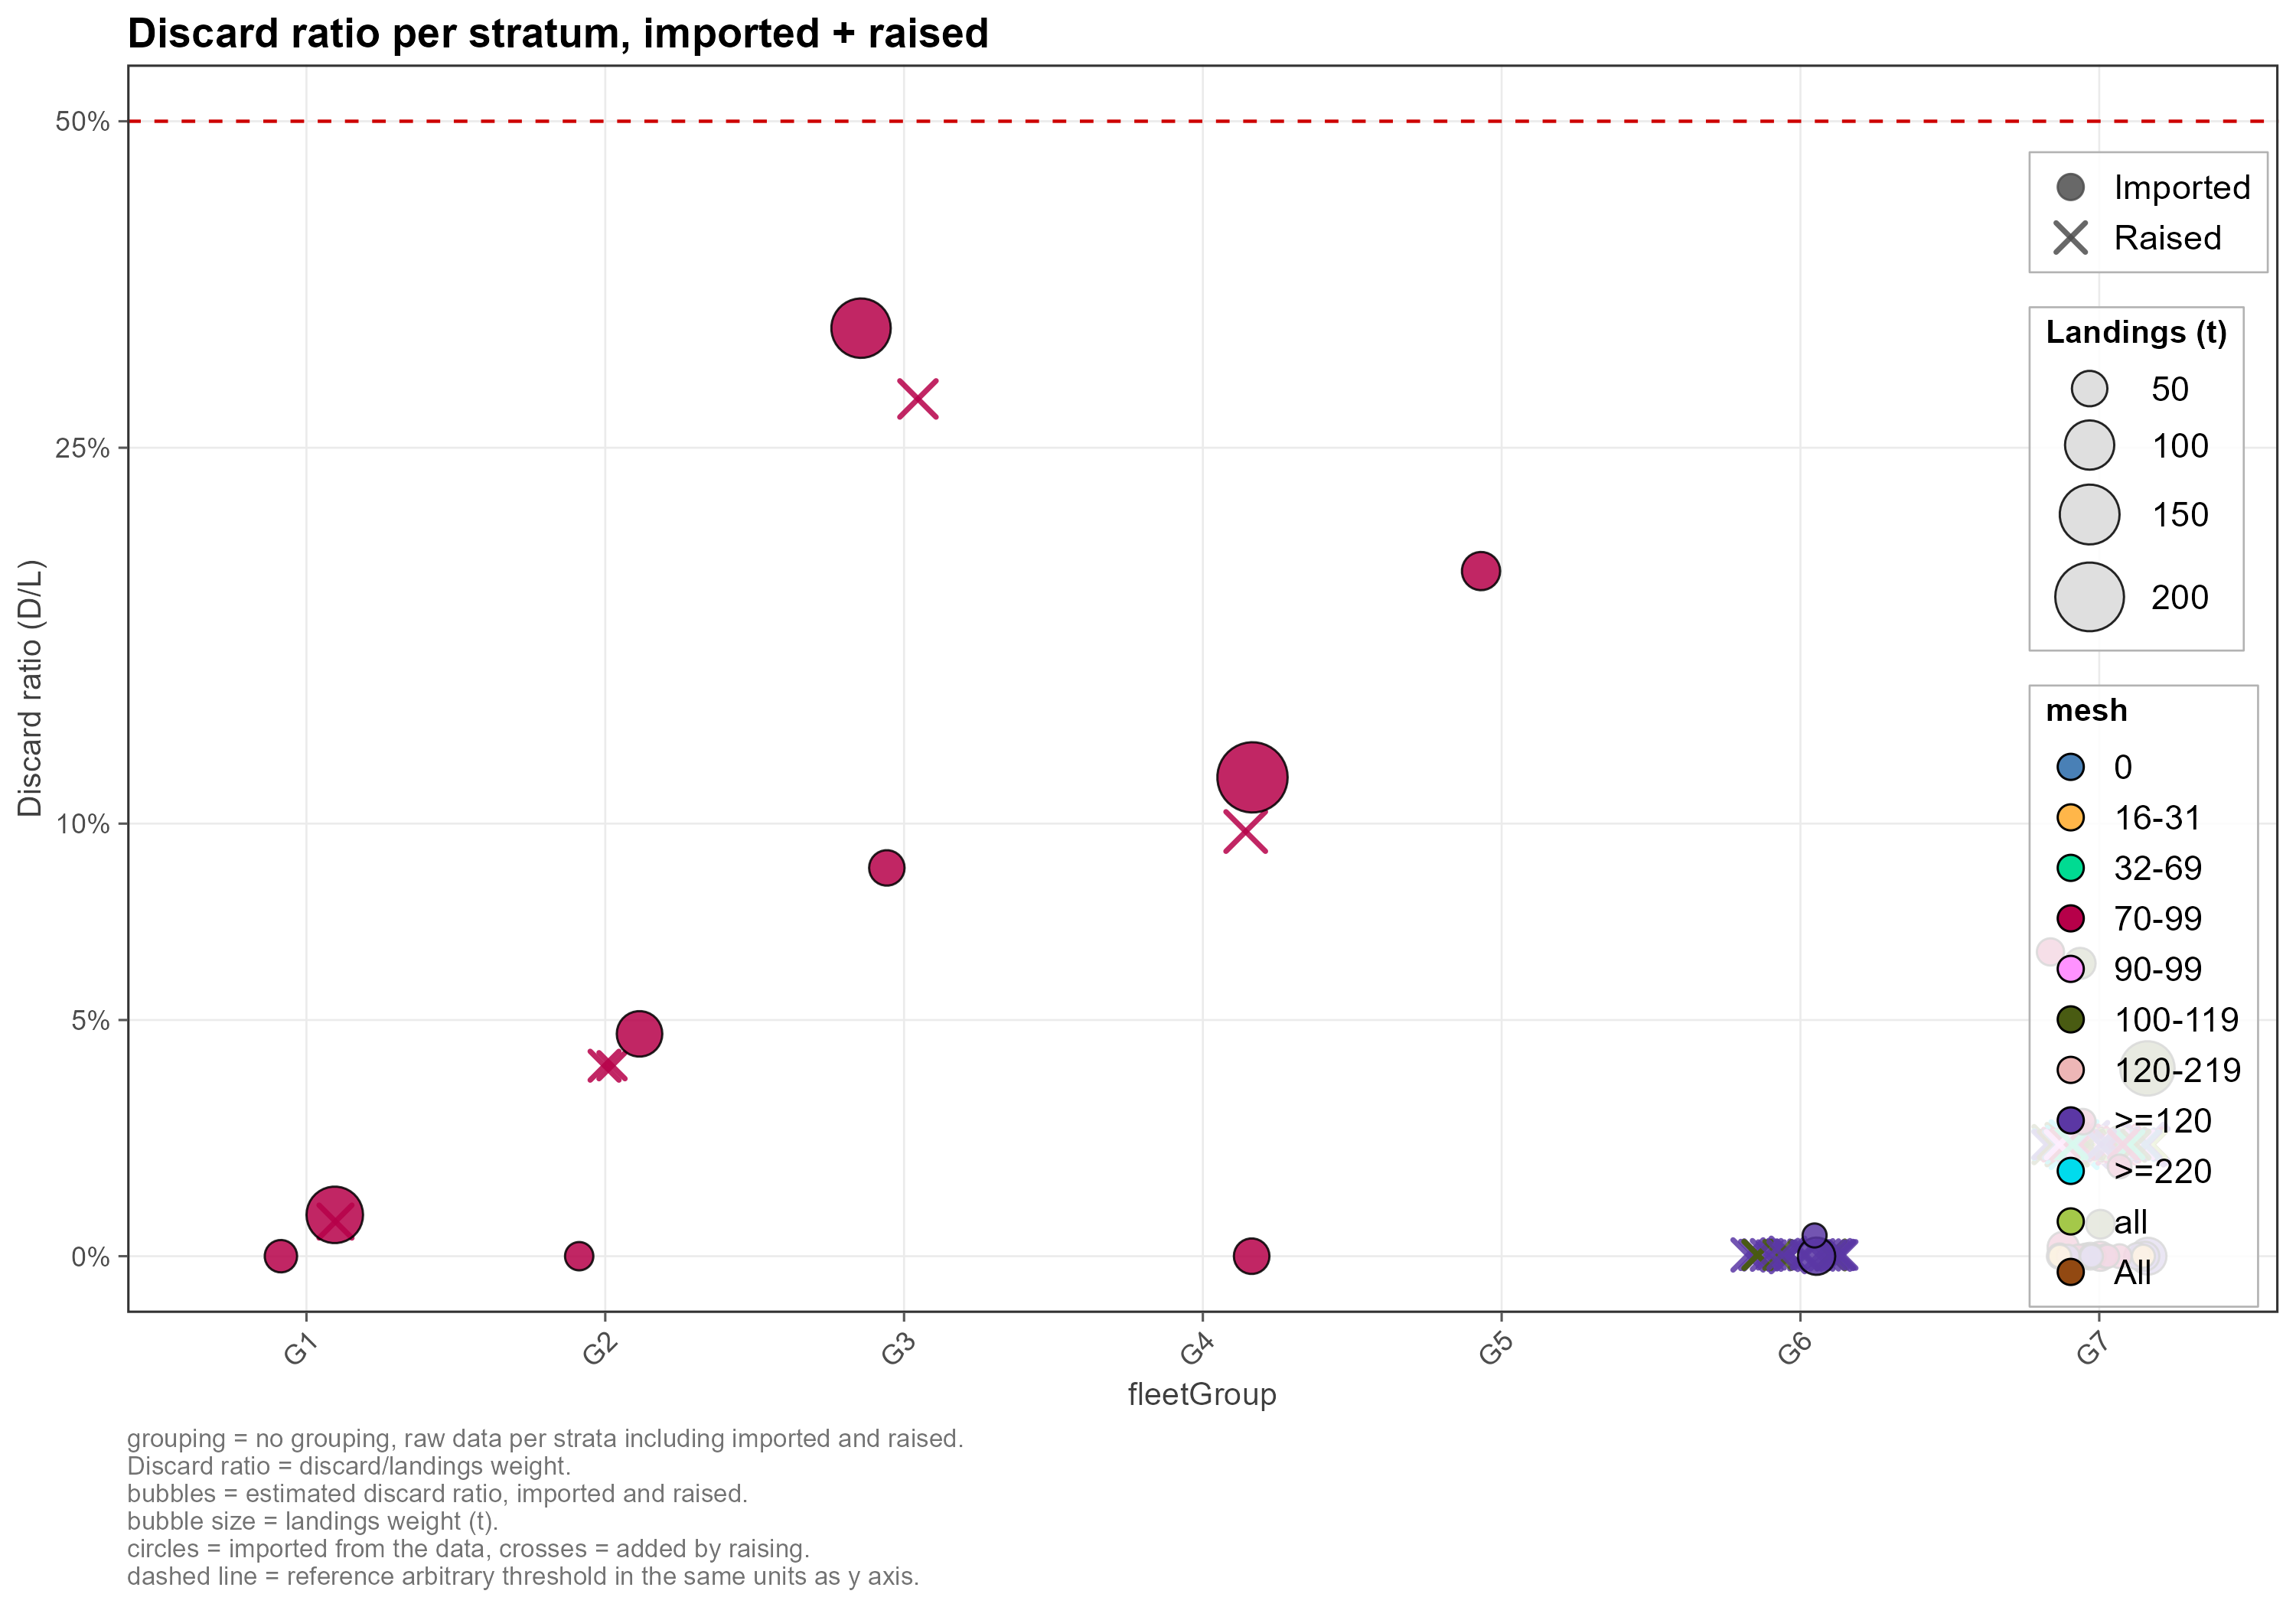
\includegraphics[width=1\linewidth,height=\textheight,keepaspectratio,alt={Points of the discard ratio for each fleet group; the raised strata form horizontal rows of crosses at the ratio of their group.}]{../../../output/figures/2_discard_raising/discard_raising_09.png}

}

\caption{\label{fig-dr-usual}The discard ratio of every stratum after
the usual raising, by group: circles are imported strata, crosses the
raised ones. File \texttt{discard\_raising\_09.png}.}

\end{figure}%

\subsection{The alternative: the Kattegat on its
own}\label{the-alternative-the-kattegat-on-its-own}

The discard ratios of the nets and the otter trawls in the Kattegat
(27.3.a.21) are much higher than elsewhere (Figure~\ref{fig-dr-area}),
and these fleets are well sampled there
(Figure~\ref{fig-coverage-3a21}). In the alternative, called \emph{usual
method with 3.a.21}, the Kattegat strata of G2 and G3 are groups of
their own, G2b and G3b, raised from the strata of the same gears in
27.3.a.21 only; the other groups are those of the usual method
(Table~\ref{tbl-groups-alt}).

\begin{figure}[htbp]

\centering{

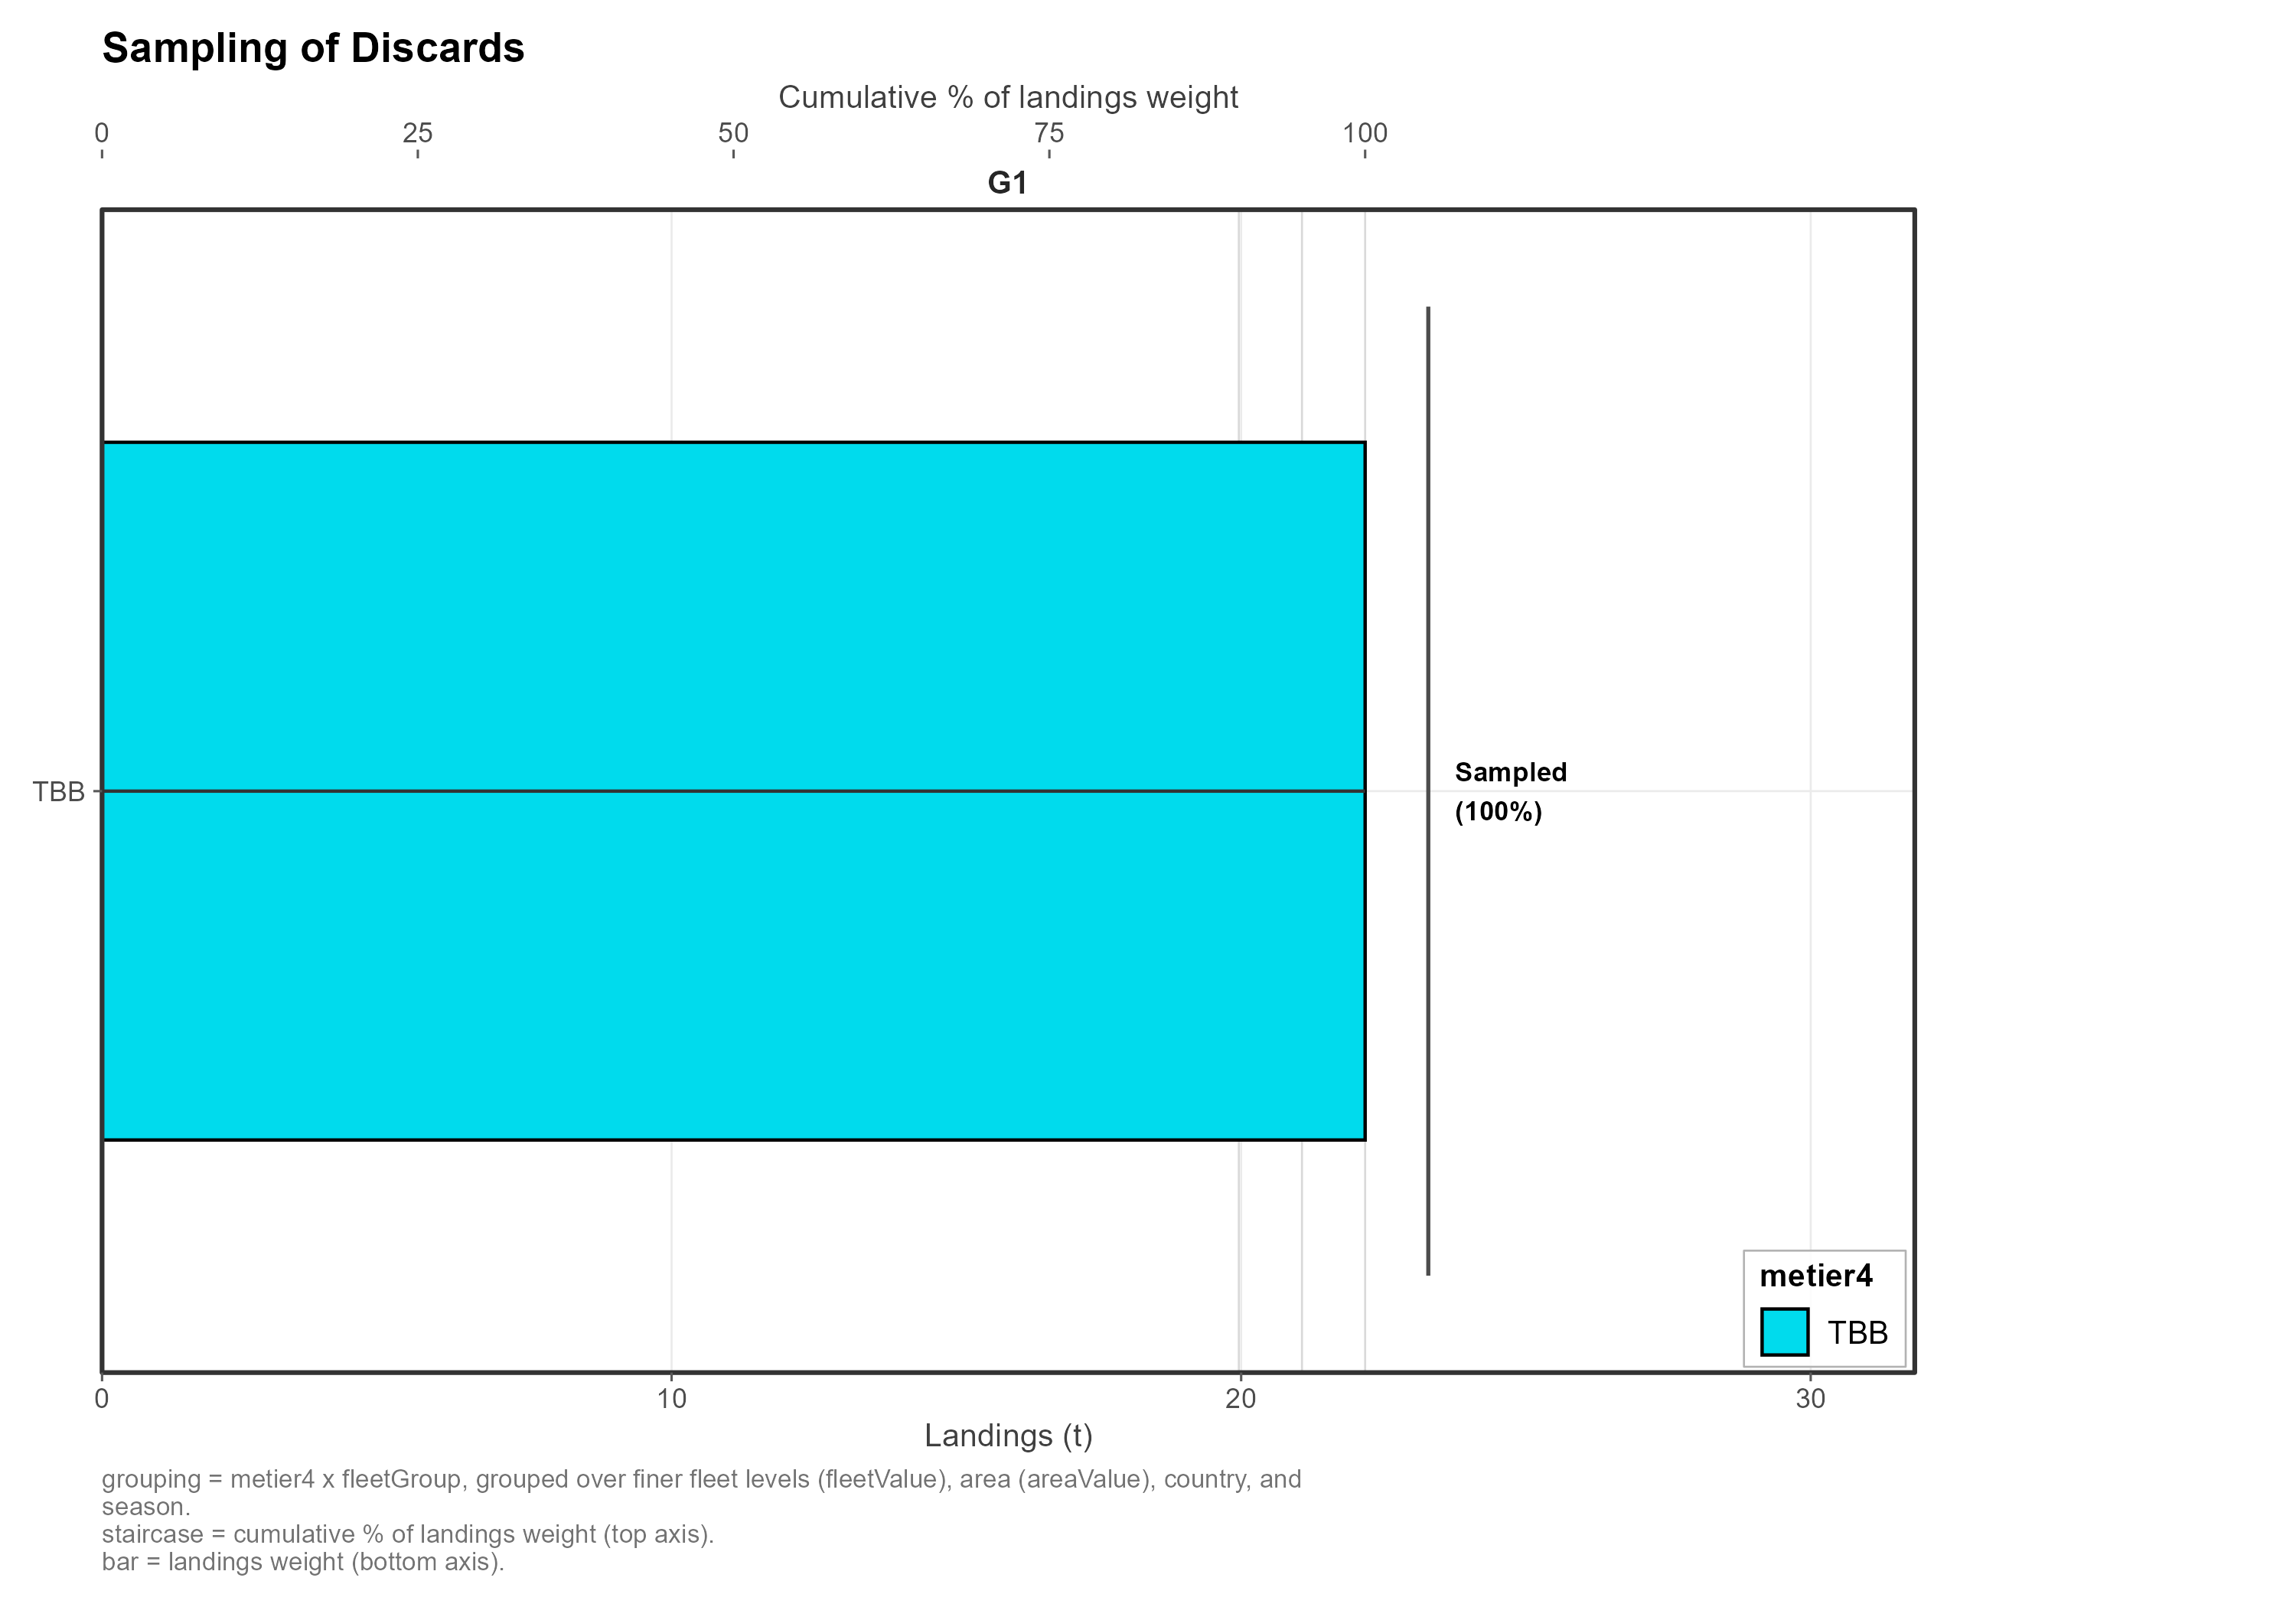
\includegraphics[width=1\linewidth,height=\textheight,keepaspectratio,alt={Three panels for the gillnets, the otter trawls and the rest, with the share of the landings sampled in 27.3.a.21.}]{../../../output/figures/2_discard_raising/discard_raising_14.png}

}

\caption{\label{fig-coverage-3a21}Sampling of the discards in the
Kattegat (27.3.a.21), by fleet group. File
\texttt{discard\_raising\_14.png}.}

\end{figure}%

\emph{(this code is no longer in the script)}

\emph{(this code is no longer in the script)}

\begin{longtable}[]{@{}
  >{\raggedright\arraybackslash}p{(\linewidth - 6\tabcolsep) * \real{0.3000}}
  >{\raggedright\arraybackslash}p{(\linewidth - 6\tabcolsep) * \real{0.2400}}
  >{\raggedright\arraybackslash}p{(\linewidth - 6\tabcolsep) * \real{0.2400}}
  >{\raggedright\arraybackslash}p{(\linewidth - 6\tabcolsep) * \real{0.2200}}@{}}

\caption{\label{tbl-groups-alt}The groups of the alternative that differ
from the usual method; G1, G4 and G5 are the same.}

\tabularnewline

\toprule\noalign{}
\begin{minipage}[b]{\linewidth}\raggedright
Group
\end{minipage} & \begin{minipage}[b]{\linewidth}\raggedright
Raising strata
\end{minipage} & \begin{minipage}[b]{\linewidth}\raggedright
Donors
\end{minipage} & \begin{minipage}[b]{\linewidth}\raggedright
Why
\end{minipage} \\
\midrule\noalign{}
\endhead
\bottomrule\noalign{}
\endlastfoot
G2\_GTR\_GNS & Nets outside 27.3.a.21 & The same strata & The ratio of
the rest of the area. \\
G2b\_GTR\_GNS\_3a21 & Nets in 27.3.a.21 & The same strata (27.3.a.21
only) & A higher ratio, well sampled. \\
G3\_OTB\_SSC\_SDN & Otter trawls and seines outside 27.3.a.21 & The same
strata & The ratio of the rest of the area. \\
G3b\_OTB\_SSC\_SDN\_3a21 & Otter trawls and seines in 27.3.a.21 & The
same strata (27.3.a.21 only) & A higher ratio, well sampled. \\

\end{longtable}

The strata of G2b and G3b are now raised at the level of their own
sampled neighbours in the Kattegat, higher than the rest of their gear
(Figure~\ref{fig-dr-alt}).

\begin{figure}[htbp]

\centering{

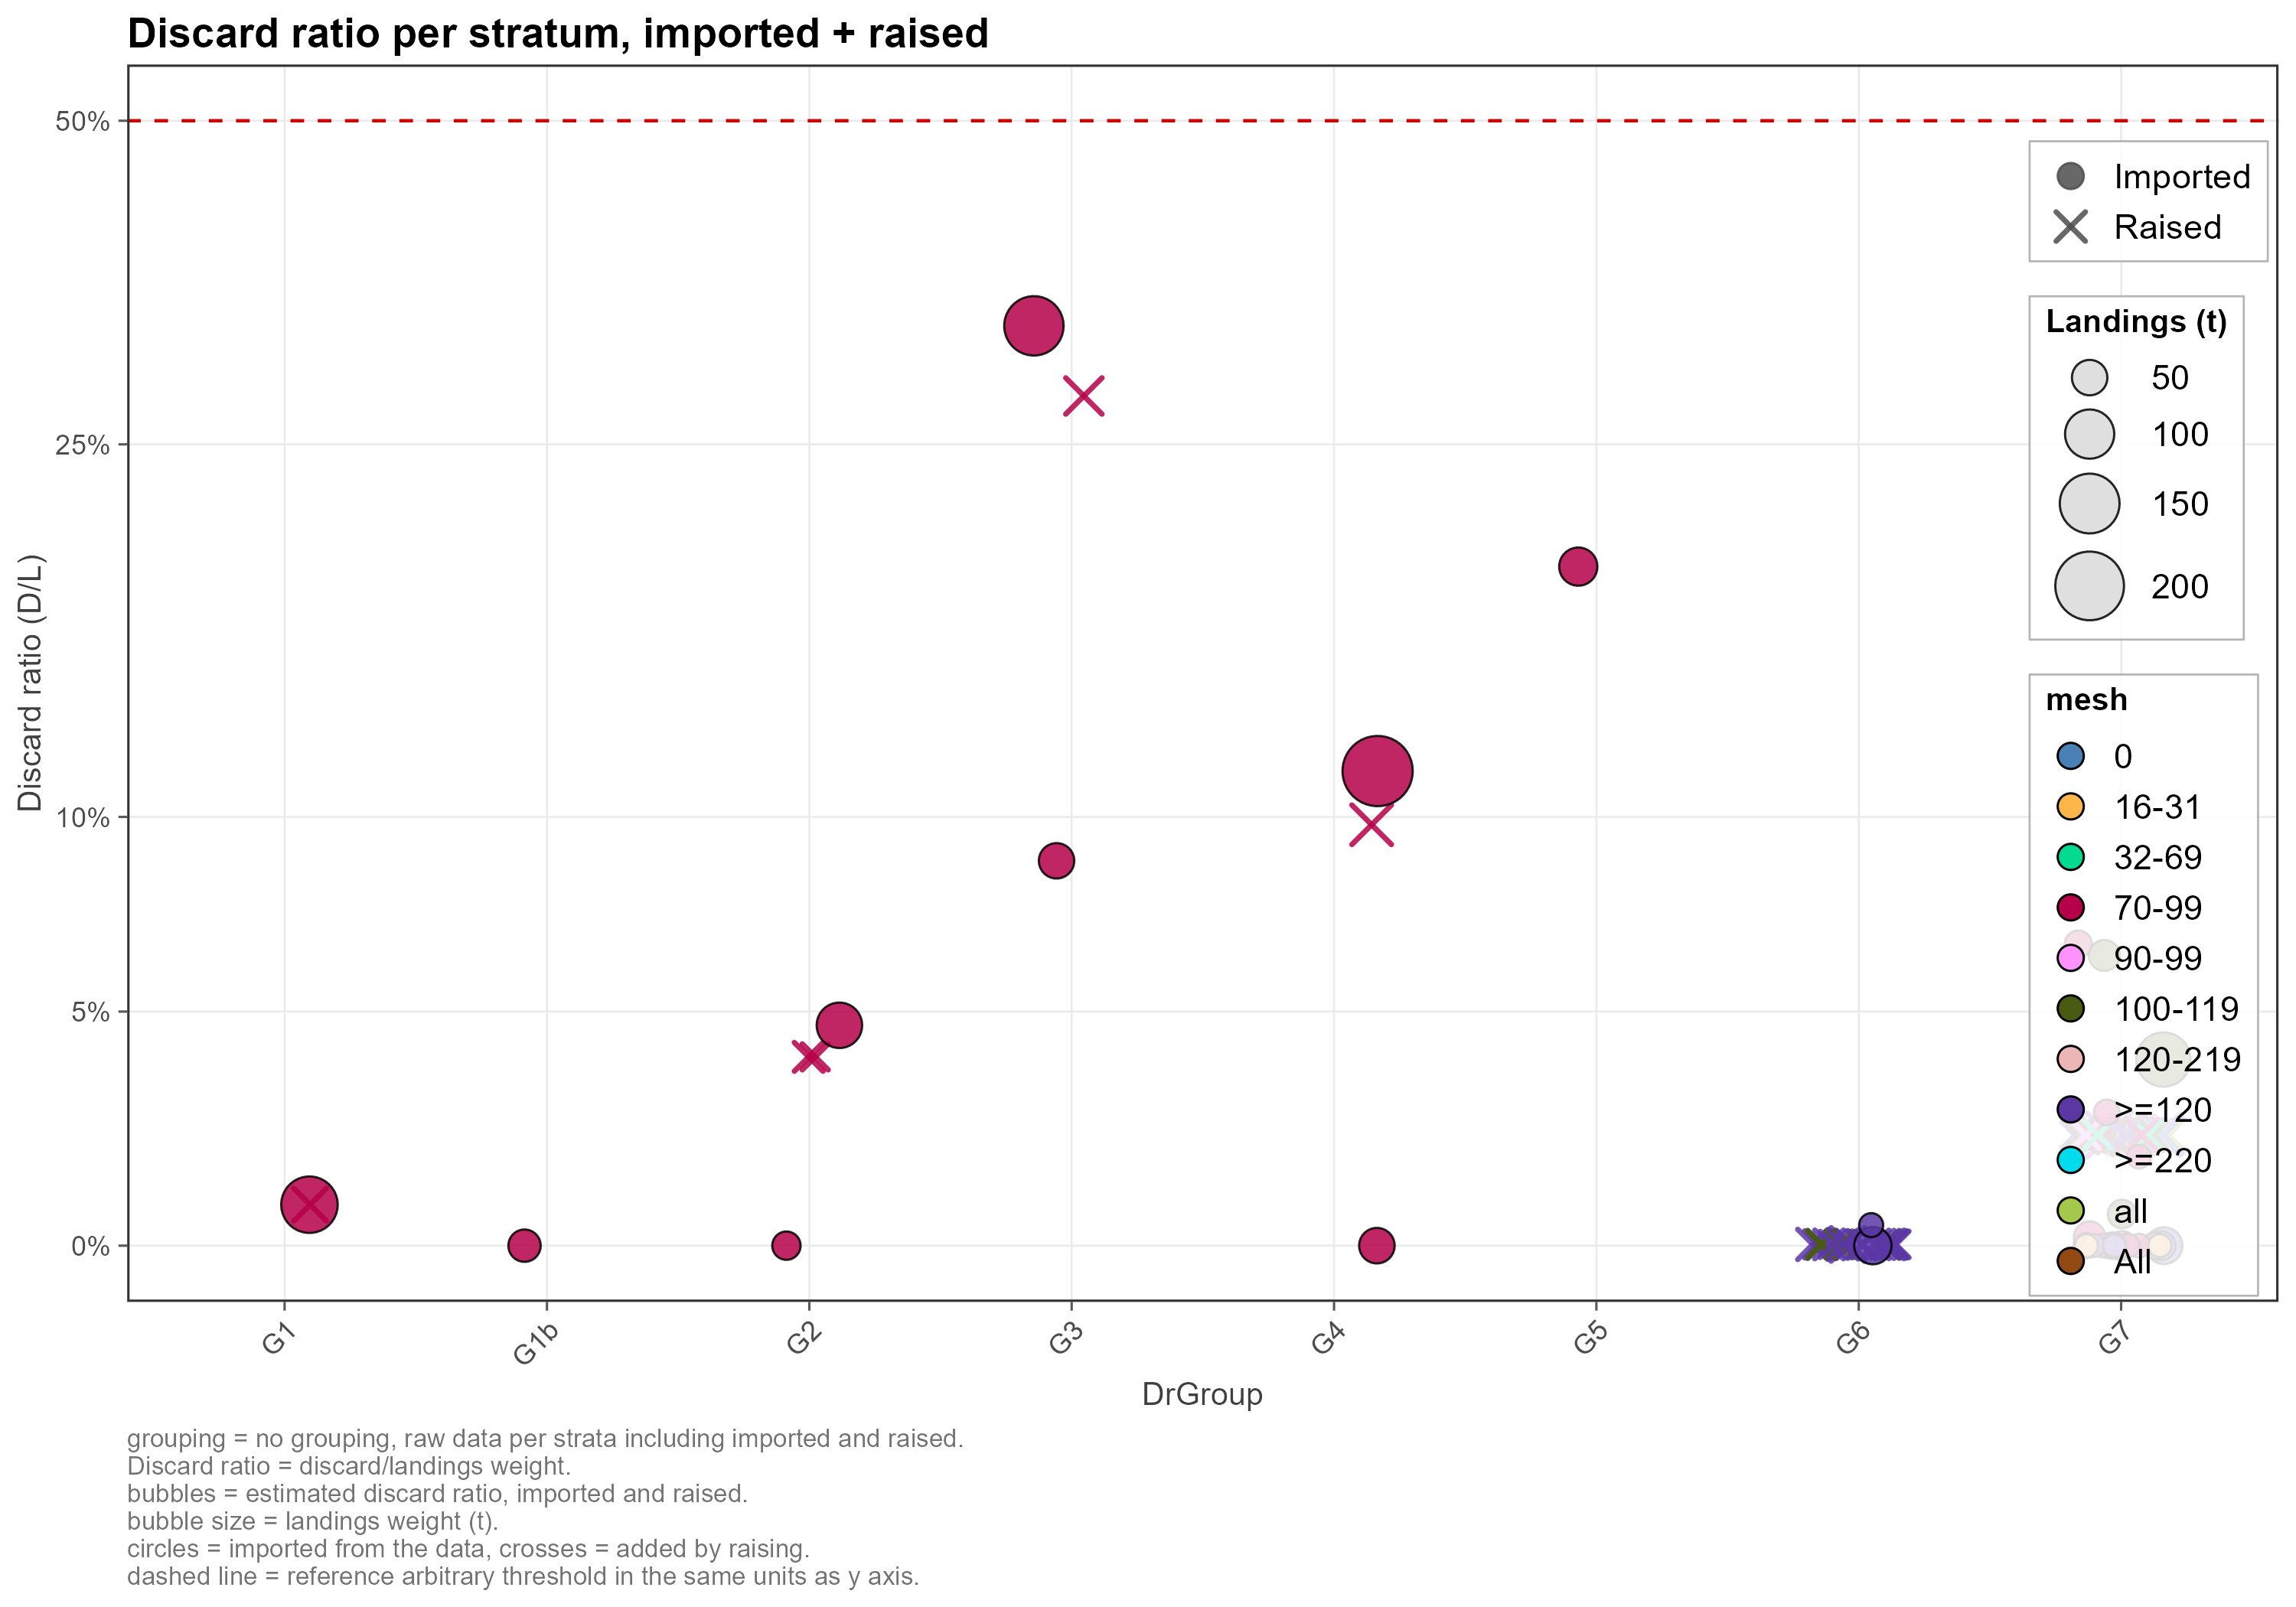
\includegraphics[width=1\linewidth,height=\textheight,keepaspectratio,alt={Points of the discard ratio for each of the six groups, with the raised strata of G2b at a high ratio and those of G3b above the rest of G3.}]{../../../output/figures/2_discard_raising/discard_raising_18.png}

}

\caption{\label{fig-dr-alt}The discard ratio of every stratum after the
alternative raising, by group: circles are imported strata, crosses the
raised ones. File \texttt{discard\_raising\_18.png}.}

\end{figure}%

\subsection{The two methods compared}\label{the-two-methods-compared}

The comparison table of the two methods is saved by
\texttt{model\_discard\_raising.R} in
\texttt{output/raising\_scenarios\_comparison.csv}: run the script to
have it here. The figure below compares the two.

\begin{figure}[htbp]

\centering{

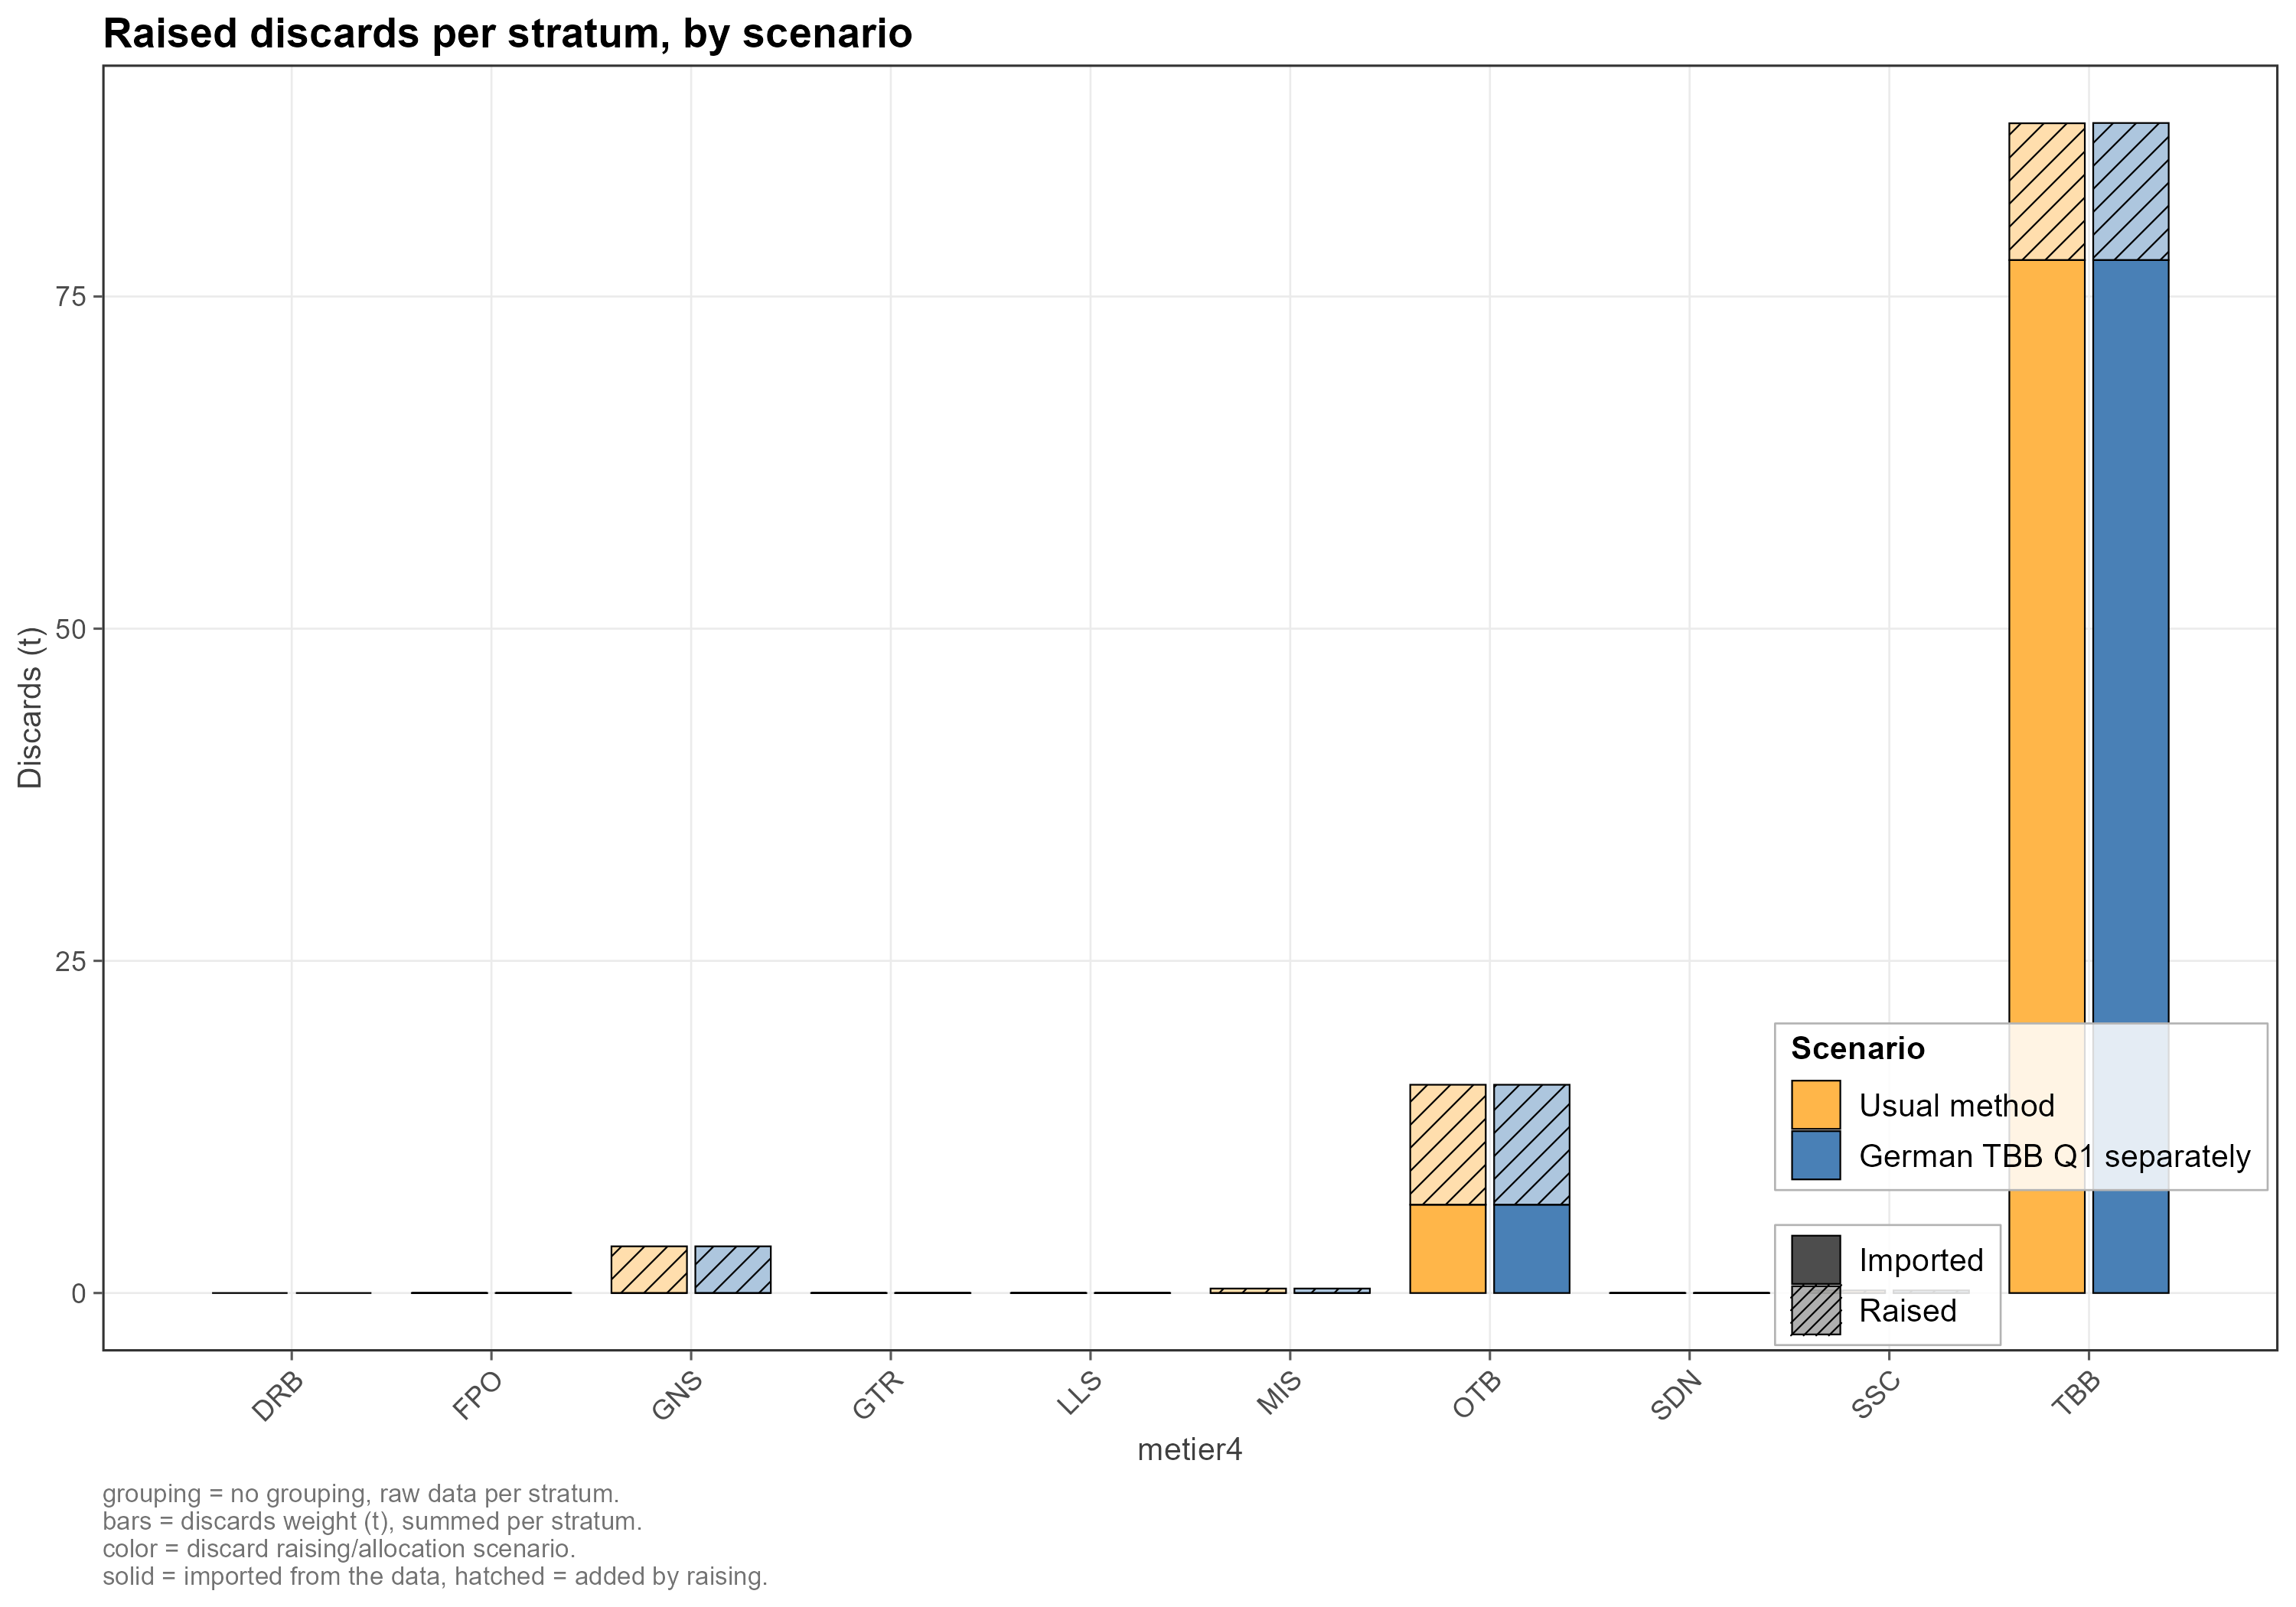
\includegraphics[width=1\linewidth,height=\textheight,keepaspectratio,alt={Pairs of bars for each metier, one for each method, with the imported discards solid and the raised discards hatched.}]{../../../output/figures/2_discard_raising/discard_raising_20.png}

}

\caption{\label{fig-compare}The discards raised and imported by metier,
for the two methods: colour is the method, solid is imported and hatched
is raised. File \texttt{discard\_raising\_20.png}.}

\end{figure}%

The CC and the DC below are made from the usual method: it is the
raising that \texttt{model\_discard\_raising.R} saves in
\texttt{model/catch\_data\_raised.csv}, which the aggregation reads. The
alternative is kept as a comparison.

\section{age allocation}\label{age-allocation}

\subsection{How the allocation works}\label{how-the-allocation-works}

After the raising every stratum has a catch weight, but a age
distribution only if somebody measured fish in it: there are 0 age
distributions, with 0 fish measured in all. The \textbf{allocation}
gives every stratum one. A stratum that has a sampled distribution keeps
it. One that has none gets one estimated from its group: the numbers at
age of the pooled donors, scaled by the weight of the stratum's catch
over the weight of the catch that was sampled, and the mean weight at
age of the donors, averaged with the numbers at that age as weights. The
estimated distributions are marked as such
(\texttt{sampledOrEstimated}).

The allocation works with \textbf{groups} as the raising does: the
\emph{allocation strata}, which are allocated together and must not
overlap, and the \emph{matched data}, the sampled distributions the
group takes its shape from, which can be a wider pool.
\texttt{check\_group\_conditions()} checks the groups before anything is
allocated. The discards are smaller fish than the landings and have
their own age distributions, so landings and discards are allocated in
groups apart.

\subsection{Where are the age samples?}\label{where-are-the-age-samples}

Most of the landings of the beam trawls and about half of those of the
nets have a age distribution, against a third of the otter trawls and
almost nothing for the rest (Figure~\ref{fig-len-lan}). For the discards
only the beam trawls are well sampled (Figure~\ref{fig-len-dis}). The
thresholds of Figure~\ref{fig-len-heat}, at least half of the landings
covered and at least 100 fish measured, are cleared by the beam trawls
with a mesh of 70-99 mm and by the nets of 220 mm and over, so those two
groups can be allocated on their own samples.

\begin{figure}[htbp]

\centering{

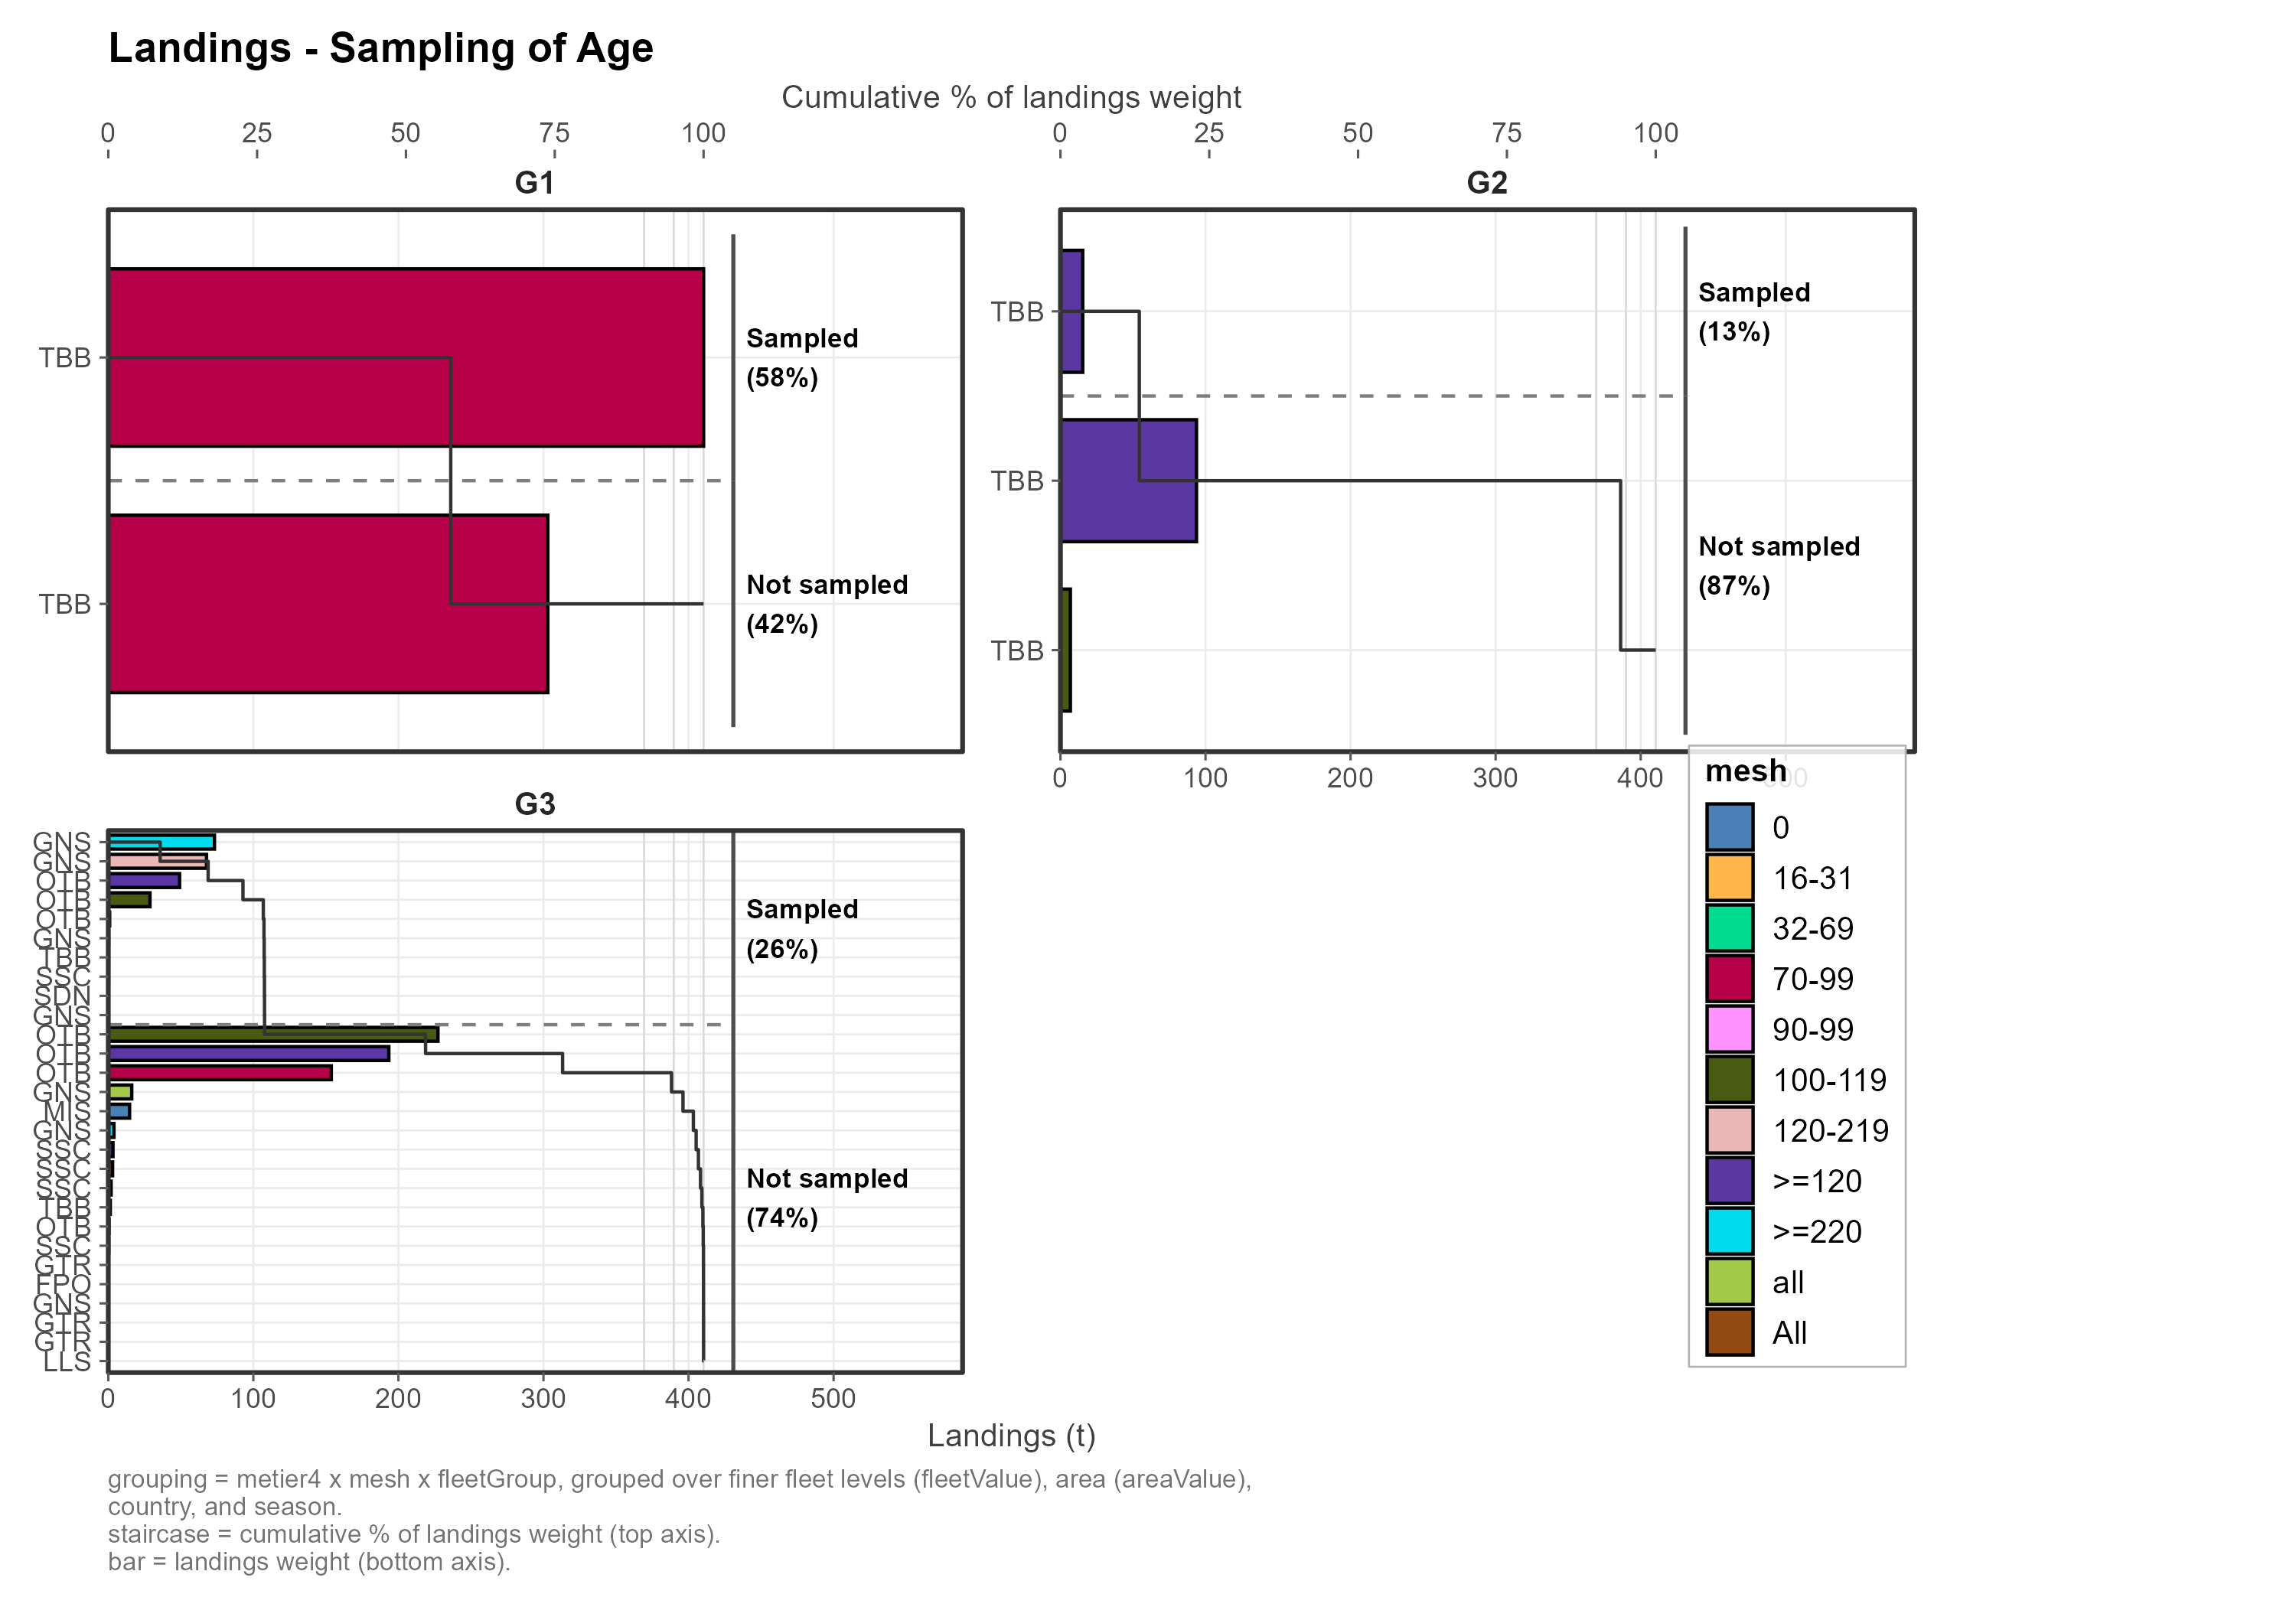
\includegraphics[width=1\linewidth,height=\textheight,keepaspectratio,alt={Four panels, one for each fleet group, of bars of landings by metier and mesh with the share sampled and not sampled.}]{../../../output/figures/3_age_allocation/age_allocation_02.png}

}

\caption{\label{fig-len-lan}Sampling of age in the landings, by fleet
group: the landings by metier and mesh (bars) and the cumulative share
with a age distribution (staircase). File
\texttt{age\_allocation\_02.png}.}

\end{figure}%

\begin{figure}[htbp]

\centering{

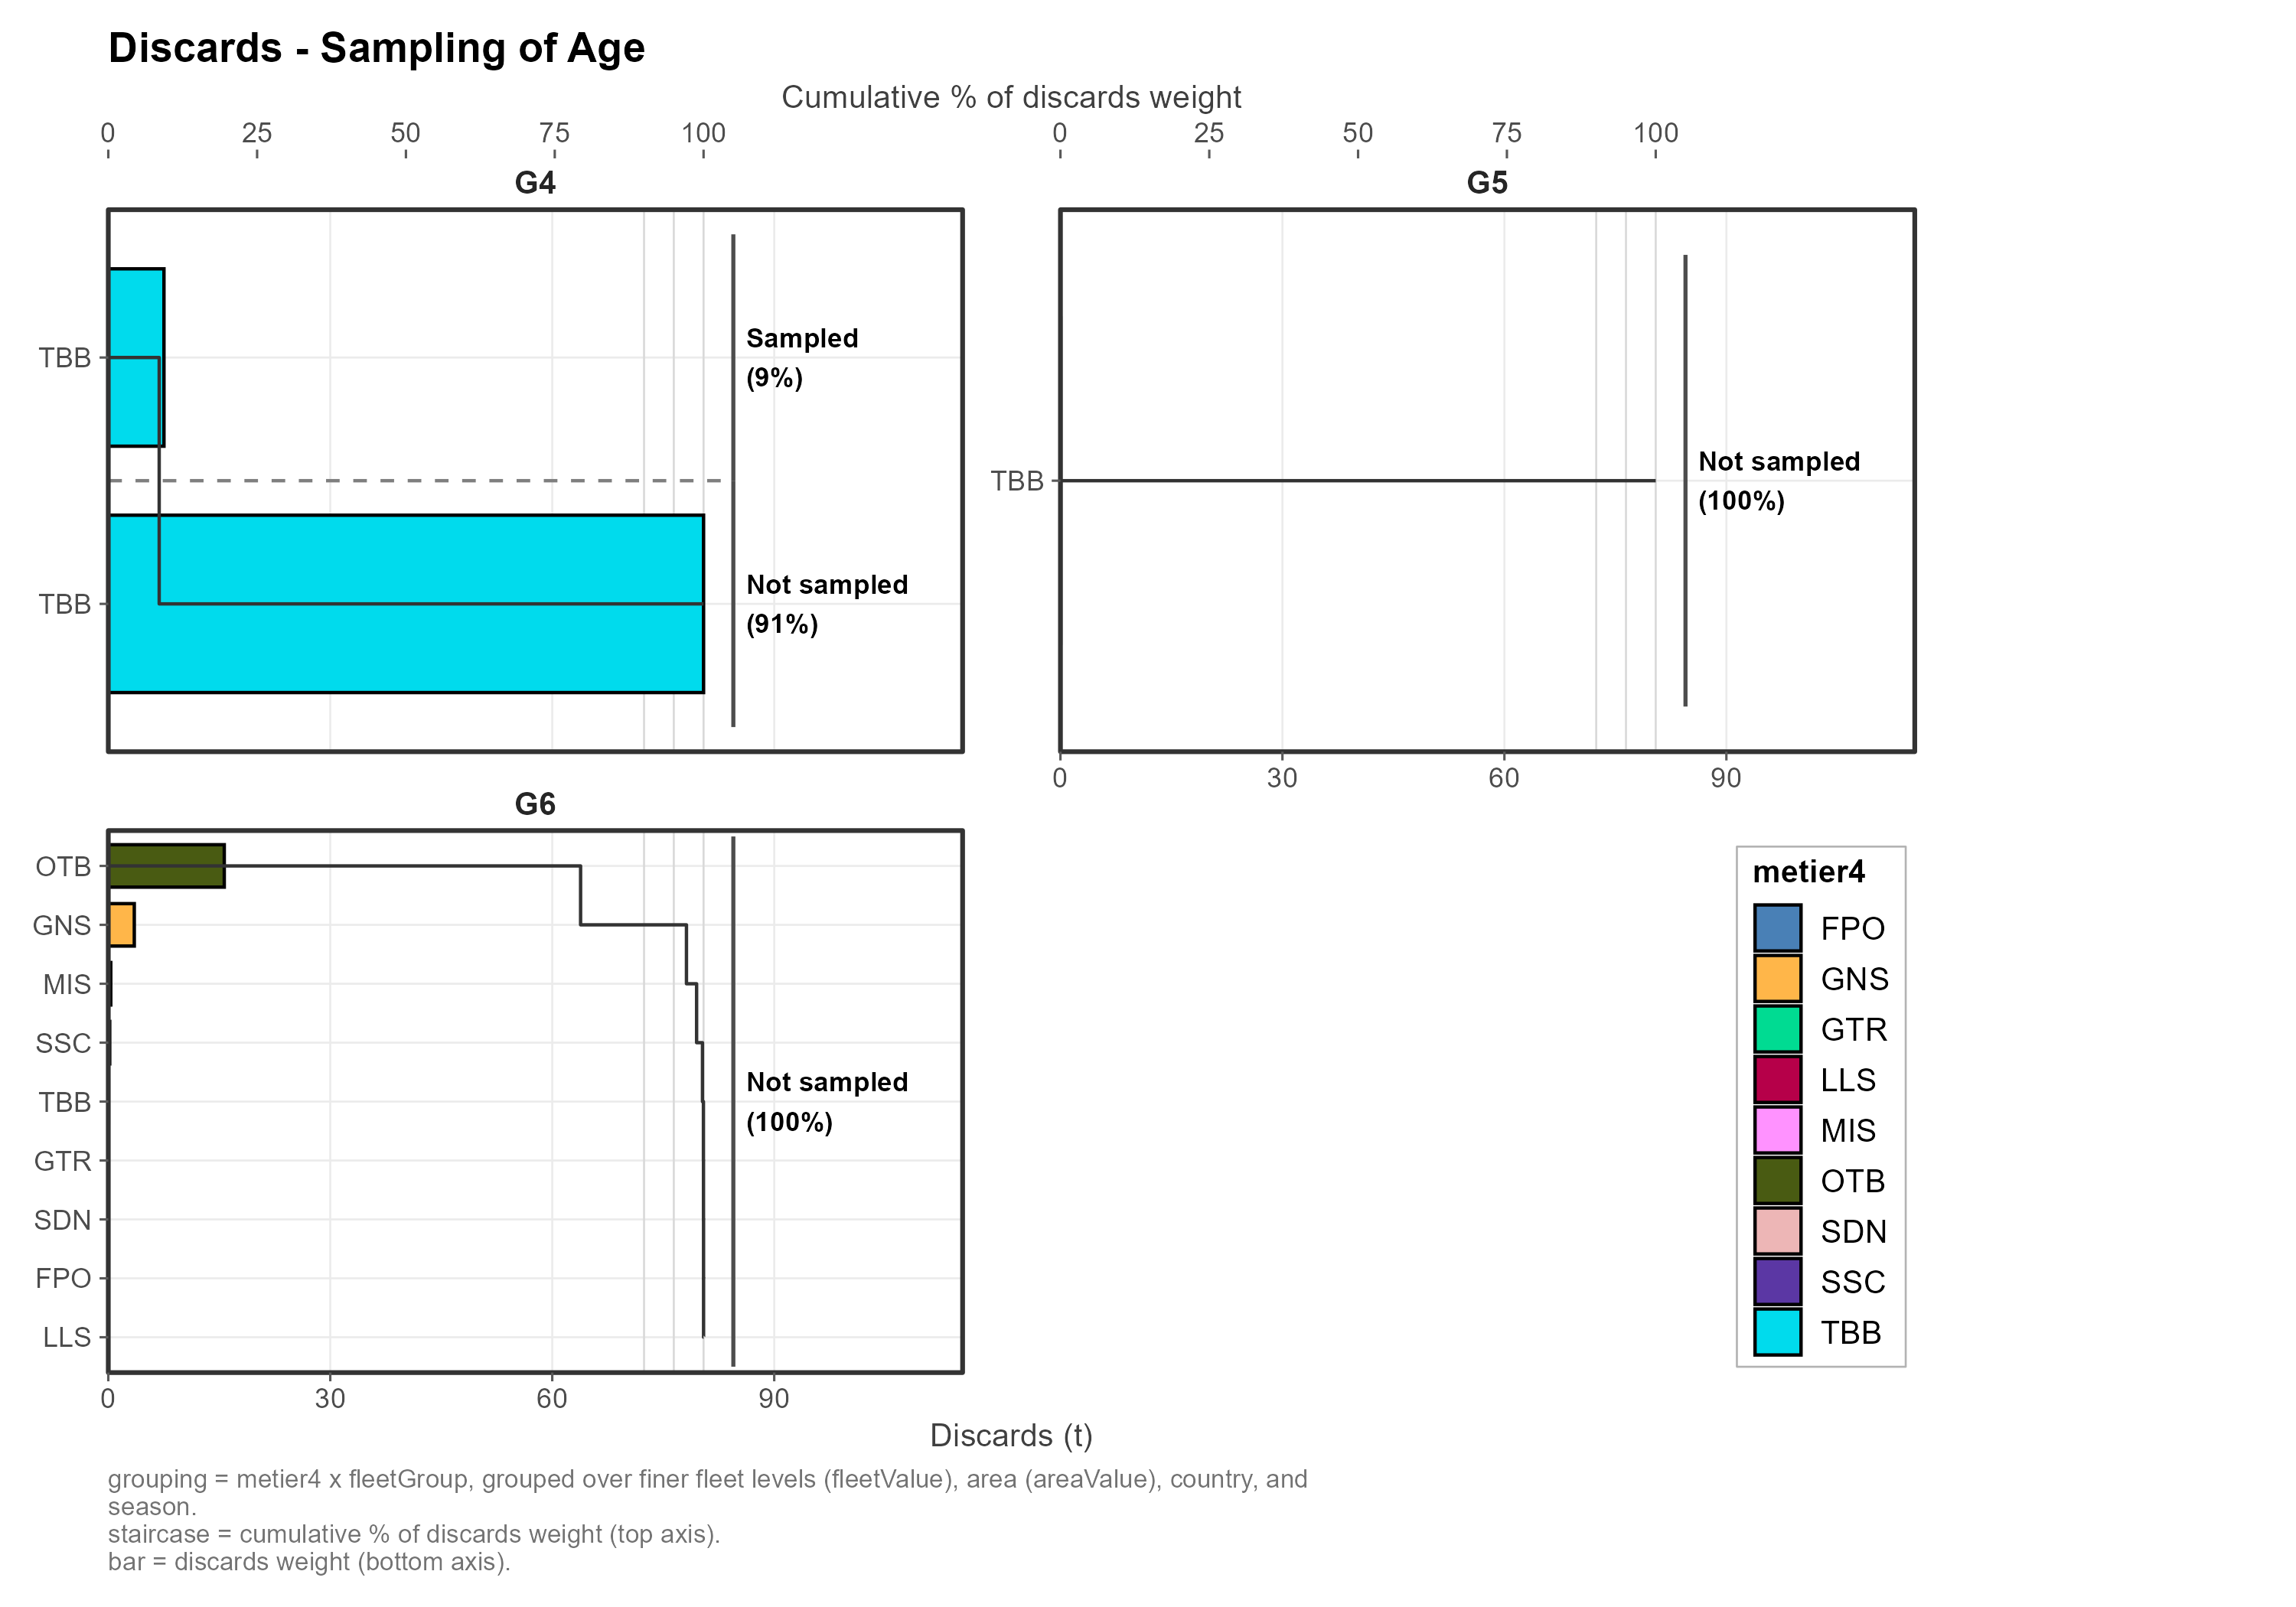
\includegraphics[width=1\linewidth,height=\textheight,keepaspectratio,alt={Four panels, one for each fleet group, of bars of discards by metier with the share sampled and not sampled; the beam trawls are well sampled.}]{../../../output/figures/3_age_allocation/age_allocation_14.png}

}

\caption{\label{fig-len-dis}Sampling of age in the discards, by fleet
group. File \texttt{age\_allocation\_14.png}.}

\end{figure}%

\begin{figure}[htbp]

\centering{

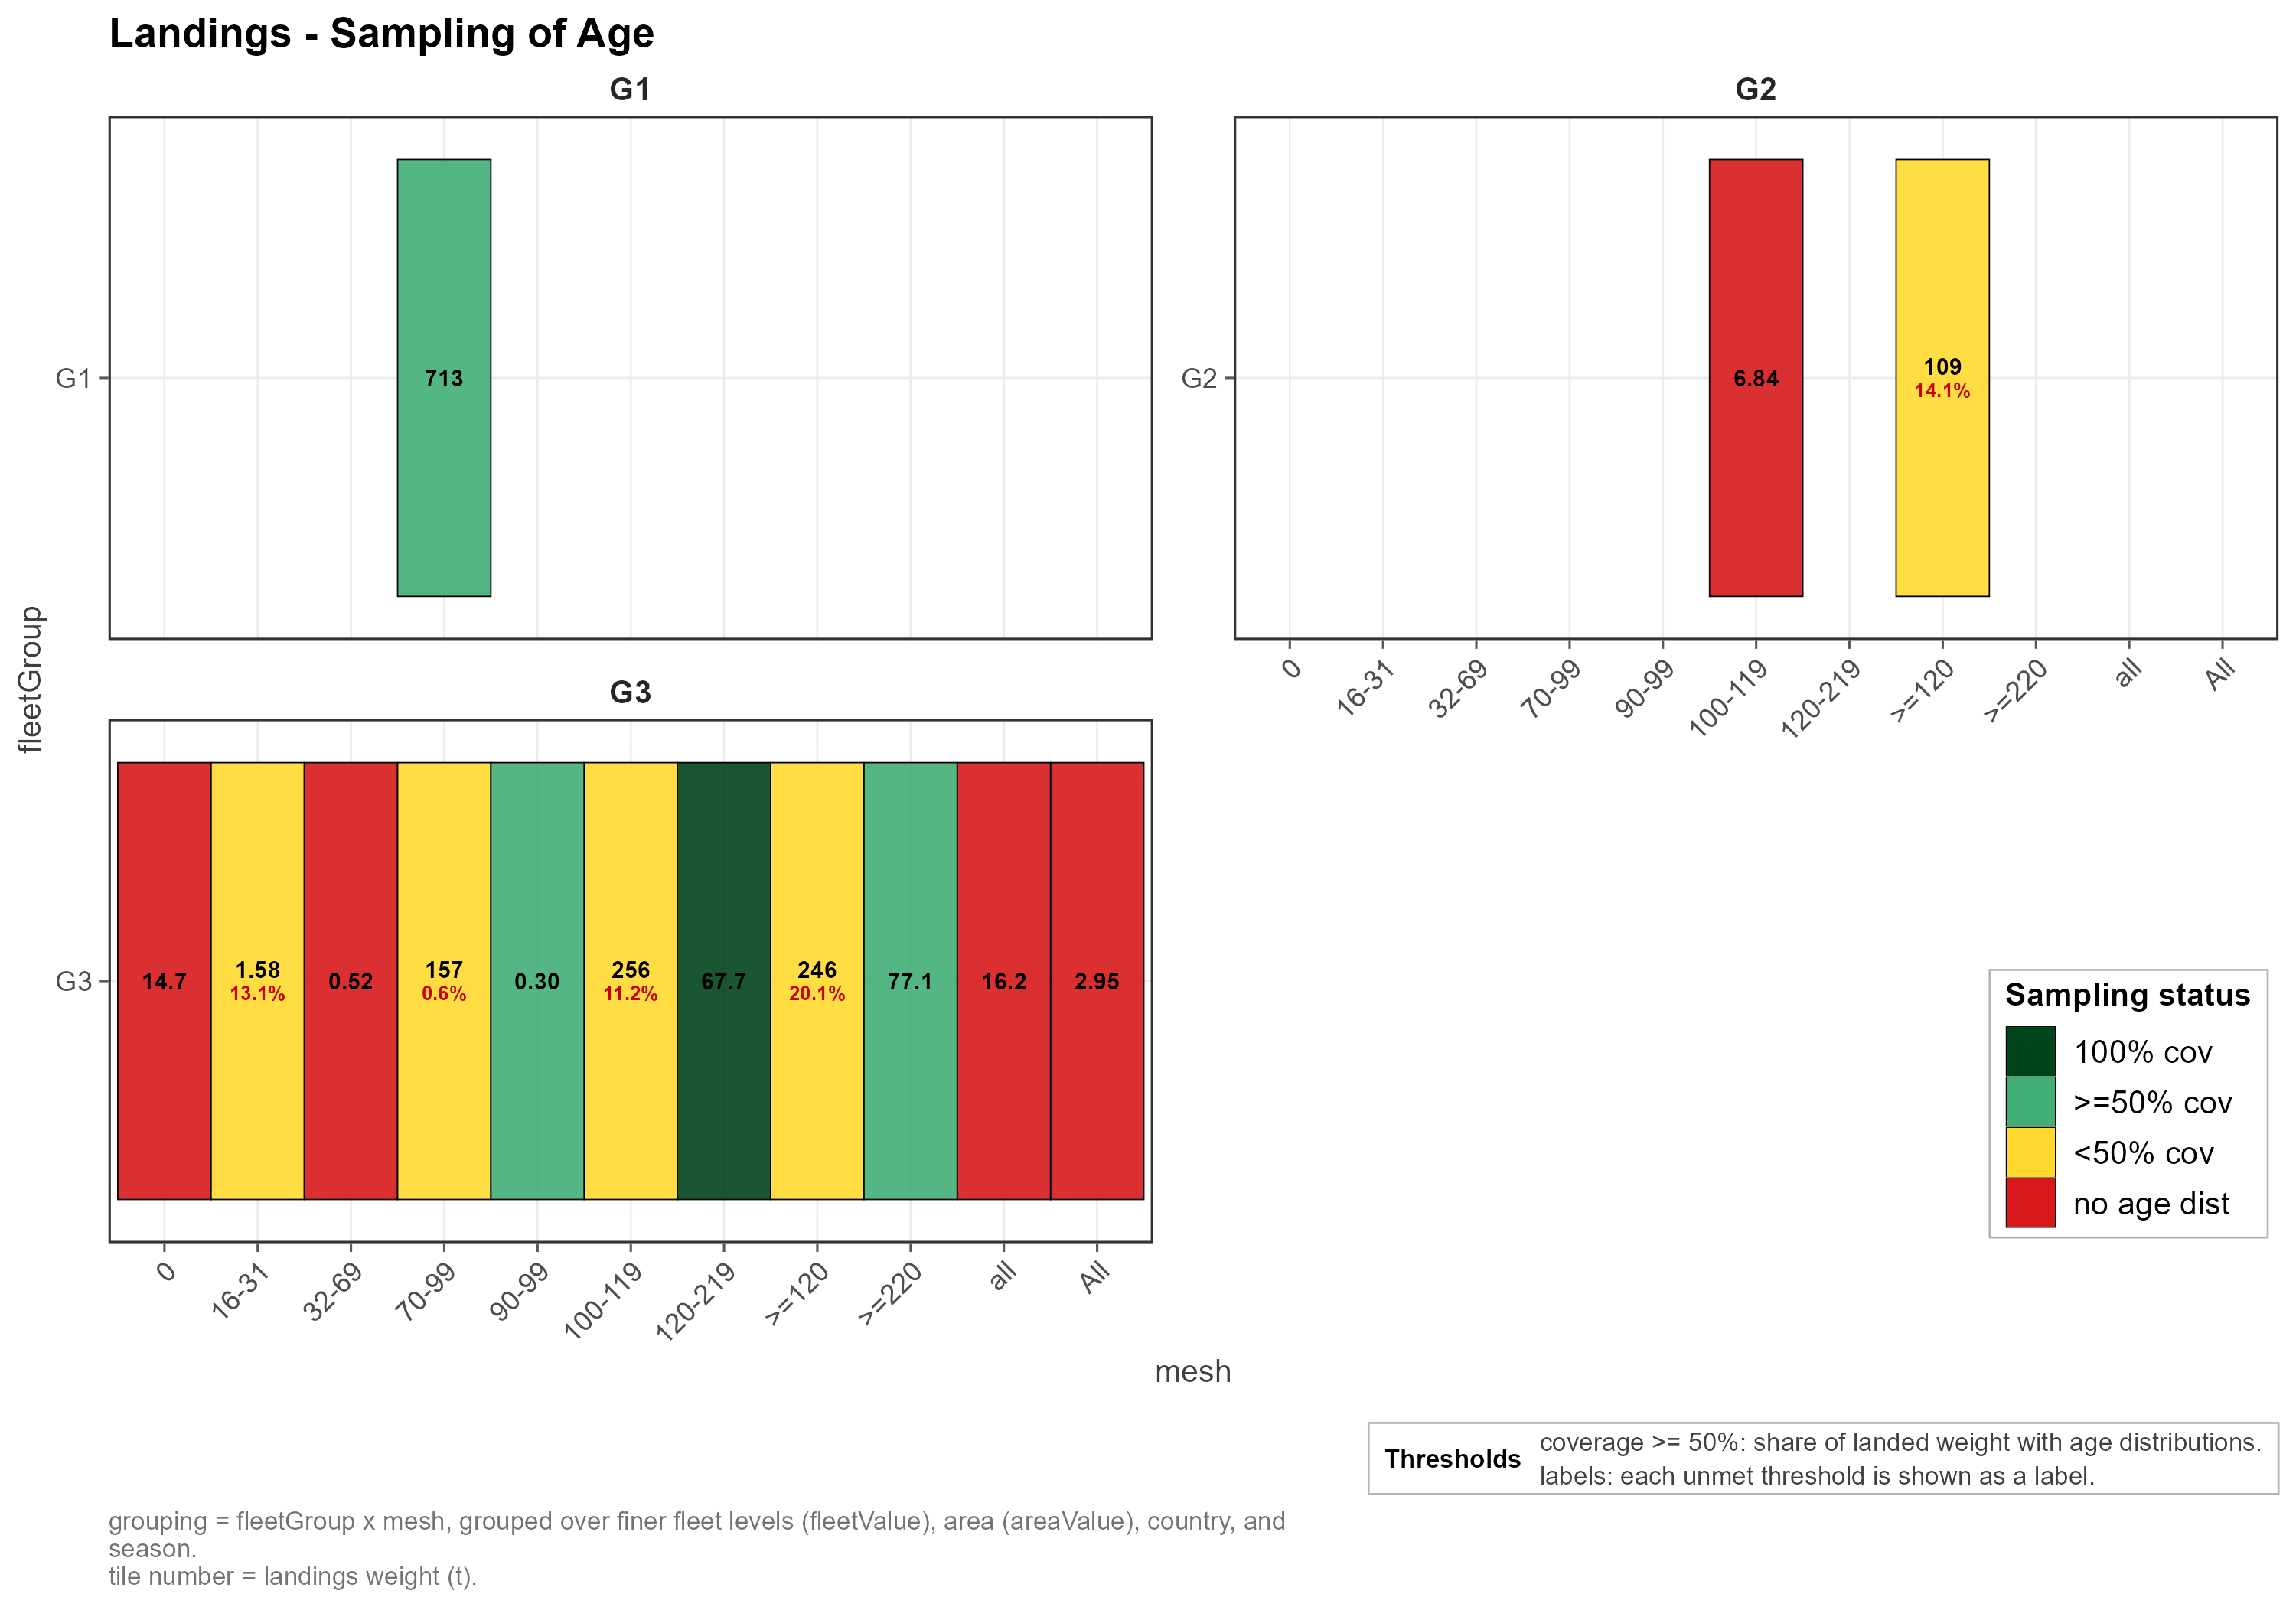
\includegraphics[width=1\linewidth,height=\textheight,keepaspectratio,alt={Four panels of tiles by mesh coloured by whether the coverage and the number of fish measured pass their thresholds, with the landings in tonnes.}]{../../../output/figures/3_age_allocation/age_allocation_04.png}

}

\caption{\label{fig-len-heat}Sampling of age in the landings by fleet
group and mesh against two thresholds: at least 50\% of the landings
with a age distribution and at least 100 fish measured. File
\texttt{age\_allocation\_04.png}.}

\end{figure}%

\subsection{The groups}\label{the-groups}

There are six groups (Table~\ref{tbl-groups-alloc}), written in
\texttt{model\_age\_allocation.R}:

\emph{(this code is no longer in the script)}

\emph{(this code is no longer in the script)}

\begin{longtable}[]{@{}
  >{\raggedright\arraybackslash}p{(\linewidth - 6\tabcolsep) * \real{0.2200}}
  >{\raggedright\arraybackslash}p{(\linewidth - 6\tabcolsep) * \real{0.2600}}
  >{\raggedright\arraybackslash}p{(\linewidth - 6\tabcolsep) * \real{0.2600}}
  >{\raggedright\arraybackslash}p{(\linewidth - 6\tabcolsep) * \real{0.2600}}@{}}

\caption{\label{tbl-groups-alloc}The six allocation groups.}

\tabularnewline

\toprule\noalign{}
\begin{minipage}[b]{\linewidth}\raggedright
Group
\end{minipage} & \begin{minipage}[b]{\linewidth}\raggedright
Allocation strata
\end{minipage} & \begin{minipage}[b]{\linewidth}\raggedright
Donors
\end{minipage} & \begin{minipage}[b]{\linewidth}\raggedright
Why
\end{minipage} \\
\midrule\noalign{}
\endhead
\bottomrule\noalign{}
\endlastfoot
G1\_TBB\_LAN & Landings of the beam trawls & The same strata & Enough
samples (coverage and fish measured) in its main mesh: its own
distribution. \\
G2\_GTR\_GNS\_LAN & Landings of the nets & The same strata & Enough
samples in its main mesh: its own distribution. \\
G3\_REST\_LAN & Landings of the other metiers & All the landings & Too
little sampled: it draws on all the landings. \\
G4\_TBB\_DIS & Discards of the beam trawls & The same strata & Well
sampled: its own distribution. \\
G5\_REST\_DIS & The other discards and the BMS & All the discards and
the BMS, beam trawls included & Too little sampled: it draws on all the
discards. \\
G6\_IBC & The incidental bycatch fleet, all catch categories & All the
samples & No catch: nothing to allocate. \\

\end{longtable}

\subsection{What the allocation did}\label{what-the-allocation-did}

Every catch row got a distribution (none is left without one): 46
distributions are sampled and 252 were estimated. By weight, 39\% of the
landings and 9\% of the discards have a sampled distribution; the rest
takes the shape of its donors (Table~\ref{tbl-alloc-result}).

\begin{longtable}[]{@{}
  >{\raggedright\arraybackslash}p{(\linewidth - 12\tabcolsep) * \real{0.2100}}
  >{\raggedleft\arraybackslash}p{(\linewidth - 12\tabcolsep) * \real{0.0900}}
  >{\raggedleft\arraybackslash}p{(\linewidth - 12\tabcolsep) * \real{0.1300}}
  >{\raggedleft\arraybackslash}p{(\linewidth - 12\tabcolsep) * \real{0.1300}}
  >{\raggedleft\arraybackslash}p{(\linewidth - 12\tabcolsep) * \real{0.1700}}
  >{\raggedleft\arraybackslash}p{(\linewidth - 12\tabcolsep) * \real{0.1700}}
  >{\raggedleft\arraybackslash}p{(\linewidth - 12\tabcolsep) * \real{0.1000}}@{}}

\caption{\label{tbl-alloc-result}The allocation by group: the
distributions that are sampled or estimated, and the catch (tonnes) they
belong to.}

\tabularnewline

\toprule\noalign{}
\begin{minipage}[b]{\linewidth}\raggedright
Group
\end{minipage} & \begin{minipage}[b]{\linewidth}\raggedleft
Catch rows
\end{minipage} & \begin{minipage}[b]{\linewidth}\raggedleft
Sampled distributions
\end{minipage} & \begin{minipage}[b]{\linewidth}\raggedleft
Estimated distributions
\end{minipage} & \begin{minipage}[b]{\linewidth}\raggedleft
Catch with a sampled distribution (t)
\end{minipage} & \begin{minipage}[b]{\linewidth}\raggedleft
Catch with an estimated distribution (t)
\end{minipage} & \begin{minipage}[b]{\linewidth}\raggedleft
Sampled (\%)
\end{minipage} \\
\midrule\noalign{}
\endhead
\bottomrule\noalign{}
\endlastfoot
G1 & 14 & 4 & 10 & 410.4 & 303.0 & 58 \\
G2 & 26 & 5 & 21 & 15.4 & 100.6 & 13 \\
G3 & 244 & 36 & 208 & 220.6 & 619.6 & 26 \\
G4 & 14 & 1 & 13 & 7.5 & 80.5 & 9 \\
Total & 298 & 46 & 252 & 653.8 & 1,103.7 & 37 \\

\end{longtable}

The numbers at age of the landings show the groups: the beam trawls land
fish of 30 to 40 cm, the nets fish around 50 cm, and the other gears a
broad range; where no samples were taken the distribution is estimated
(hatched) from the donors and scaled to the landings of the stratum
(Figure~\ref{fig-nal-lan}). The discards are smaller fish, and only the
beam trawls have sampled distributions of their own
(Figure~\ref{fig-nal-dis}).

\begin{figure}[htbp]

\centering{

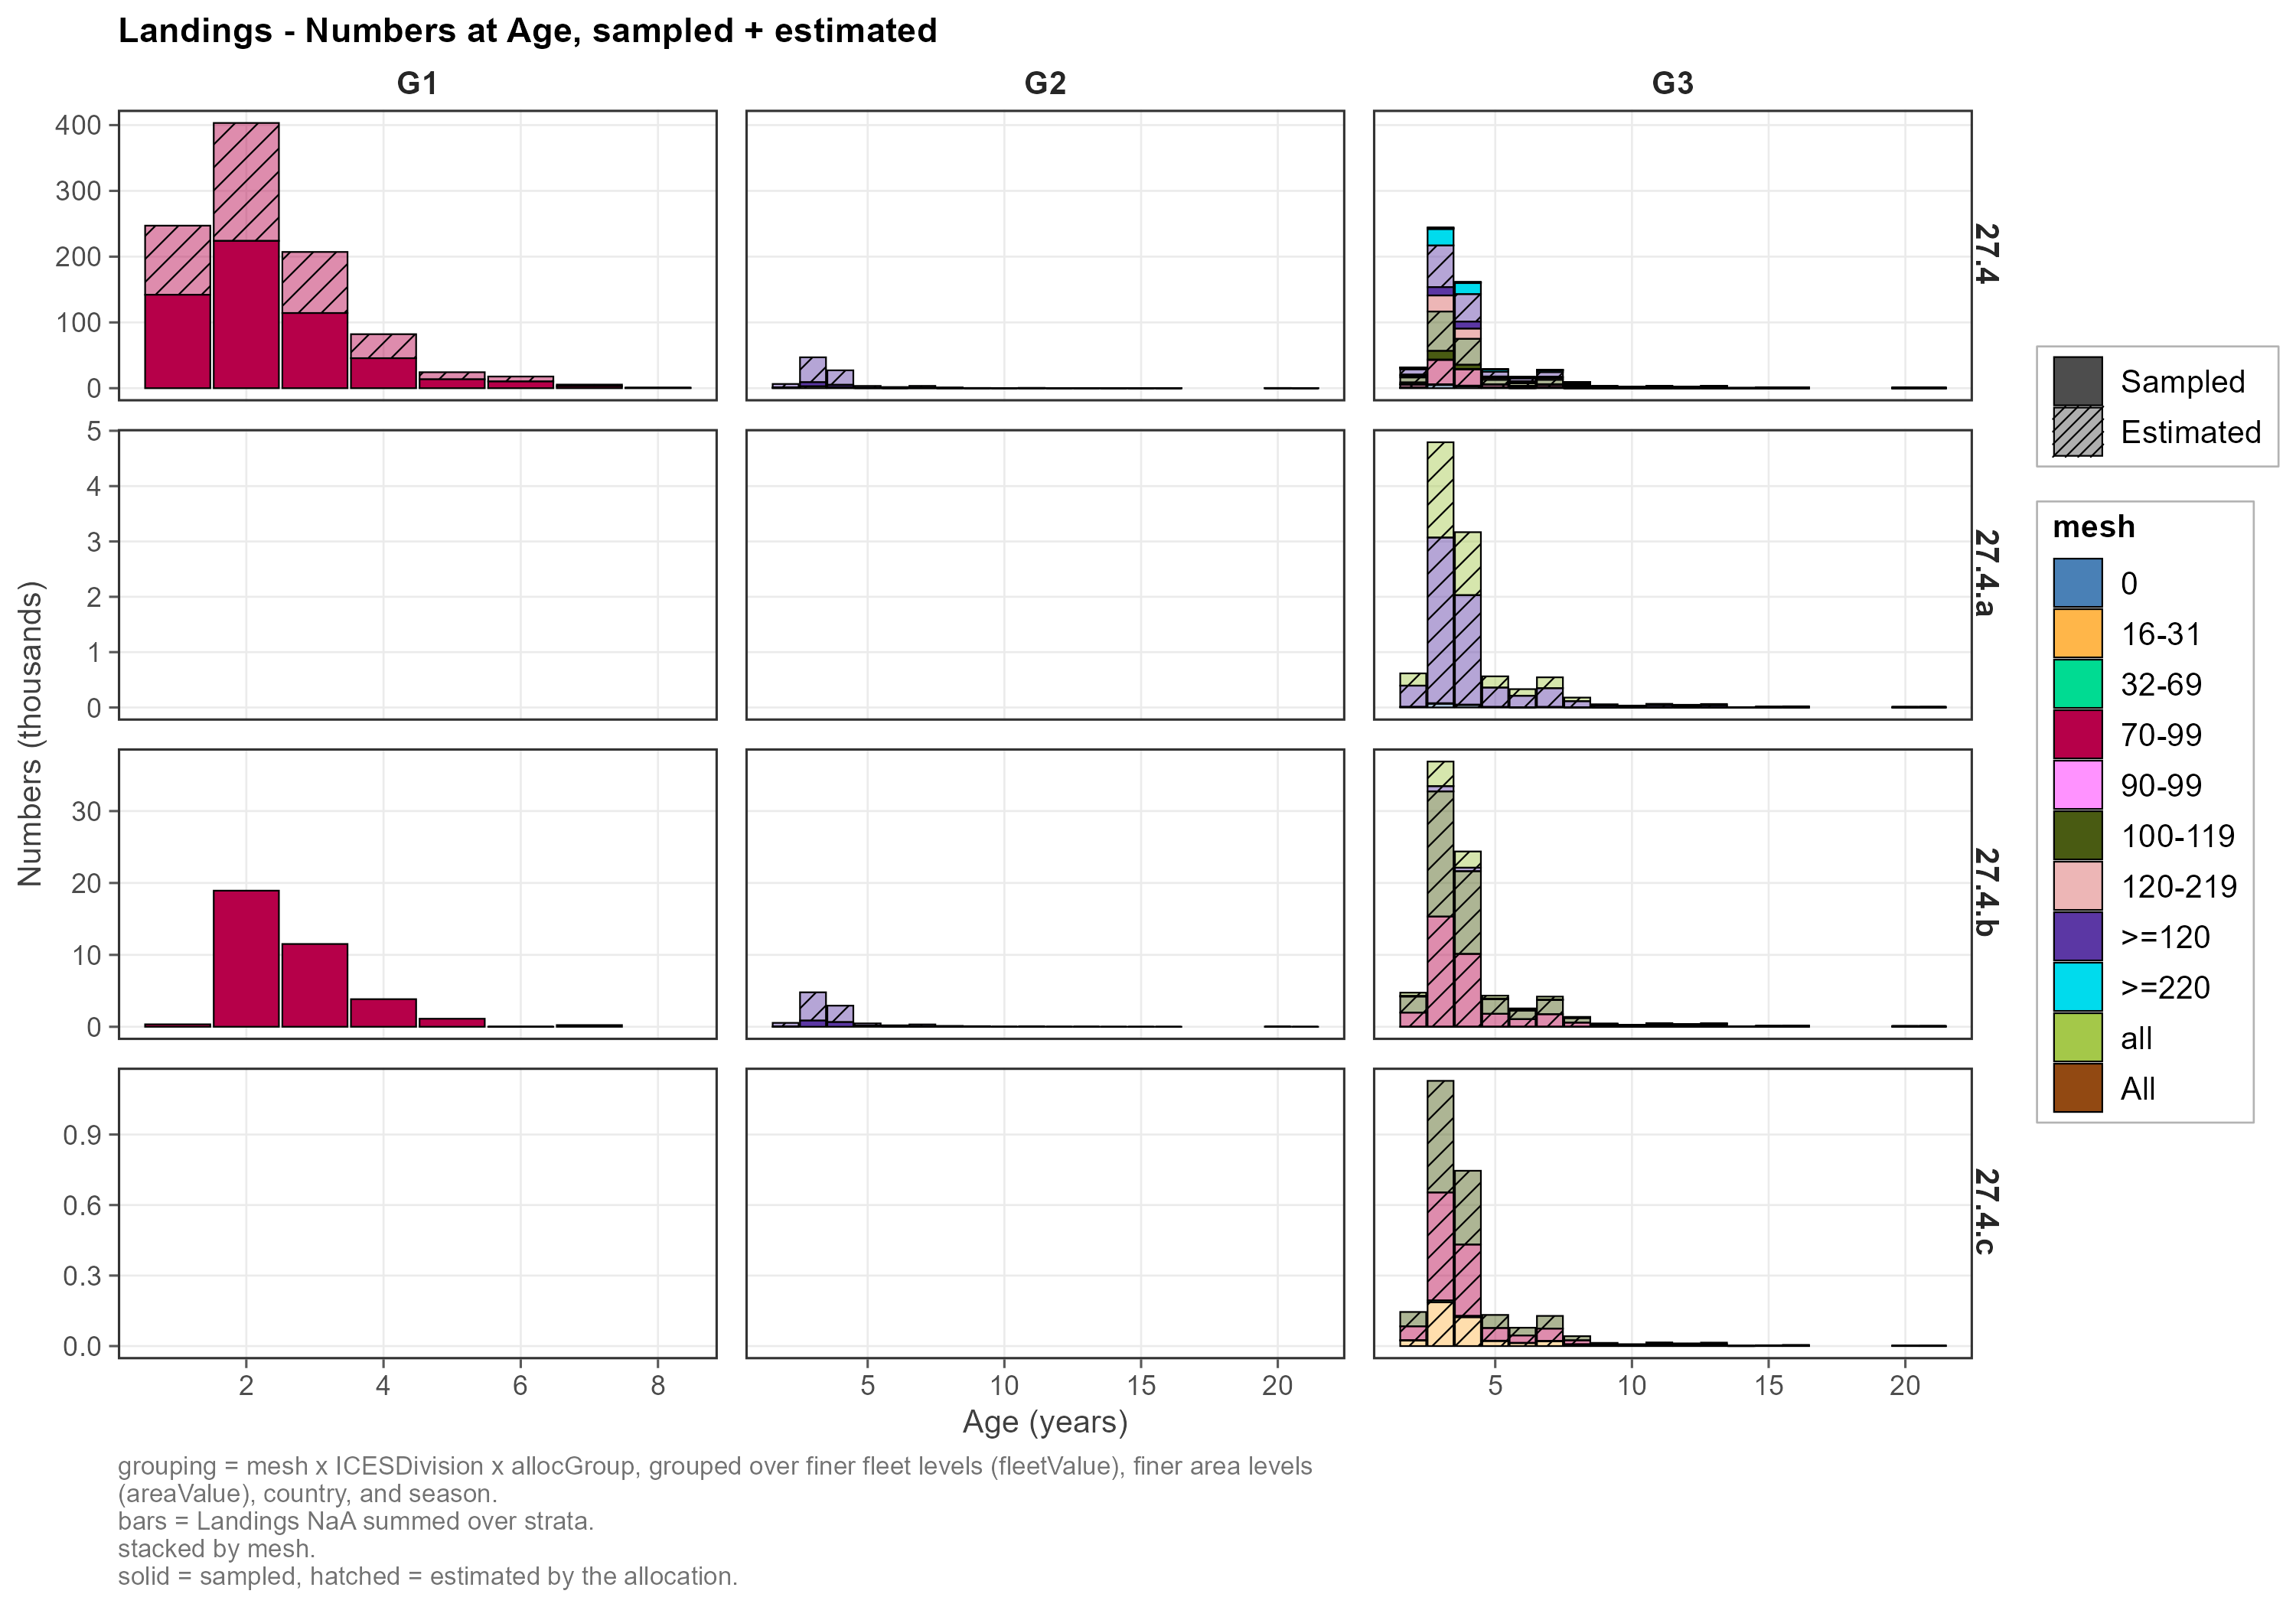
\includegraphics[width=1\linewidth,height=\textheight,keepaspectratio,alt={A grid of histograms of the numbers at age with the allocation groups in columns and the ICES divisions in rows.}]{../../../output/figures/3_age_allocation/age_allocation_19.png}

}

\caption{\label{fig-nal-lan}Numbers at age of the landings, by ICES
division (rows) and allocation group (columns), filled by mesh: solid is
sampled, hatched is estimated by the allocation. File
\texttt{age\_allocation\_22.png}.}

\end{figure}%

\begin{figure}[htbp]

\centering{

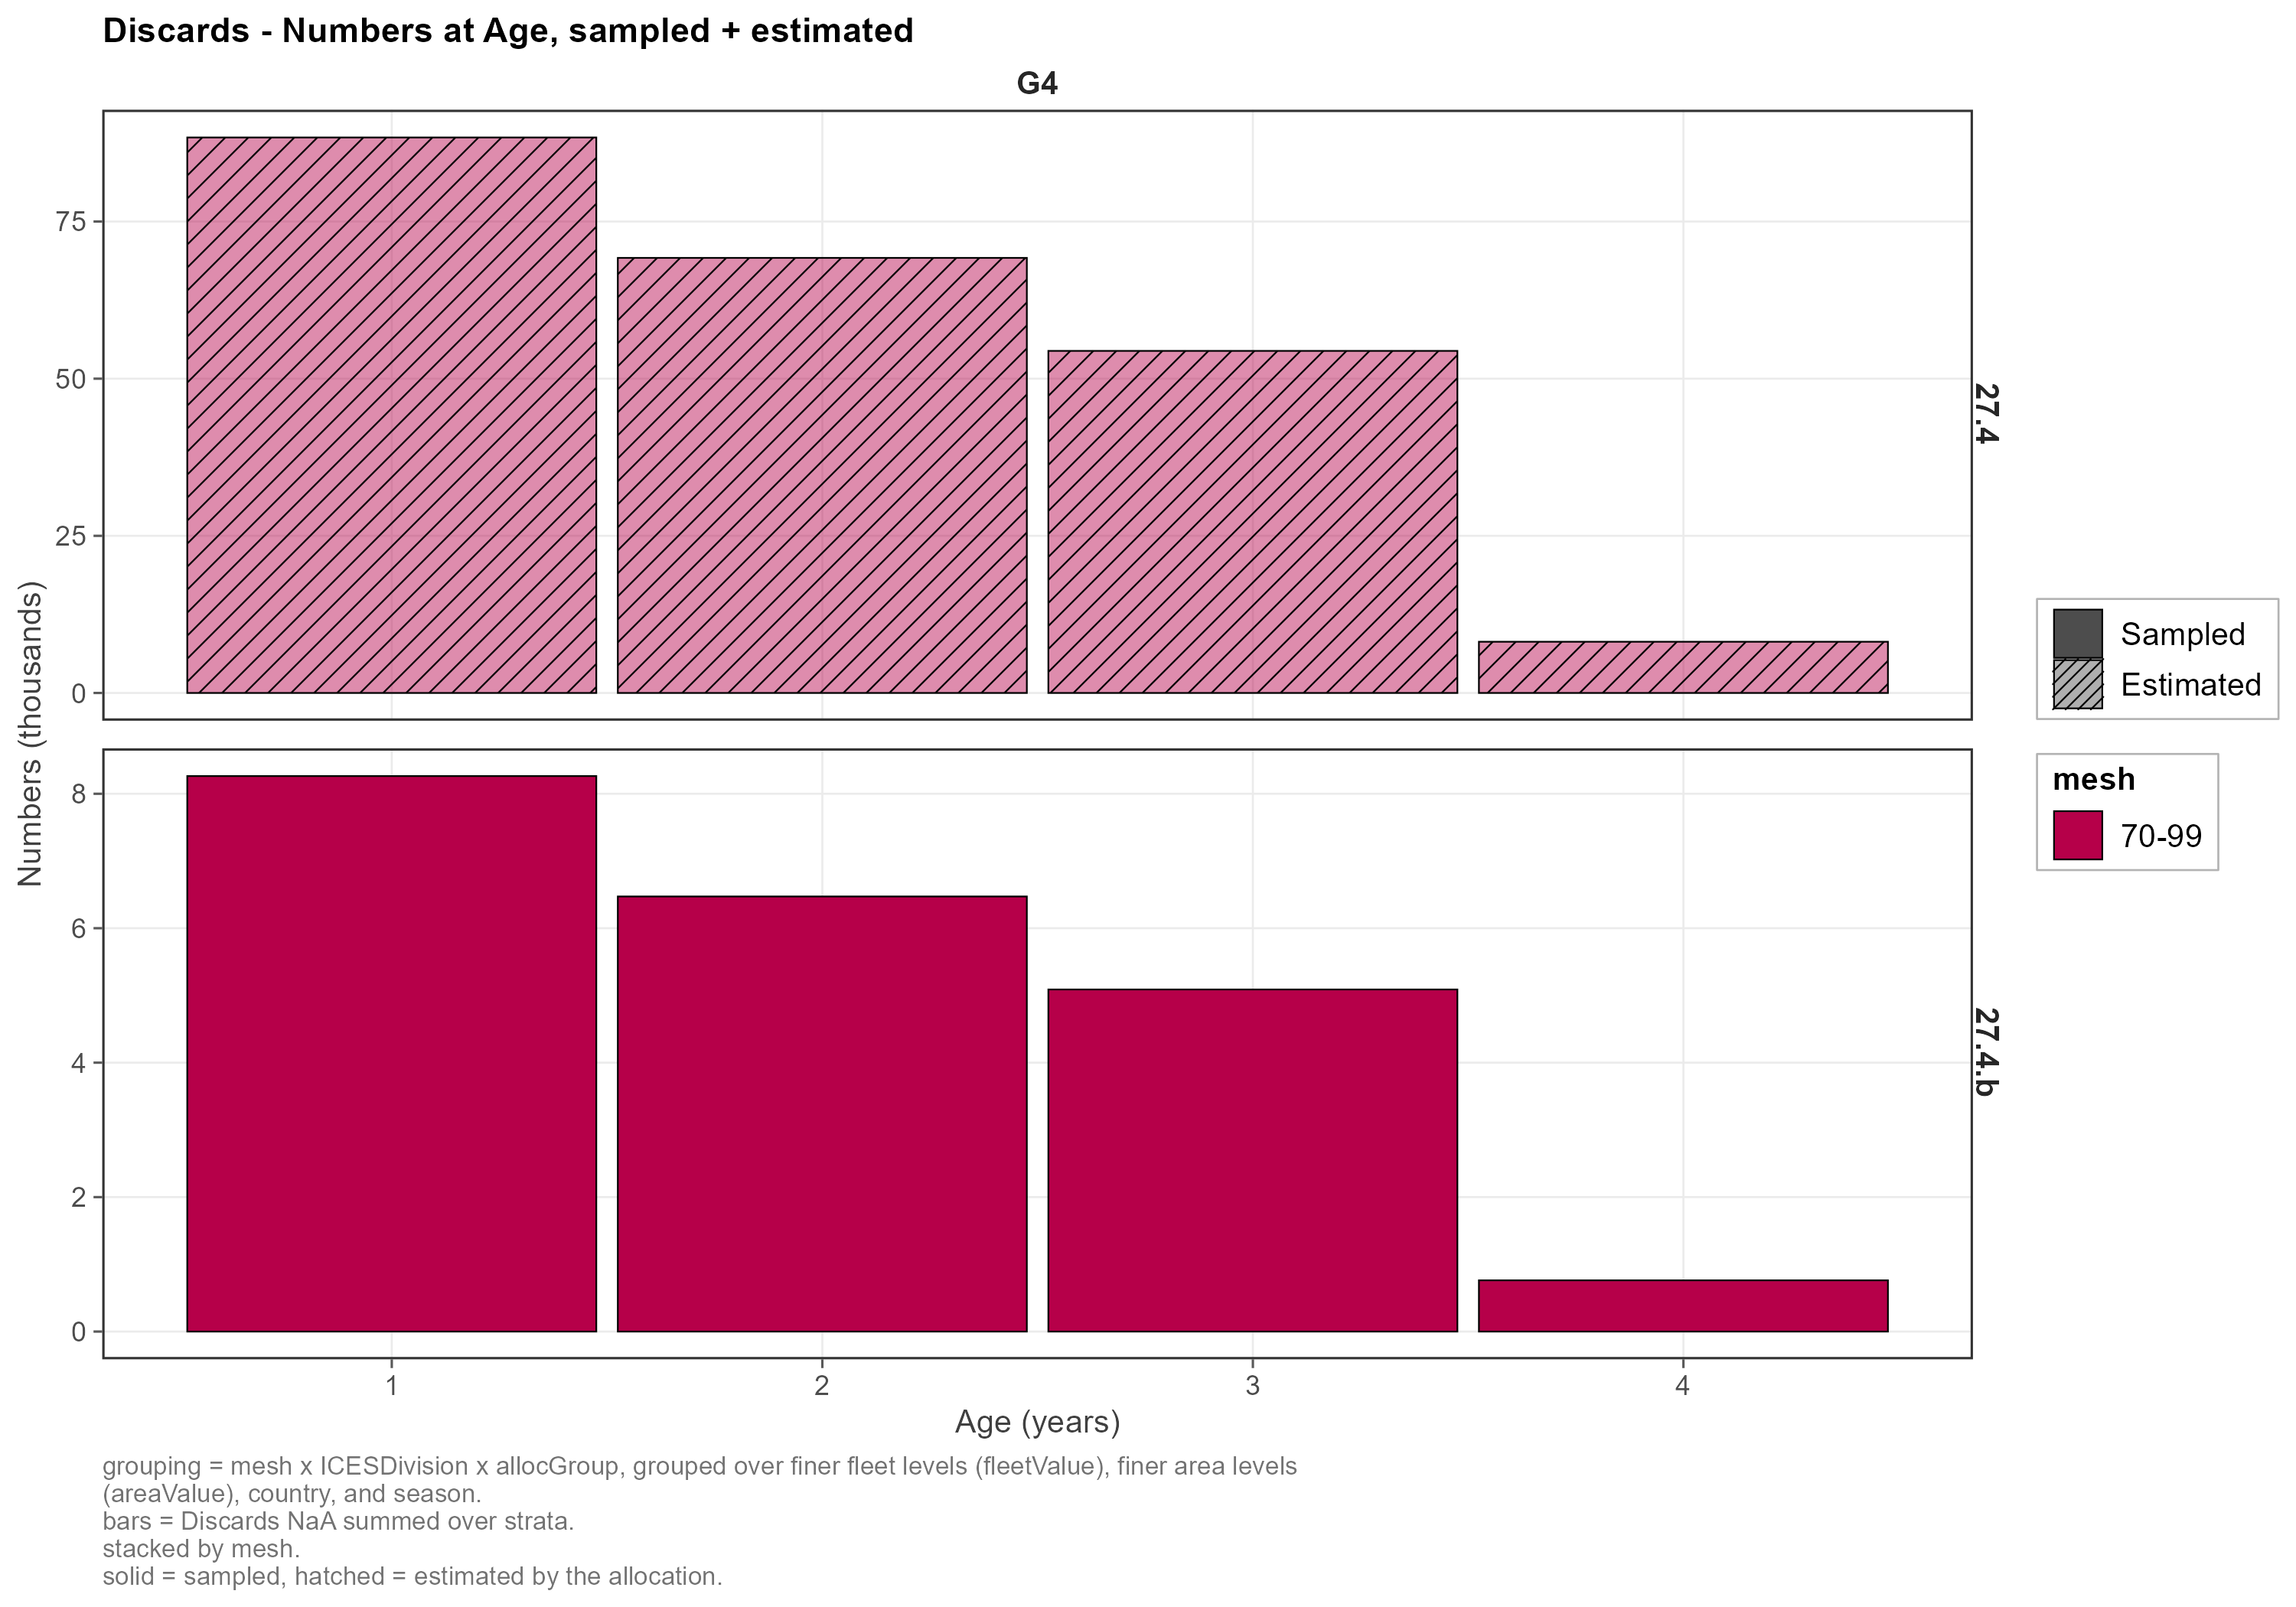
\includegraphics[width=1\linewidth,height=\textheight,keepaspectratio,alt={A grid of histograms of the numbers at age of the discards with the beam trawl group and the rest in columns and the ICES divisions in rows.}]{../../../output/figures/3_age_allocation/age_allocation_22.png}

}

\caption{\label{fig-nal-dis}Numbers at age of the discards, by ICES
division (rows) and allocation group (columns), filled by mesh: solid is
sampled, hatched is estimated. File \texttt{age\_allocation\_25.png}.}

\end{figure}%

The mean weight at age of the estimated distributions follows that of
the sampled ones (Figure~\ref{fig-mw}): the allocation keeps the
relation between age and weight of each group.

\begin{figure}[htbp]

\centering{

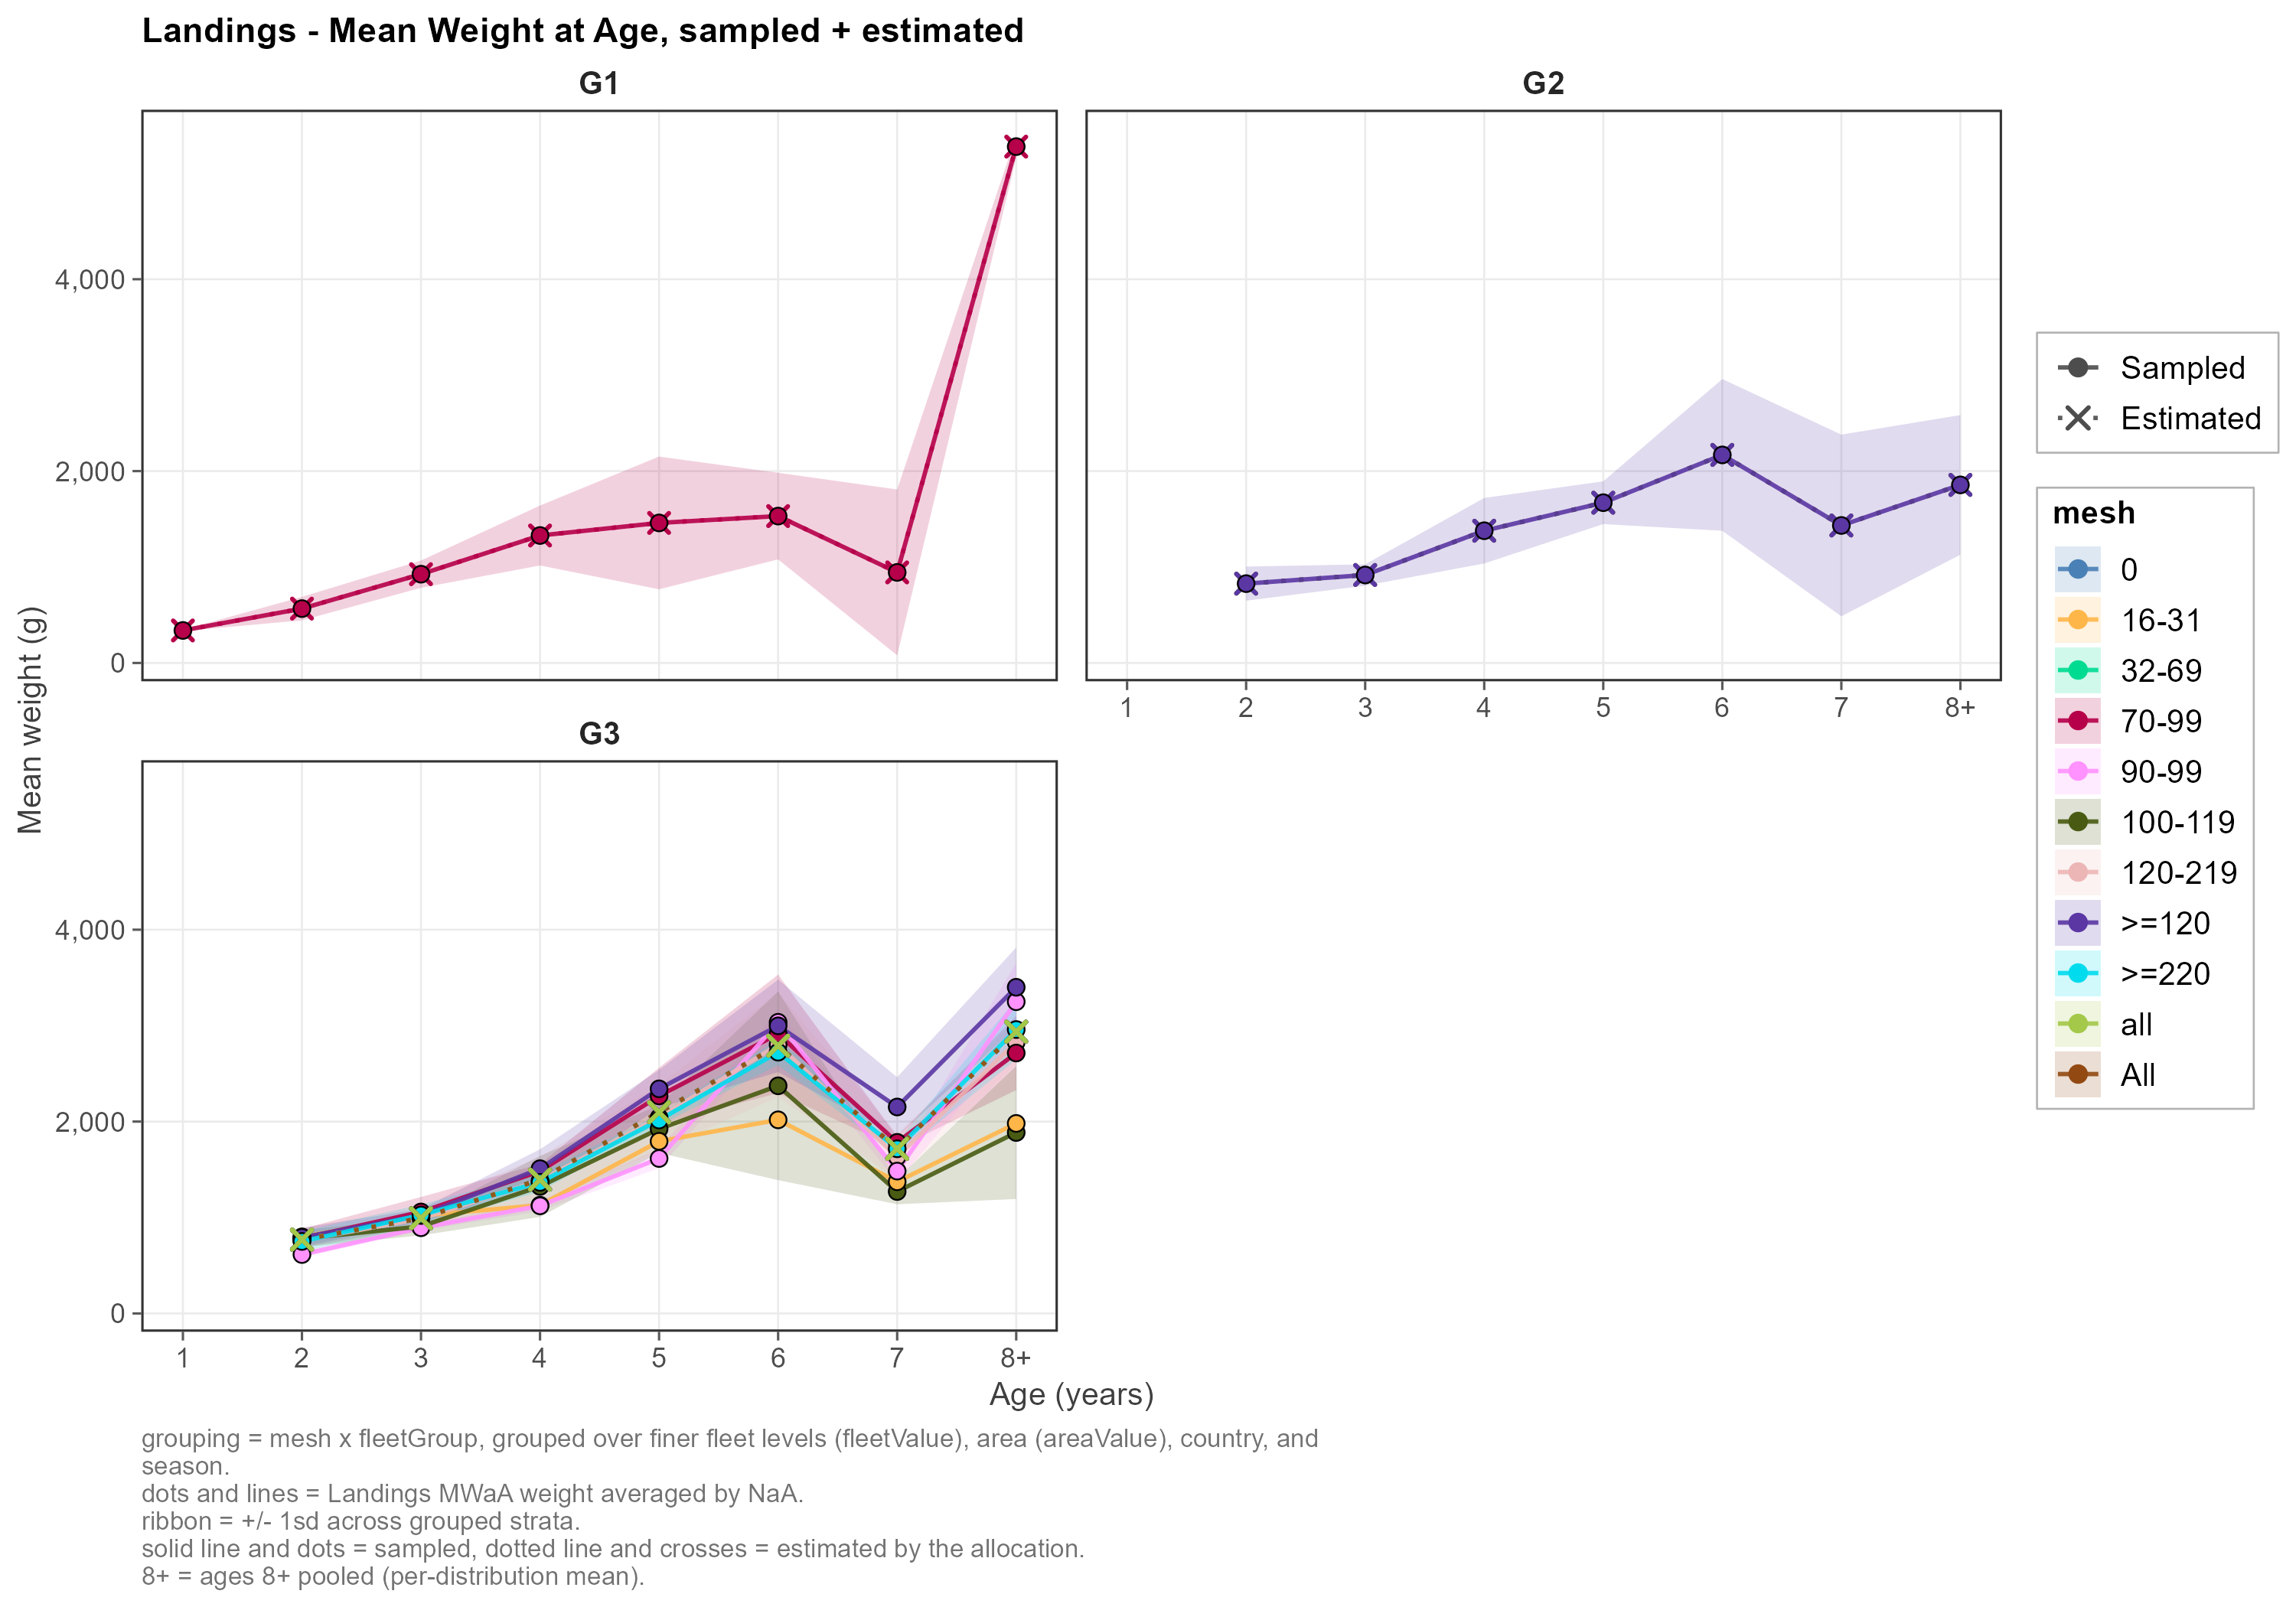
\includegraphics[width=1\linewidth,height=\textheight,keepaspectratio,alt={Four panels of mean weight in grams against age, sampled points and estimated crosses lying on the same curve.}]{../../../output/figures/3_age_allocation/age_allocation_24.png}

}

\caption{\label{fig-mw}Mean weight at age of the landings, by fleet
group and mesh (colour): dots and a solid line are sampled, crosses and
a dotted line are estimated by the allocation. File
\texttt{age\_allocation\_27.png}.}

\end{figure}%

\section{Aggregation and the two final
tables}\label{aggregation-and-the-two-final-tables}

\subsection{The aggregation functions}\label{the-aggregation-functions}

The two final tables are made by \texttt{catchCombined()} and
\texttt{distributionsCombined()} of \texttt{rcef}, in \texttt{output.R}.
Both add up over the strata and take the same \texttt{grouping}: the
year, the working group and the stock, the catch category, and what else
the stock assessment asks for. Here the catch is not split further, so
the grouping is the catch category. If the assessment asks for the catch
by season, area or fleet, these are added to the \texttt{grouping} of
both functions, since every distribution needs the catch it belongs to
in the CC.

\textbf{\texttt{catchCombined()}} adds up the working group's catch
(\texttt{originType\_catch\ =\ "WGEstimate"}, weights) of the raised
catch, in tonnes, by catch category, and writes the header of the file:
the year of the working group, the version and its description, whether
the year is the calendar year and, if it is not, the day the model year
starts. The sampling behind each total (\texttt{PSU}, \texttt{numPSUs},
\texttt{numTrips}) is taken from the columns of the catch with those
names and summed over the rows added up; a raised row, whose rate was
borrowed from a group, leaves its counts out. A raised row with no ratio
(no donor) adds up as nothing.

\textbf{\texttt{distributionsCombined()}} takes the distributions of the
allocation. It links each distribution to the catch it describes through
its domain: a sampled one through \texttt{domainBiology}, an estimated
one through the domain the allocation made up for the stratum (a name
that starts with \texttt{{[}alloc{]}\_}), so every stratum, raised or
not, sampled or estimated, finds its distribution. The numbers at age
are added up over all the strata of the category, in thousands of fish
(unit \texttt{NE3}), and the mean weight at age is the average of the
strata's mean weights, in g, weighted by their numbers at that age
(\texttt{weighting\ =\ "NumberAtAoL"}). The result has the long format
of the SCF: for each age class a \texttt{Number} row (value type
\texttt{Total}) and a \texttt{WeightLive} row (value type
\texttt{Mean}); a class with no fish is left out. The function warns
when it finds a catch weight with no distribution, or a distribution
with fish and no catch weight. The sampling of each class (\texttt{PSU},
\texttt{numPSUs}, \texttt{numTrips}, \texttt{numMeasurements}) is that
of the sampled distributions it is made of, each counted once; the
estimated ones were borrowed and have none.

\emph{(this code is no longer in the script)}

\emph{(this code is no longer in the script)}

The same numbers can be had with one column per age class
(\texttt{catchAtAoLAggregation()} and
\texttt{meanWoLatAoLAggregation()}, also in \texttt{output.R}) for a
look; they are not part of the SCF.

\subsection{Catch Combined}\label{catch-combined}

The CC has one row per catch category (Table~\ref{tbl-cc}): 1,669.5 t of
landings and 107.8 t of discards, 1,777.3 t in all. The row of the
landings below the minimum size (BMS) is 0.0 t. The fields of the SCF
that the catch is not split by (season, area, fleet) and the variance
are empty. The sampling behind the totals (\texttt{PSU},
\texttt{numPSUs}, \texttt{numTrips}) is the sum over the strata that
report it, and is empty for a catch category with none.

\begin{longtable}[]{@{}
  >{\raggedright\arraybackslash}p{(\linewidth - 6\tabcolsep) * \real{0.2317}}
  >{\raggedleft\arraybackslash}p{(\linewidth - 6\tabcolsep) * \real{0.2561}}
  >{\raggedleft\arraybackslash}p{(\linewidth - 6\tabcolsep) * \real{0.2561}}
  >{\raggedleft\arraybackslash}p{(\linewidth - 6\tabcolsep) * \real{0.2561}}@{}}

\caption{\label{tbl-cc}The Catch Combined (\texttt{output/SCF\_CC.csv}):
one column for each row of the file, named by its catch category, with
the fields that are filled; the others are empty.}

\tabularnewline

\toprule\noalign{}
\begin{minipage}[b]{\linewidth}\raggedright
Field
\end{minipage} & \begin{minipage}[b]{\linewidth}\raggedleft
BMS
\end{minipage} & \begin{minipage}[b]{\linewidth}\raggedleft
Dis
\end{minipage} & \begin{minipage}[b]{\linewidth}\raggedleft
Lan
\end{minipage} \\
\midrule\noalign{}
\endhead
\bottomrule\noalign{}
\endlastfoot
recordType & CC & CC & CC \\
version & 1 & 1 & 1 \\
versionDescription & RDBESstockCoord test & RDBESstockCoord test &
RDBESstockCoord test \\
calendarYear & Y & Y & Y \\
year & 2025 & 2025 & 2025 \\
workingGroup & WGNSSK & WGNSSK & WGNSSK \\
stock & tur.27.4 & tur.27.4 & tur.27.4 \\
variableType & WeightLive & WeightLive & WeightLive \\
variableUnit & t & t & t \\
total & 0.0 & 107.8 & 1,669.5 \\
numTrips & & & \\

\end{longtable}

\subsection{Distributions Combined}\label{distributions-combined}

The DC has 44 rows: 18 age classes for the landings and 4 for the
discards, each with a \texttt{Number} row and a \texttt{WeightLive} row
(Table~\ref{tbl-dc}). Figure~\ref{fig-dc} draws it: the numbers at age,
in thousands of fish, and the mean weight at age, in g, for the landings
and the discards.

\begin{longtable}[]{@{}
  >{\raggedright\arraybackslash}p{(\linewidth - 10\tabcolsep) * \real{0.1900}}
  >{\raggedleft\arraybackslash}p{(\linewidth - 10\tabcolsep) * \real{0.2400}}
  >{\raggedright\arraybackslash}p{(\linewidth - 10\tabcolsep) * \real{0.1800}}
  >{\raggedright\arraybackslash}p{(\linewidth - 10\tabcolsep) * \real{0.1400}}
  >{\raggedright\arraybackslash}p{(\linewidth - 10\tabcolsep) * \real{0.1300}}
  >{\raggedright\arraybackslash}p{(\linewidth - 10\tabcolsep) * \real{0.1200}}@{}}

\caption{\label{tbl-dc}The Distributions Combined
(\texttt{output/SCF\_DC.csv}): the first two age classes of each catch
category, a \texttt{Number} row (thousands of fish, \texttt{NE3}) and a
\texttt{WeightLive} row (mean weight, g) for each. All rows have the
distribution type \texttt{ageTotal}, in mm. The file has the rest of the
fields too: the header, and the sampling behind each row (\texttt{PSU},
\texttt{numPSUs}, \texttt{numTrips}, \texttt{numMeasurements}); the ones
the data does not fill are empty.}

\tabularnewline

\toprule\noalign{}
\begin{minipage}[b]{\linewidth}\raggedright
catchCategory
\end{minipage} & \begin{minipage}[b]{\linewidth}\raggedleft
distributionClass
\end{minipage} & \begin{minipage}[b]{\linewidth}\raggedright
variableType
\end{minipage} & \begin{minipage}[b]{\linewidth}\raggedright
variableUnit
\end{minipage} & \begin{minipage}[b]{\linewidth}\raggedright
valueType
\end{minipage} & \begin{minipage}[b]{\linewidth}\raggedright
value
\end{minipage} \\
\midrule\noalign{}
\endhead
\bottomrule\noalign{}
\endlastfoot
Dis & 1 & WeightLive & g & Mean & 321.520 \\
Dis & 1 & Number & NE3 & Total & 96.633 \\
Dis & 2 & WeightLive & g & Mean & 379.310 \\
Dis & 2 & Number & NE3 & Total & 75.687 \\
Lan & 1 & WeightLive & g & Mean & 339.010 \\
Lan & 1 & Number & NE3 & Total & 247.466 \\
Lan & 2 & WeightLive & g & Mean & 586.611 \\
Lan & 2 & Number & NE3 & Total & 466.057 \\

\end{longtable}

\begin{figure}[htbp]

\centering{

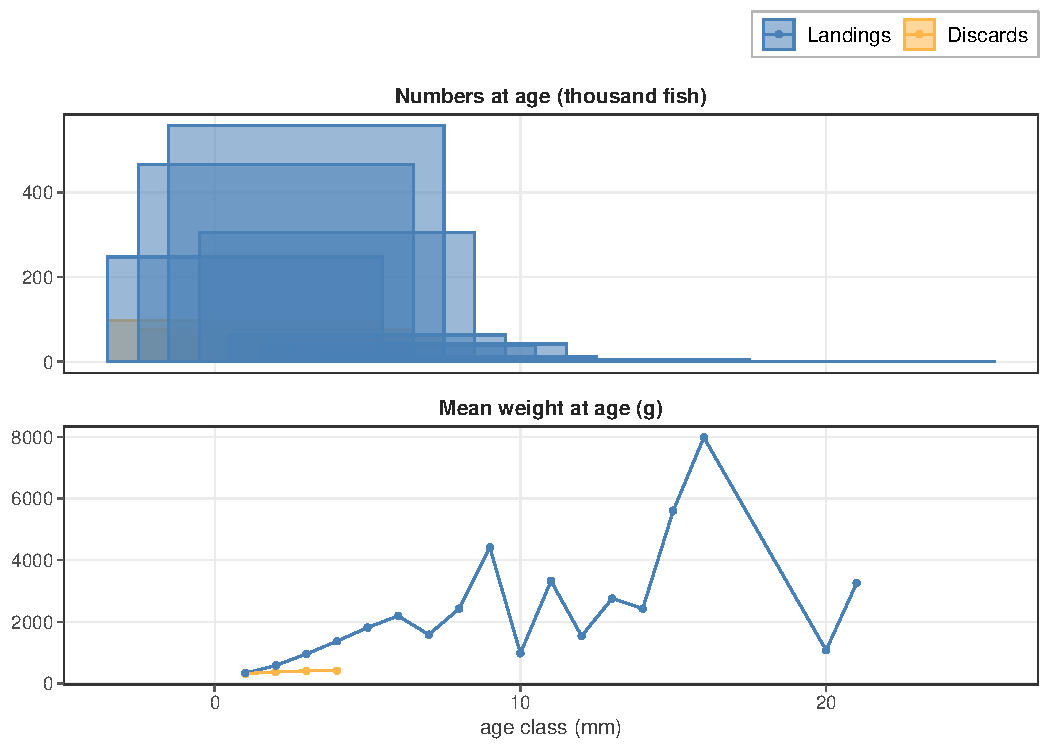
\includegraphics[width=1\linewidth,height=\textheight,keepaspectratio,alt={Two panels: bars of the numbers at age and lines of the mean weight at age, for the landings and the discards.}]{report_files/figure-pdf/fig-dc-1.pdf}

}

\caption{\label{fig-dc}The Distributions Combined: the numbers at age
(thousands of fish) and the mean weight at age (g) of the landings and
of the discards.}

\end{figure}%

\subsection{The check before
uploading}\label{the-check-before-uploading}

The SCF compares the catch of the CC with the sum of products of the DC
(the numbers times the mean weights, over the classes) and rejects a
total more than 20\% off. Here the two are at most 18.4\% apart
(Table~\ref{tbl-sop}).

\begin{longtable}[]{@{}
  >{\raggedright\arraybackslash}p{(\linewidth - 6\tabcolsep) * \real{0.1630}}
  >{\raggedleft\arraybackslash}p{(\linewidth - 6\tabcolsep) * \real{0.3261}}
  >{\raggedleft\arraybackslash}p{(\linewidth - 6\tabcolsep) * \real{0.2174}}
  >{\raggedleft\arraybackslash}p{(\linewidth - 6\tabcolsep) * \real{0.2935}}@{}}

\caption{\label{tbl-sop}The check of the SCF: the sum of products of the
DC against the catch of the CC.}

\tabularnewline

\toprule\noalign{}
\begin{minipage}[b]{\linewidth}\raggedright
Catch category
\end{minipage} & \begin{minipage}[b]{\linewidth}\raggedleft
Sum of products of the DC (t)
\end{minipage} & \begin{minipage}[b]{\linewidth}\raggedleft
Catch of the CC (t)
\end{minipage} & \begin{minipage}[b]{\linewidth}\raggedleft
Sum of products over catch
\end{minipage} \\
\midrule\noalign{}
\endhead
\bottomrule\noalign{}
\endlastfoot
Dis & 88.0 & 107.8 & 0.816 \\
Lan & 1,681.5 & 1,669.5 & 1.007 \\

\end{longtable}

The two files are \texttt{output/SCF\_CC.csv} (3 rows) and
\texttt{output/SCF\_DC.csv} (44 rows). Empty fields are left empty, and
the two are uploaded together.

\section{How this report is made}\label{how-this-report-is-made}

\texttt{report.R} renders \texttt{report.qmd} to html and pdf in
\texttt{report/}. The report reads the files the other scripts leave
(\texttt{data/}, \texttt{model/}, \texttt{output/}) and shows the
figures they saved in \texttt{output/figures/2\_discard\_raising/} and
\texttt{output/figures/3\_age\_allocation/}; it draws only the last
figure and computes only the small tables. The scripts are run in this
order: \texttt{data.R}, \texttt{model\_discard\_raising.R},
\texttt{model\_age\_allocation.R}, \texttt{output.R} and then
\texttt{report.R}. A figure or a table is as current as the script that
made its file.




\end{document}
